\documentclass[usenatbib]{mn2e} 
\usepackage{amsmath} 
\usepackage{amssymb} 
\usepackage{graphics}
\usepackage{graphicx}
\usepackage{epsfig}  
\def\be{\begin{equation}}
\def\ee{\end{equation}}
\def\ba{\begin{eqnarray}}
\def\ea{\end{eqnarray}}

% To highlight comments 
\usepackage{color}
\definecolor{red}{rgb}{1,0.0,0.0}
\newcommand{\red}{\color{red}}
\definecolor{blue}{rgb}{0.1,0.3,0.9}
\newcommand{\blue}{\color{blue}}

\usepackage[normalem]{ulem}
\definecolor{darkgreen}{rgb}{0.0,0.5,0.0}
\newcommand{\SRK}[1]{\textcolor{darkgreen}{\bf SRK: \textit{#1}}}
\newcommand{\SRKED}[1]{\textcolor{darkgreen}{\bf #1}}

\newcommand{\LCDM}{$\Lambda$CDM~}
\newcommand{\beq}{\begin{eqnarray}}  
\newcommand{\eeq}{\end{eqnarray}}  
\newcommand{\zz}{$z\sim 3$} 
\newcommand{\apj}{ApJ}  
\newcommand{\apjs}{ApJS}  
\newcommand{\apjl}{ApJL}  
\newcommand{\aj}{AJ}  
\newcommand{\mnras}{MNRAS}  
\newcommand{\mnrassub}{MNRAS accepted}  
\newcommand{\aap}{A\&A}  
\newcommand{\aaps}{A\&AS}  
\newcommand{\araa}{ARA\&A}  
\newcommand{\nat}{Nature}  
\newcommand{\physrep}{PhR}
\newcommand{\pasp}{PASP}    
\newcommand{\pasj}{PASJ}    
\newcommand{\avg}[1]{\langle{#1}\rangle}  
\newcommand{\ly}{{\ifmmode{{\rm Ly}\alpha}\else{Ly$\alpha$}\fi}}
\newcommand{\hMpc}{{\ifmmode{h^{-1}{\rm Mpc}}\else{$h^{-1}$Mpc }\fi}}  
\newcommand{\hGpc}{{\ifmmode{h^{-1}{\rm Gpc}}\else{$h^{-1}$Gpc }\fi}}  
\newcommand{\hmpc}{{\ifmmode{h^{-1}{\rm Mpc}}\else{$h^{-1}$Mpc }\fi}}  
\newcommand{\hkpc}{{\ifmmode{h^{-1}{\rm kpc}}\else{$h^{-1}$kpc }\fi}}  
\newcommand{\hMsun}{{\ifmmode{h^{-1}{\rm {M_{\odot}}}}\else{$h^{-1}{\rm{M_{\odot}}}$}\fi}}  
\newcommand{\hmsun}{{\ifmmode{h^{-1}{\rm {M_{\odot}}}}\else{$h^{-1}{\rm{M_{\odot}}}$}\fi}}  
\newcommand{\Msun}{{\ifmmode{{\rm {M_{\odot}}}}\else{${\rm{M_{\odot}}}$}\fi}}  
\newcommand{\msun}{{\ifmmode{{\rm {M_{\odot}}}}\else{${\rm{M_{\odot}}}$}\fi}}  
\newcommand{\lya}{{Lyman$\alpha$~}}
\newcommand{\clara}{{\texttt{CLARA}}~}
\newcommand{\rand}{{\ifmmode{{\mathcal{R}}}\else{${\mathcal{R}}$ }\fi}}  
\newcommand{\hs}{{\hspace{1mm}}}  

% definition to produce a "less than or similar to" symbol
\def\lsim{~\rlap{$<$}{\lower 1.0ex\hbox{$\sim$}}}

% definition to produce a "greater than or similar to" symbol
\def\gsim{~\rlap{$>$}{\lower 1.0ex\hbox{$\sim$}}}

\begin{document}

\title[Vweb \& Tweb]{Halo alignments with large scale tidal and velocity fields}
\author[S. Contreras et al.]{
\parbox[t]{\textwidth}{\raggedright 
  Sergio Contreras$^{1}$ 
  Jaime E. Forero-Romero$^{1}$ 
}
\vspace*{6pt}\\
$^{1}$Uni A
$^{2}$Uni B
}
\maketitle

\begin{abstract}

\end{abstract}
\begin{keywords}
methods: N-body simulations, galaxies: haloes, cosmology: theory, dark matter, large-scale structure of Universe
\end{keywords}


\section{Introduction}
\label{sec:introduction}

%-------

\section{Theoretical Antecedents}
\label{sec:theory}

... There is abundant literature on the issue of shape and angular momentum
aligmnent of dark matter haloe with respect to the cosmic we.

... This alignment is often measured from the distribution of the
$\cos\theta$ where $\theta$ is the angle between the two axes of
interest.

... Table 1 summarizes recent results found in the literature for
shape and angular momentum alignment.


\citep{Libeskind2013} %various alignments
\citep{Codis2012}
\citep{Faltenbacher2009} %galaxy alignments with mocks
\citep{Paz2008} %angular momentum alignments
\citep{Platen2008} %alignment in voids
\citep{Lee2007}%Obs. spin alignment



\begin{itemize}
\item
\citep{AragonCalvo2007} %Spin alignment
The method is the Multi-scale Morphology Filter which is based on the
Hessian matrix of the density field, where the density field is
computed from the particle distribution using a Delaunay tesselation
field estimatior (DTFE), which is self-adaptive. This allows them to
identify clusters, filaments and walls.


The simulation has $512^3$ particles in a cubic box of $150$\hMpc. The
mass per particle is $2\times 10^{9}$\hMsun. 
Halo identitification is done with the HOP algorithm. They keep halos with more
than $50$ partices and less than $5000$, defining a mass range of
$1-100\times 10^{11}$\hMsun.

The principal
axes of each halo are computed from the non-normalized inertia
tensor. The inertian tensor and the angular momentum are computed with
respect to the center of mass of the halo.


They compute two angles, one with respect to the direction
defining the filaments and the other the walls. Their results make a
distinction between halos of more massive and less massive than
$10^{12}$\hMsun.

The halo spins tend to lie on the plane of the wall. This is stronger
for massive halos.The effect for filaments is weaker: low mass halos
tend to lieparallel to their host filament, while high mass halos tend
to be perpendicular.  

Theres is a very strong effect for the principal axes of halos in
filaments to be strongly correlated with the direction of the
filaments. The minor axis tend to be perpendicular to the
filament. This effect is stronger for larger halos.

The effect in walls is less strong ,but still the minor axis tend to
lie perpendicular to the wall, while the other axis then to lie over
the wall. The effect is stronger for massive halos.

They find that spins and shapes of dark matter halos are significantly
correlated with each other and with the orientation of their host
structures. 



\item 
\citep{Hahn2007}% various alignments with the Tweb
The method is the Tweb. They use three simulations each of $512^3$
particles, with sizes $L_1=45$\hMpc, $L_2=90$\hMpc and
$L_3=180$\hMpc, this corresponds to particle masses of $4.7, 38.0,
300\times 10^7$\hMsun. The normalization is $\sigma_8=0.9$. Halo
identification was done with a FOF algorithm with 0.2 times the
interparticle distance. They consider halos of at least 300
particles. 

The web is obtained for a grid of $1024^3$ cells, the density field is
obtained with a CIC interpolation and smoothed using a Gaussian
Kernel. In the rest of the paper all the results correspond to a
smoothing scale of $R_{s}=2.1$\hMpc.


They Report on the angle between the halo
angular momentum vector and the eigenvector corresponding to
perpendicular directions to the sheets and the direction of the
filaments. This is divided in two halo populations: $5\times 10^{10} -
1.0\times 10^{12}$ and $>10^{12}$. There is a weak antialignment in
the case of the filaments and a stronger anti-alignment in the case of
the sheets. For the sheets the effect is stronger for the massive
bin. In the filaments the alignment is weak regardless of the
mass. They do not report any other significan statistic, but recognize
that they suffer from small-number statistics in voids).


They do not see any strong dependance of the environment in the
shape. They do not measure the shape alinment.

\citep{Lee2002}%Obs. spin alignment
Observational measurement for the alignment of galaxy spin axes with
the local tidal shear field. For the measurement of shear, we have used
the Point Source Catalog Redshift (PSCz) survey (a complete redshift survey
from the IRAS Point Source Catalog) data. This was done down to a
radial comoving distance of $\sim 150$\hMpc.
\item
\citep{Hatton2001} %angular momentum alignment
DM matter only simulation. $256^3$ particles, $100$\hMpc, particle
mass. Look for mutual alignment of angular momentum vectors, and
alignment with structure. halos on any escale by close pair
statistics. They don't find any evidence for a statistically significant mutual
alignment of haloes on any scale,
\end{itemize}
\section{N-body simulation and halo finding}


... In this paper we use groups found with a FOF halo finder.

\section{The cosmic web algorithms}
\label{sec:algorithms}

\subsection{The Tidal Web}



\subsection{The Velocity Web}

\subsection{Numerical considerations}

... In this paper we compute the cosmic web on grids of two different
resolutions $256^3$ and $512^3$.

\section{Results}

\subsection{Interweb Alignment}
... We compute the pair-wise allignment between the eigenvectors in
the two web finders. 

... We also compute the alignment between the eigenvectors in cells
occupied by dark matter halos. This will be a key element in the
interpretation of the results for halo-based allignments in the next
sections: shape, angular momentum and peculiar velocities.

... 

\begin{figure*}
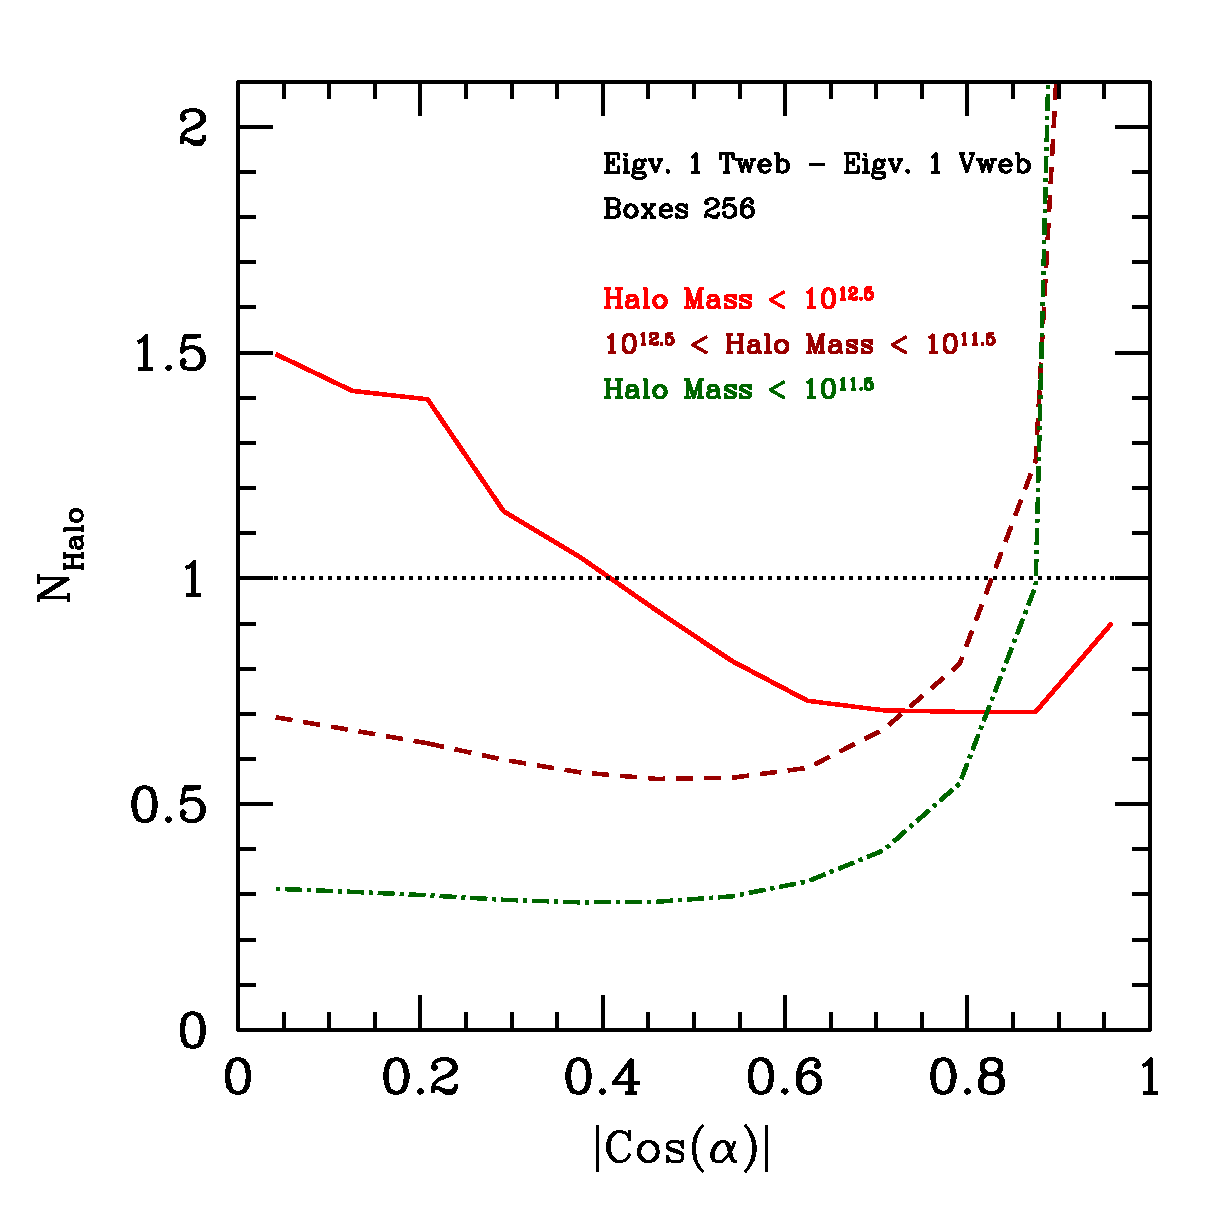
\includegraphics[width=0.30\textwidth]{../plot2/256/256_T1V1.ps}
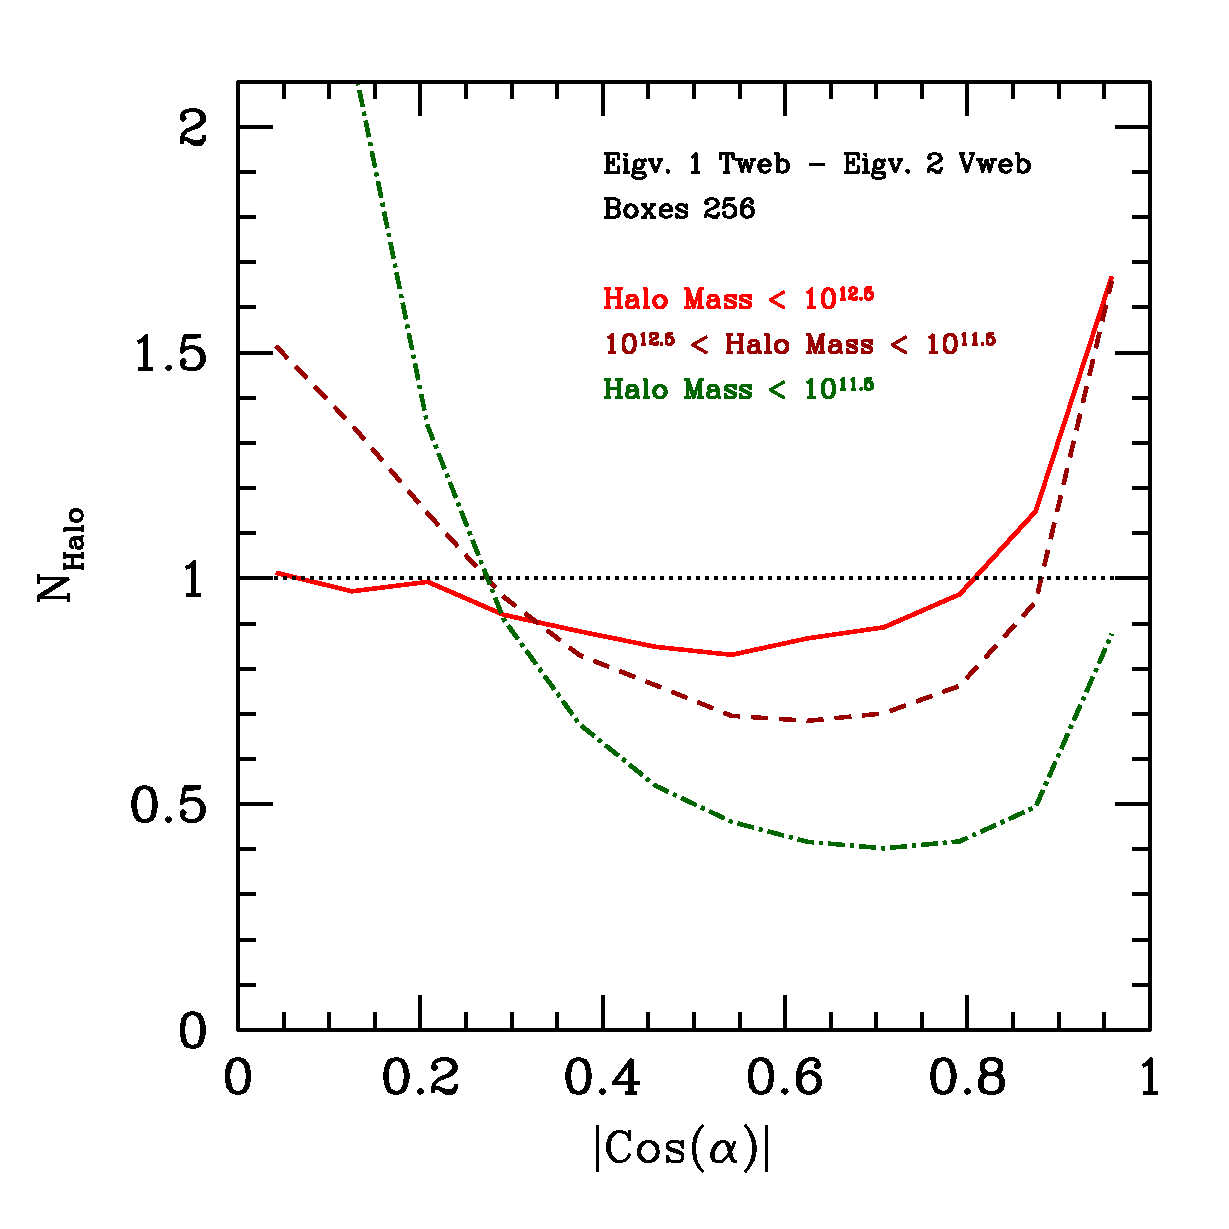
\includegraphics[width=0.30\textwidth]{../plot2/256/256_T1V2.ps}
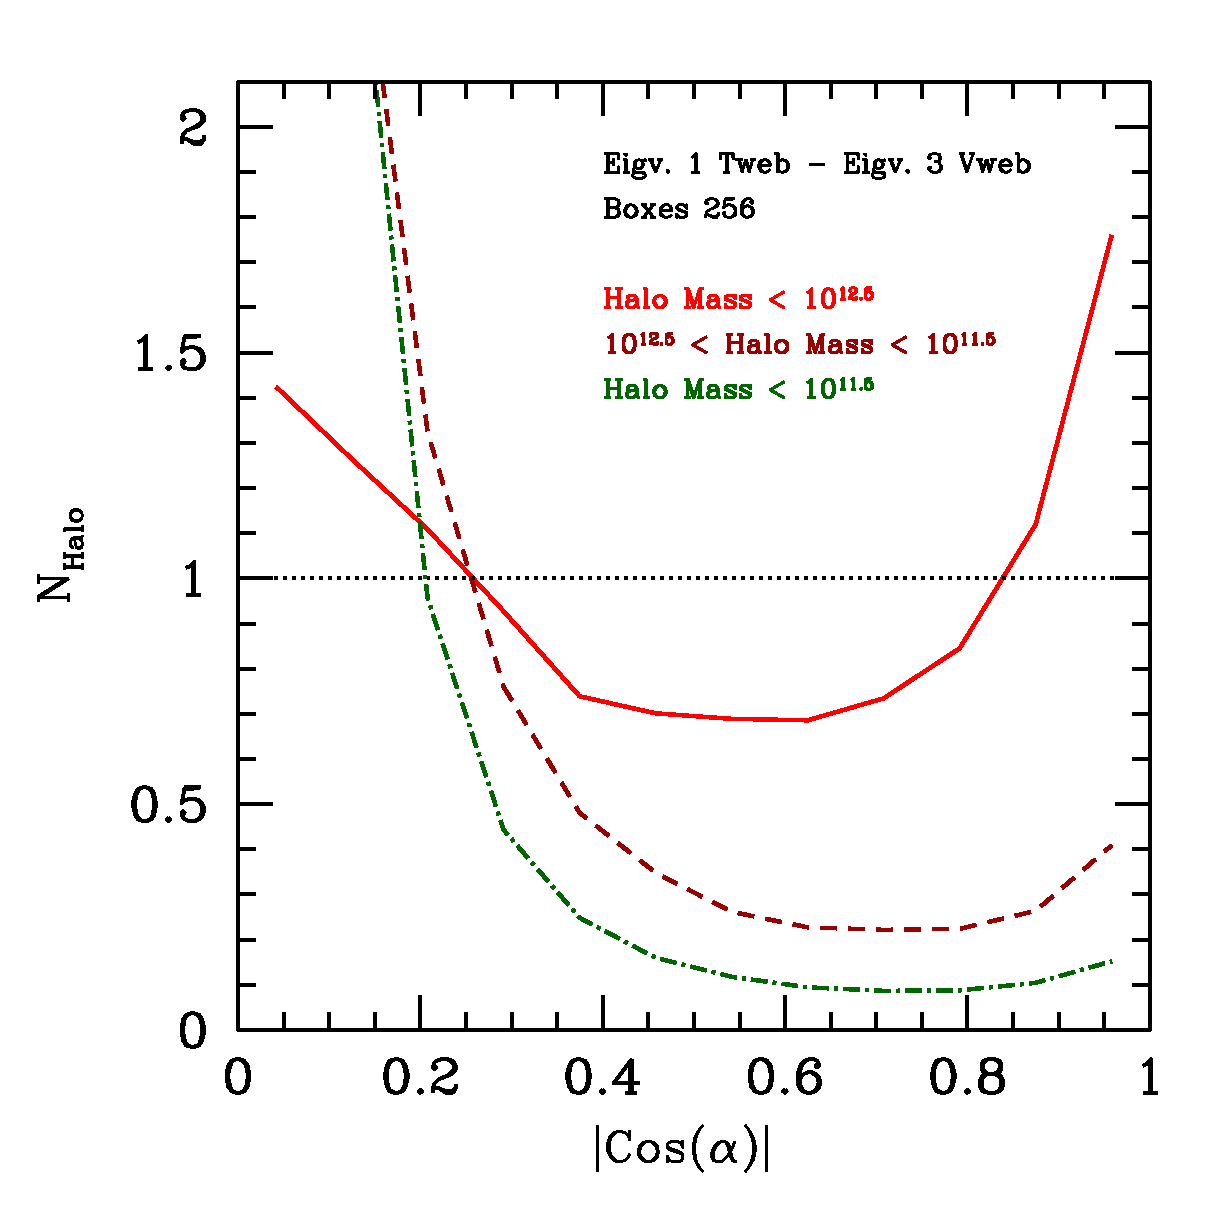
\includegraphics[width=0.30\textwidth]{../plot2/256/256_T1V3.ps}
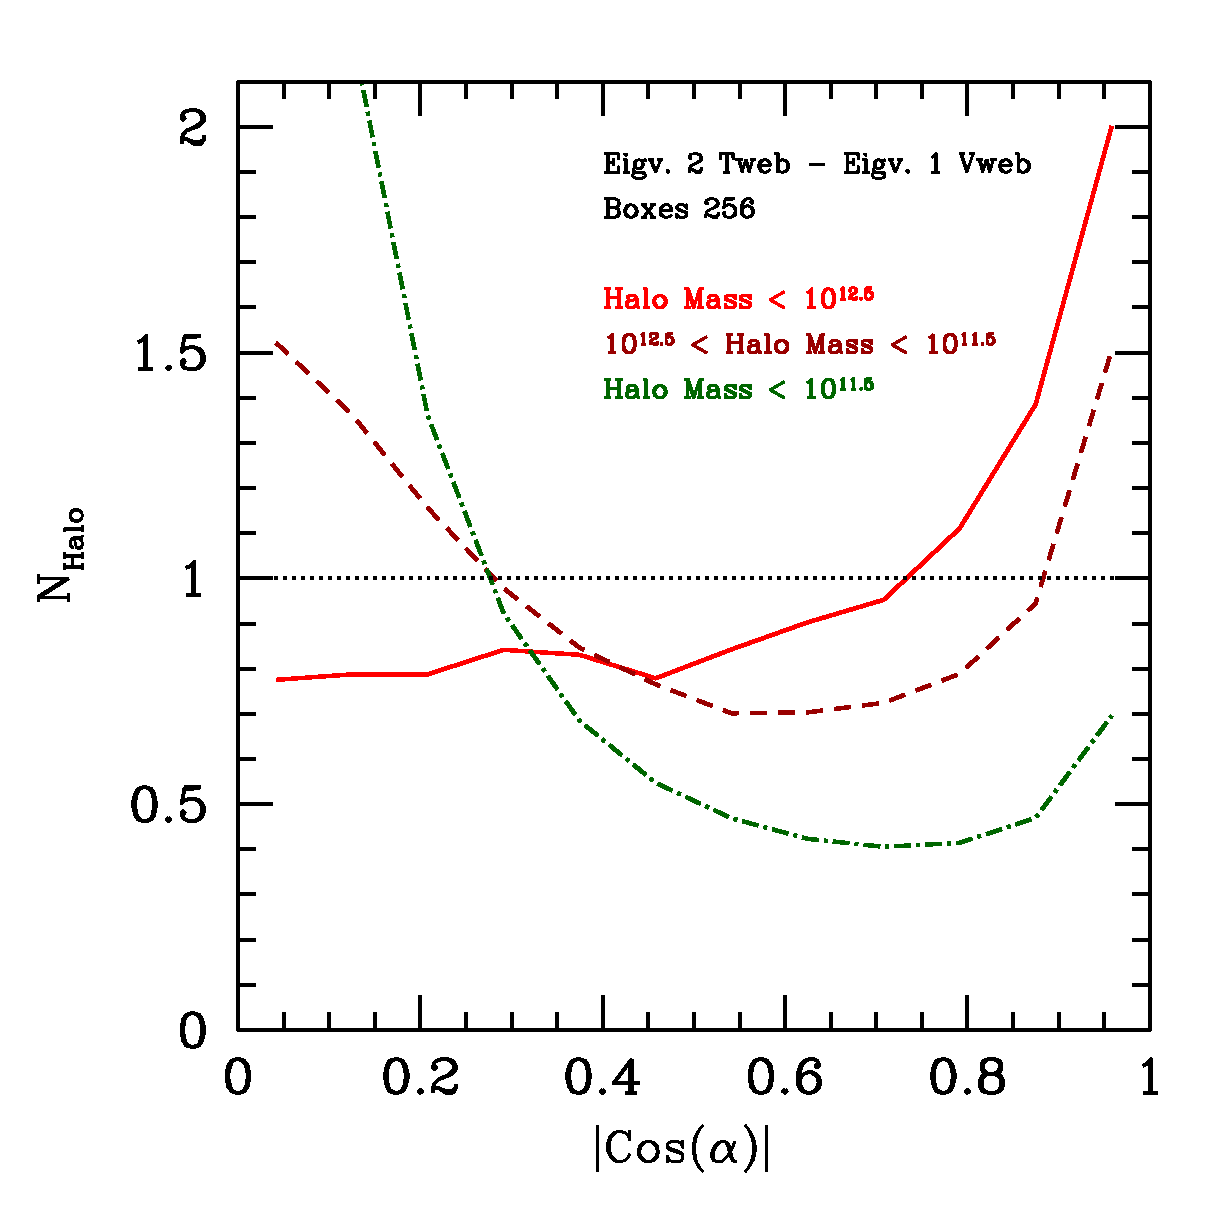
\includegraphics[width=0.30\textwidth]{../plot2/256/256_T2V1.ps}
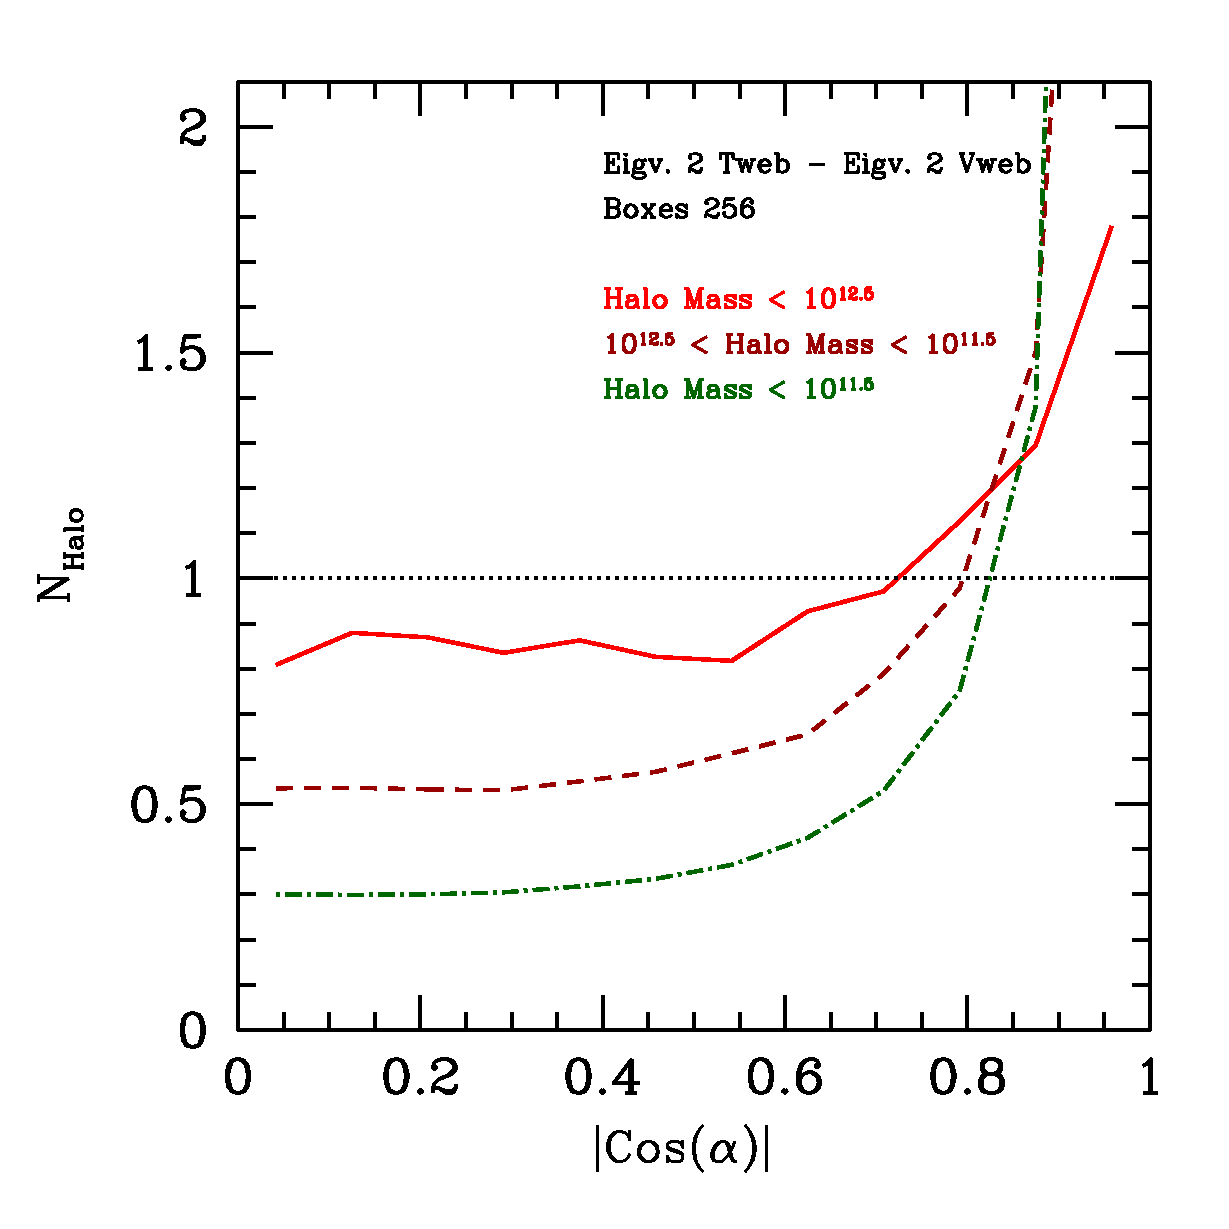
\includegraphics[width=0.30\textwidth]{../plot2/256/256_T2V2.ps}
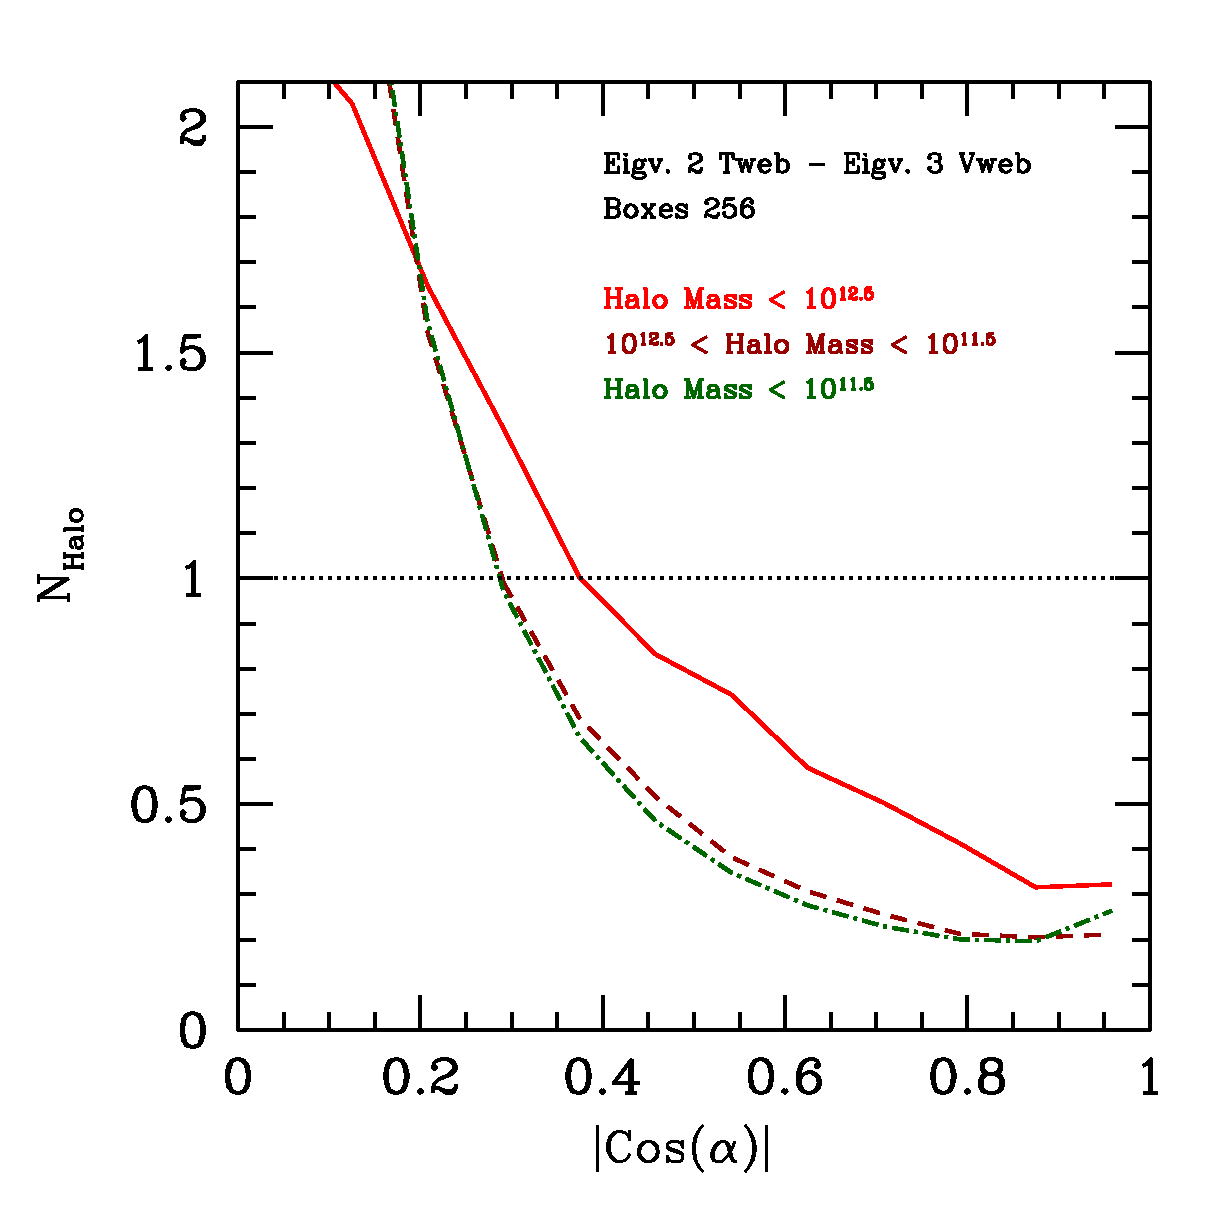
\includegraphics[width=0.30\textwidth]{../plot2/256/256_T2V3.ps}
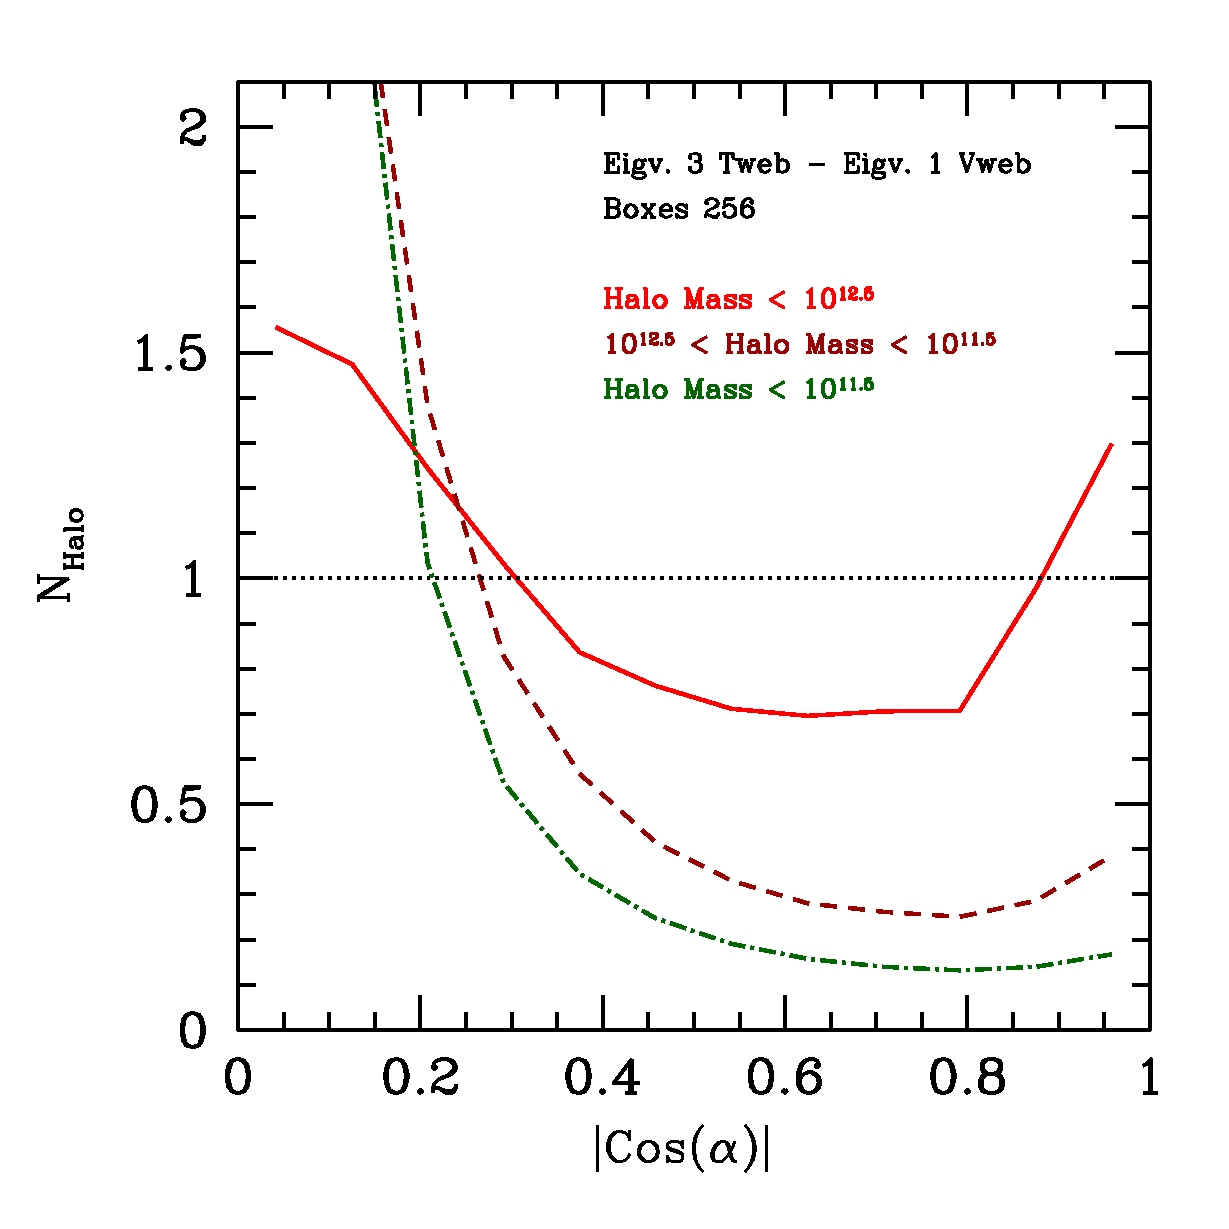
\includegraphics[width=0.30\textwidth]{../plot2/256/256_T3V1.ps}
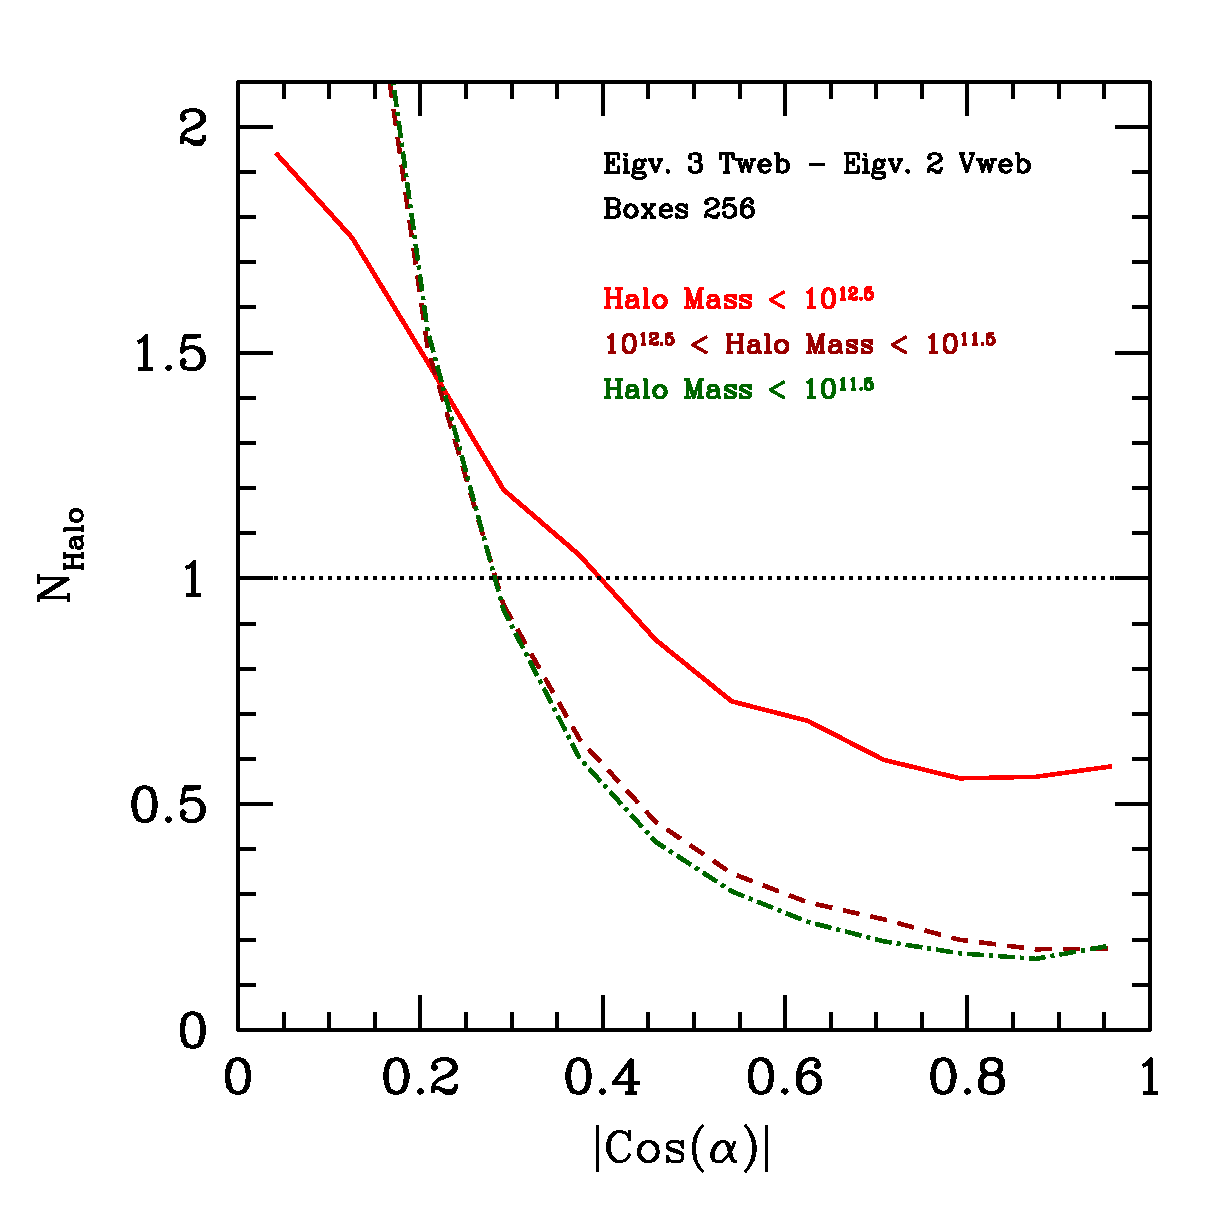
\includegraphics[width=0.30\textwidth]{../plot2/256/256_T3V2.ps}
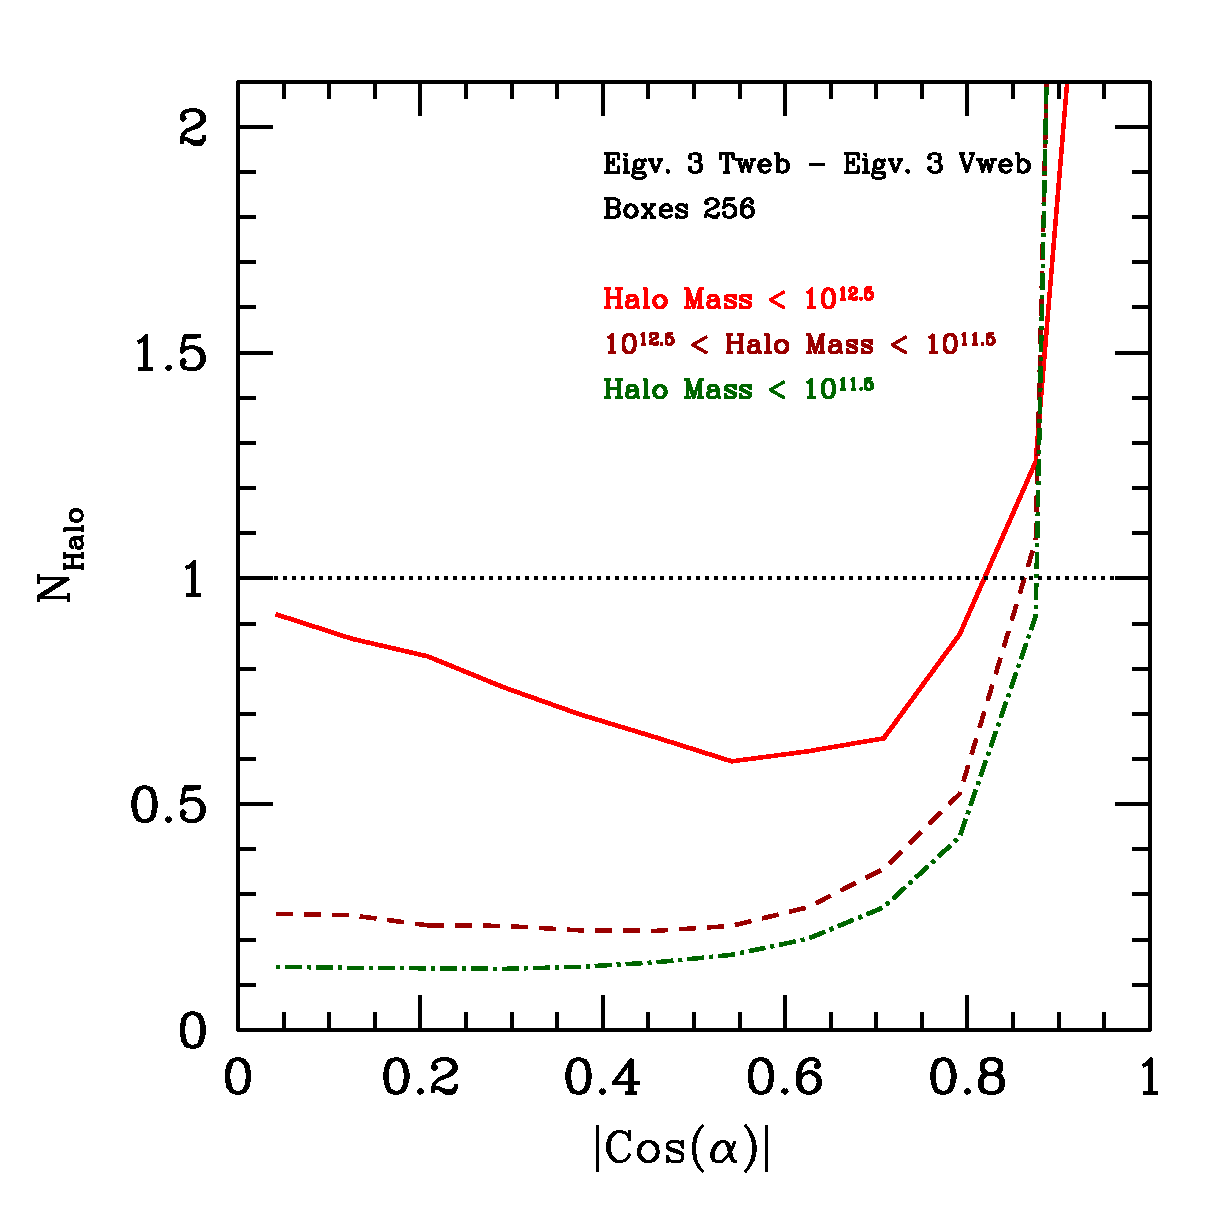
\includegraphics[width=0.30\textwidth]{../plot2/256/256_T3V3.ps}
\caption{Interweb alignment for $256^3$ grid resolution.}
\end{figure*}

\begin{figure*}
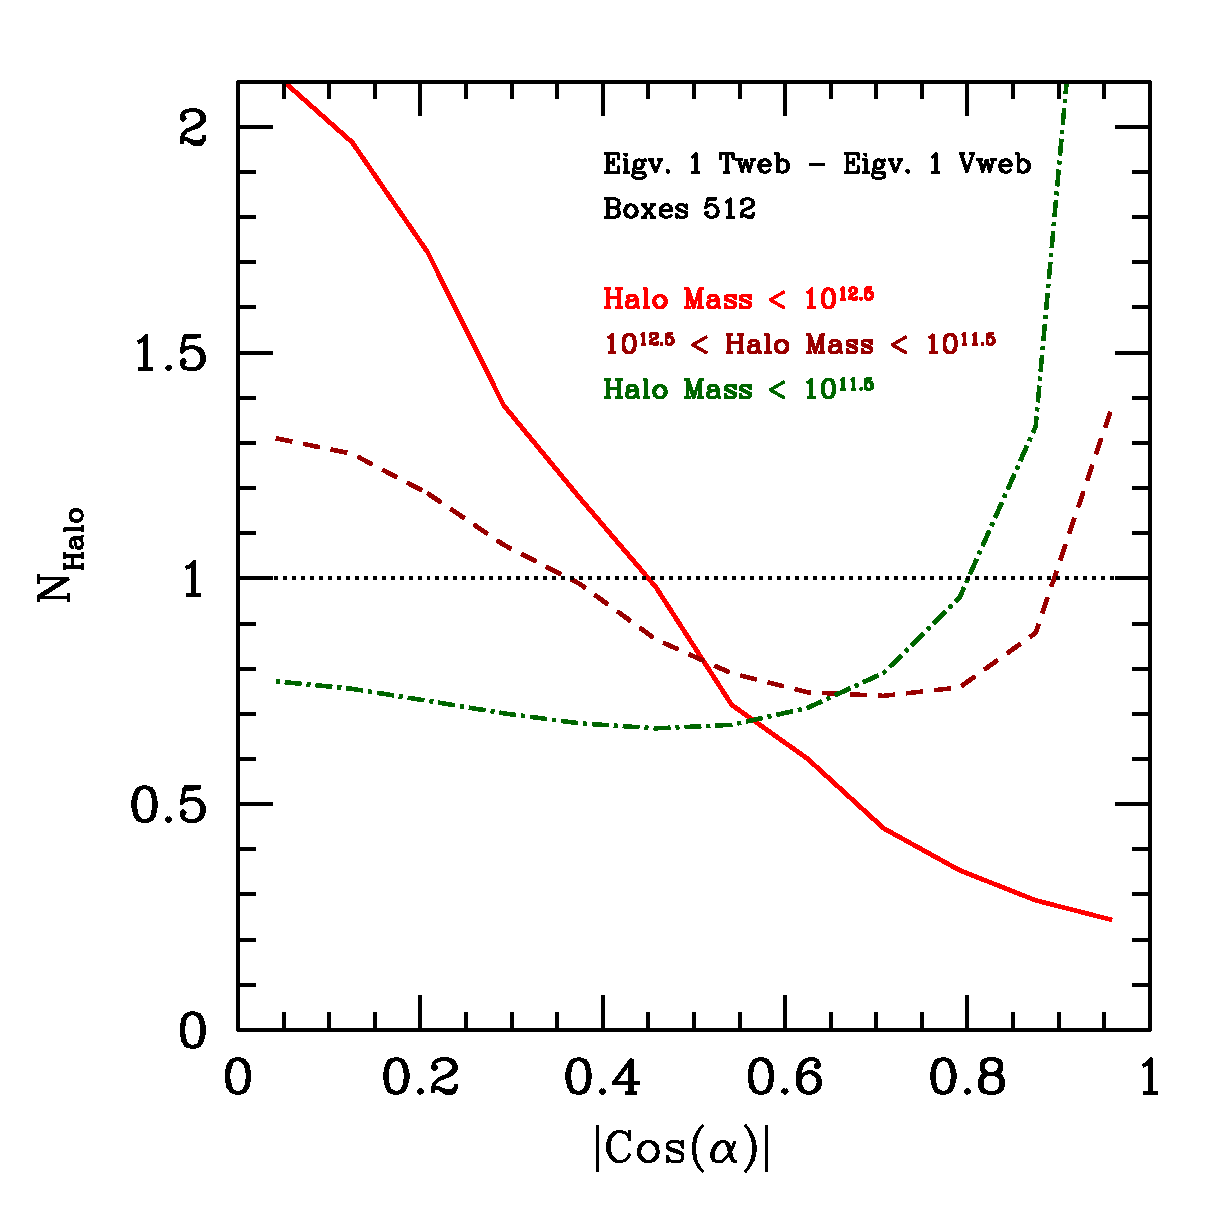
\includegraphics[width=0.30\textwidth]{../plot2/512/512_T1V1.ps}
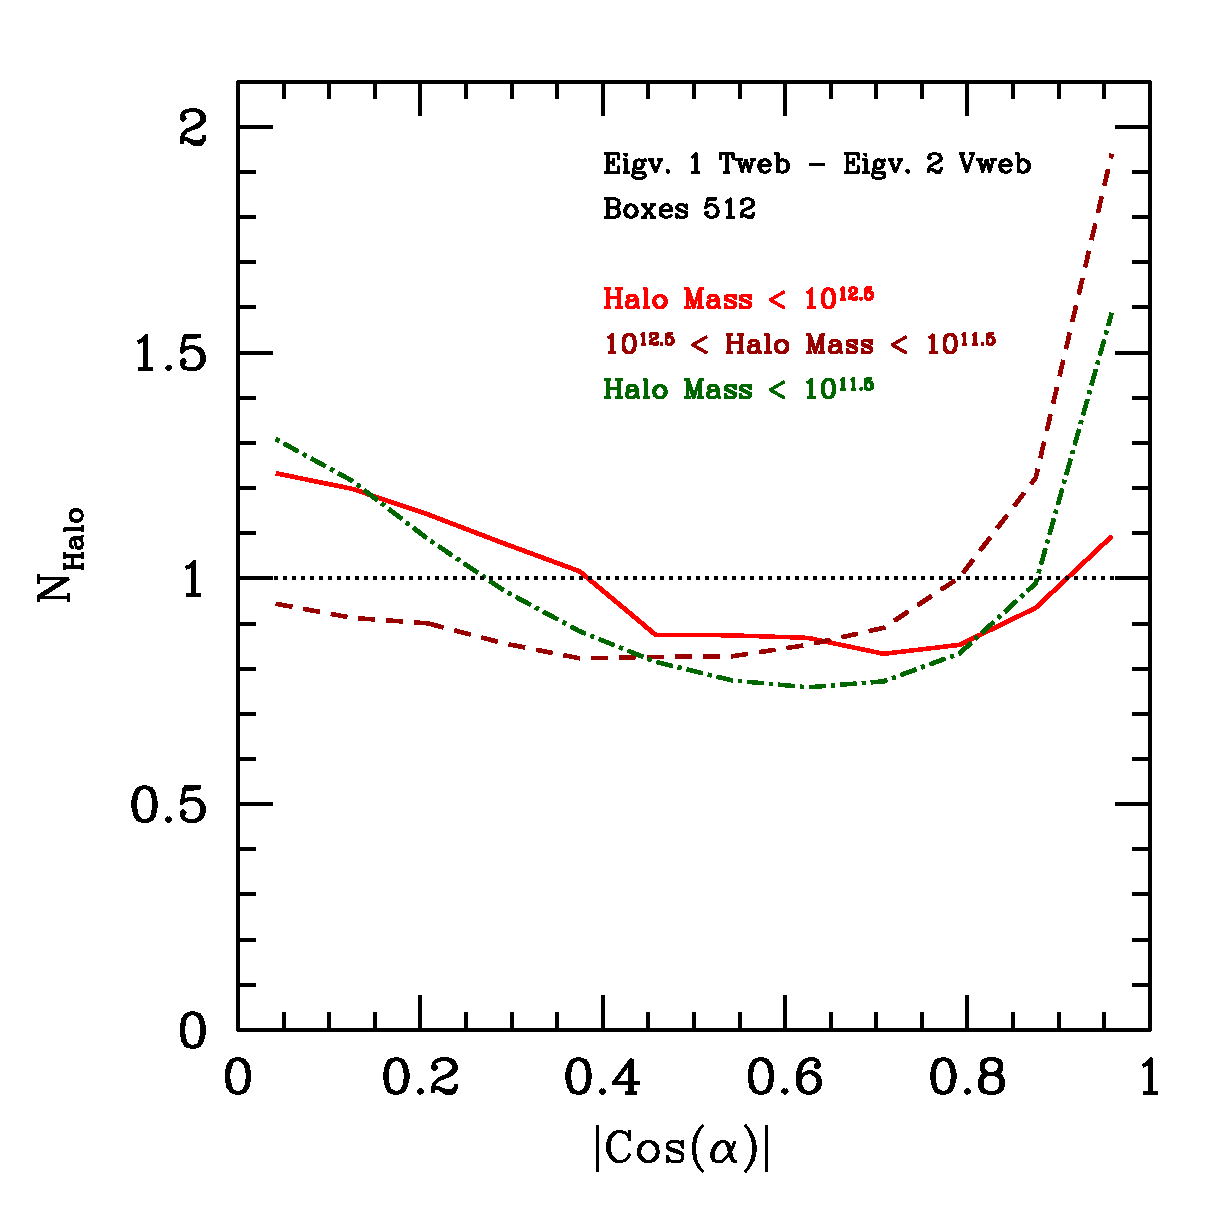
\includegraphics[width=0.30\textwidth]{../plot2/512/512_T1V2.ps}
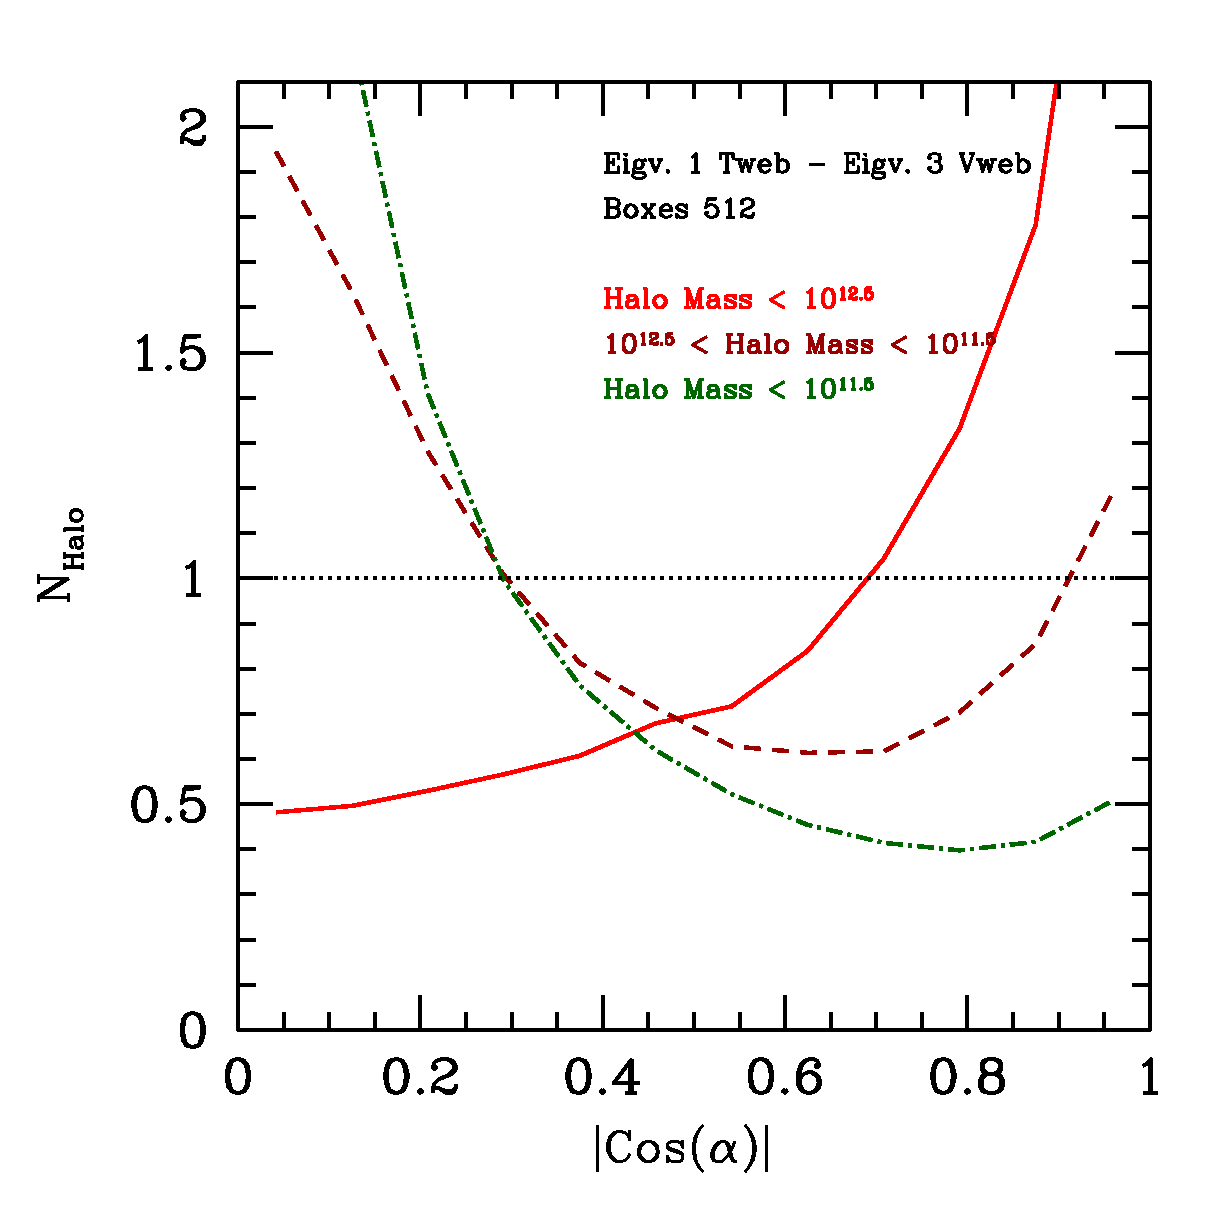
\includegraphics[width=0.30\textwidth]{../plot2/512/512_T1V3.ps}
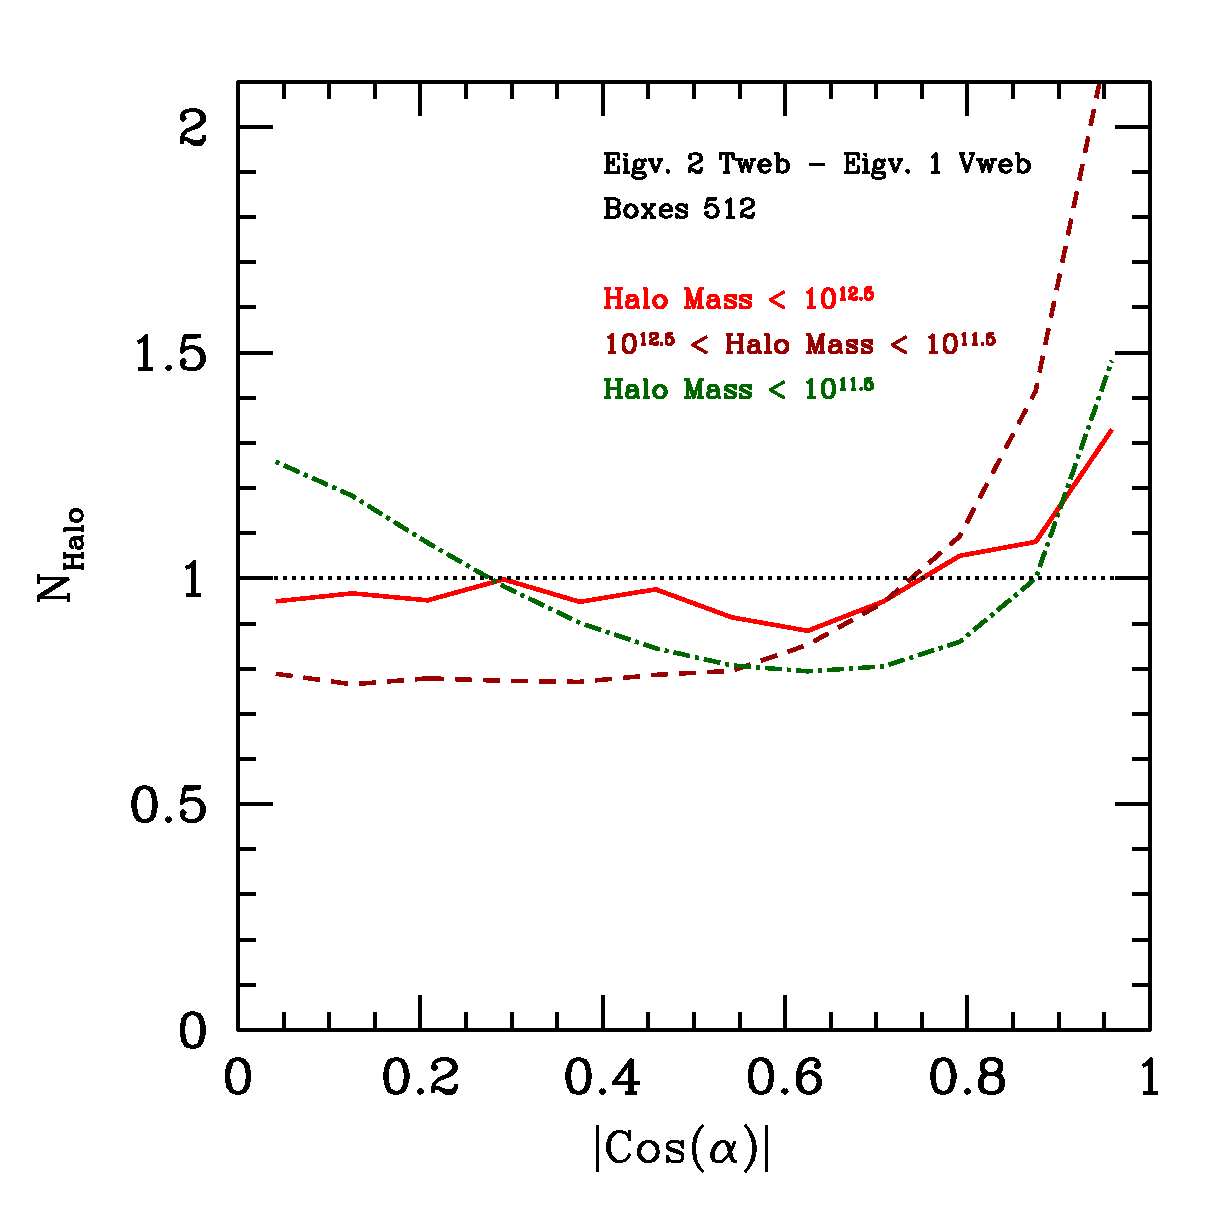
\includegraphics[width=0.30\textwidth]{../plot2/512/512_T2V1.ps}
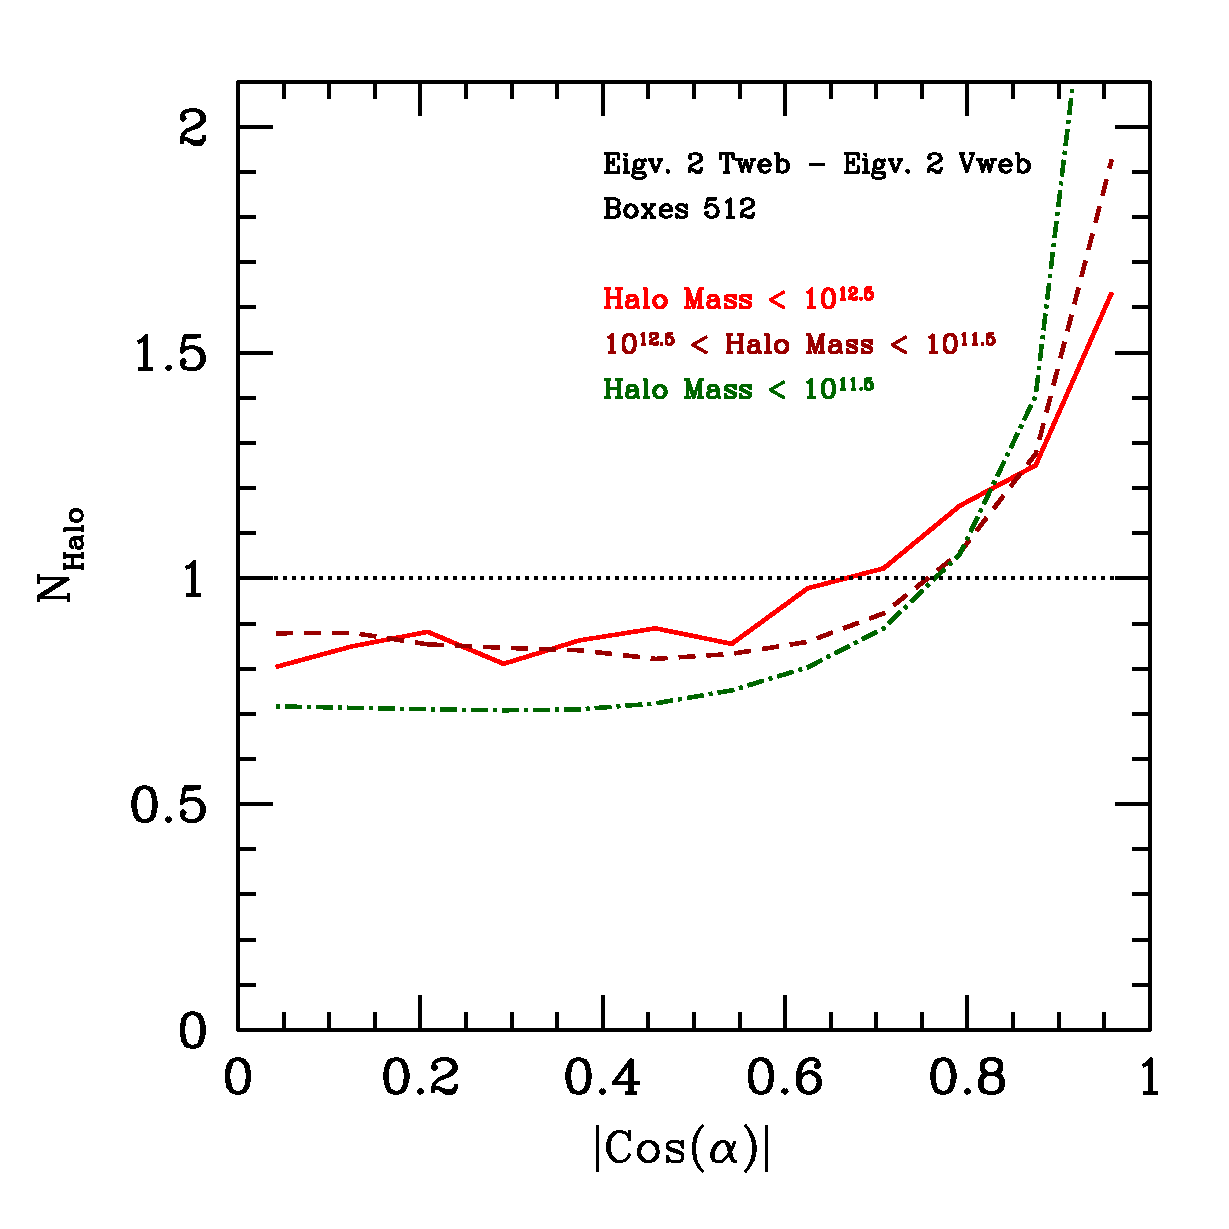
\includegraphics[width=0.30\textwidth]{../plot2/512/512_T2V2.ps}
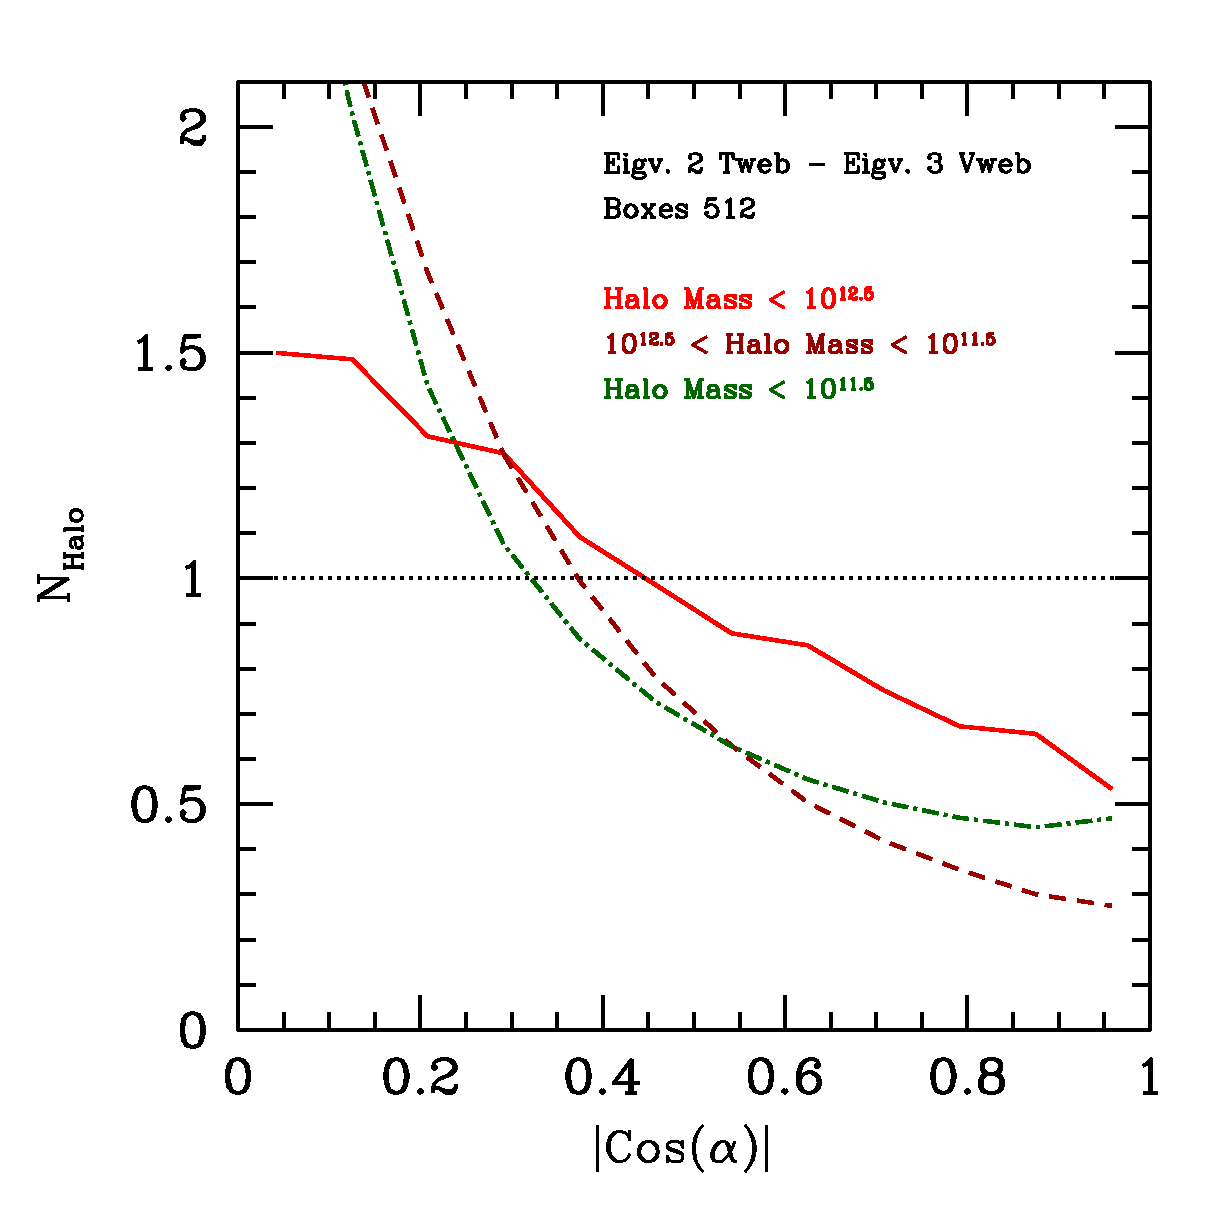
\includegraphics[width=0.30\textwidth]{../plot2/512/512_T2V3.ps}
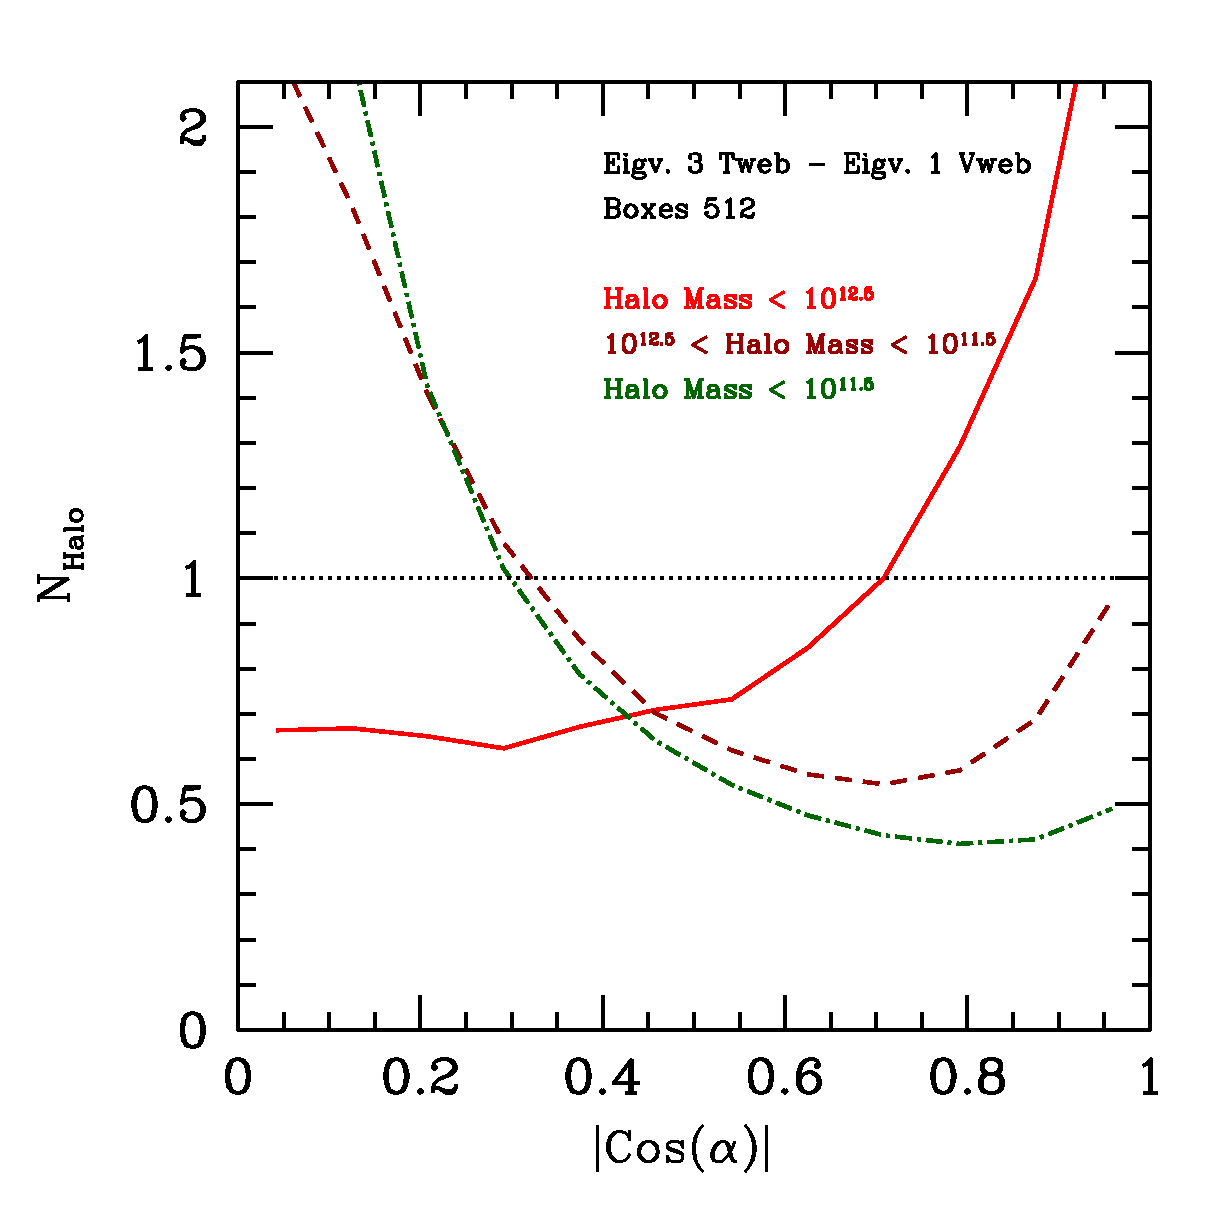
\includegraphics[width=0.30\textwidth]{../plot2/512/512_T3V1.ps}
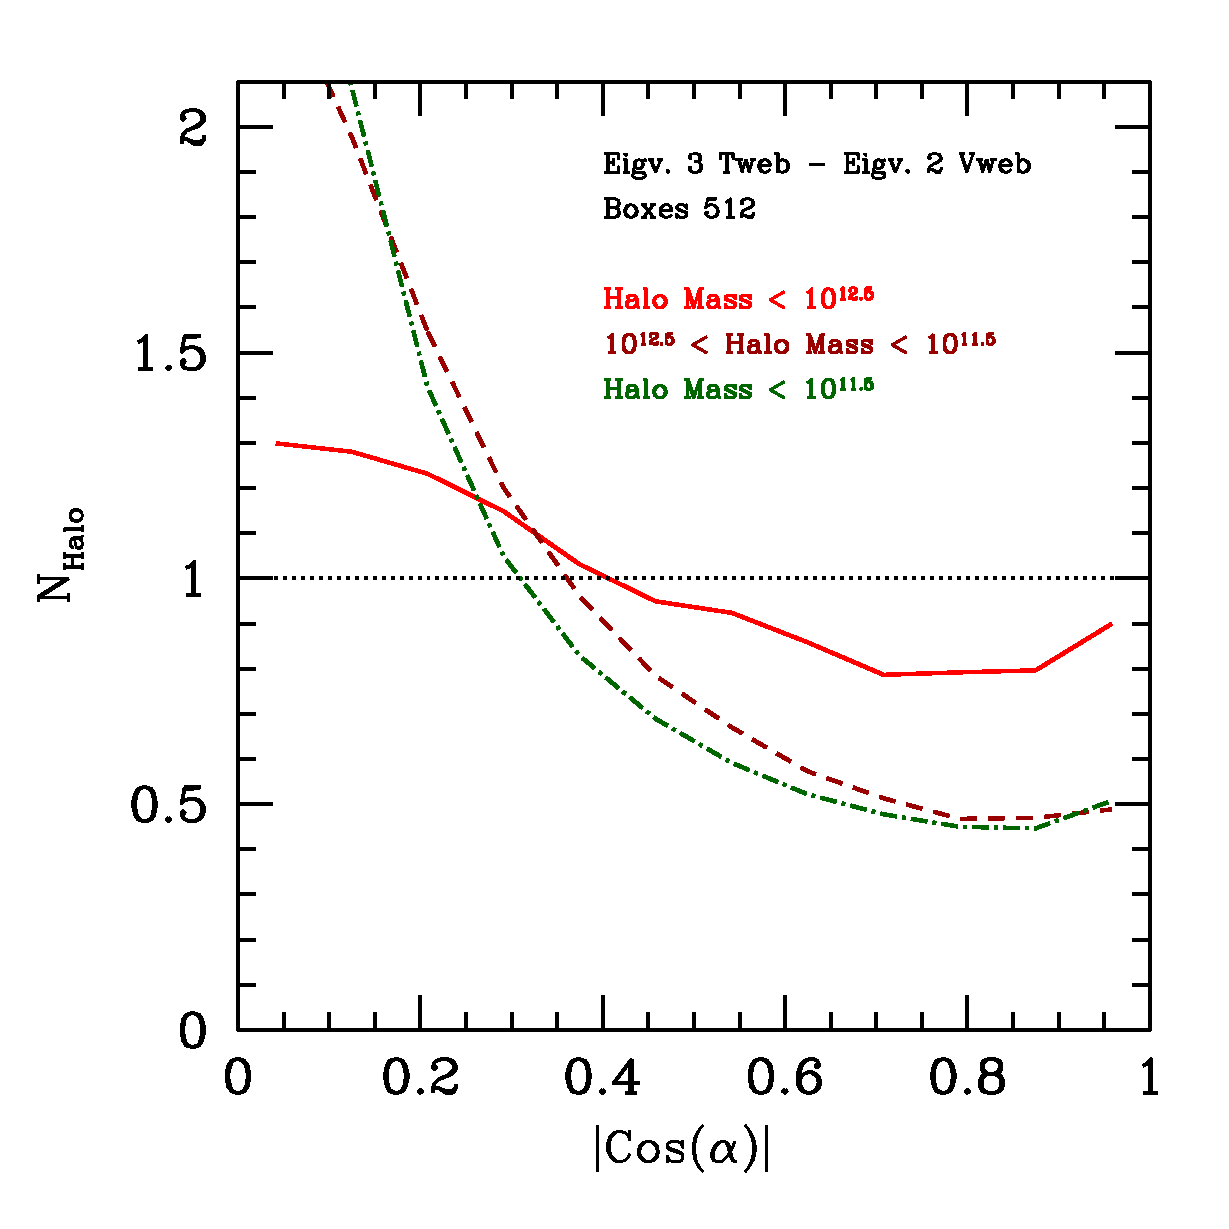
\includegraphics[width=0.30\textwidth]{../plot2/512/512_T3V2.ps}
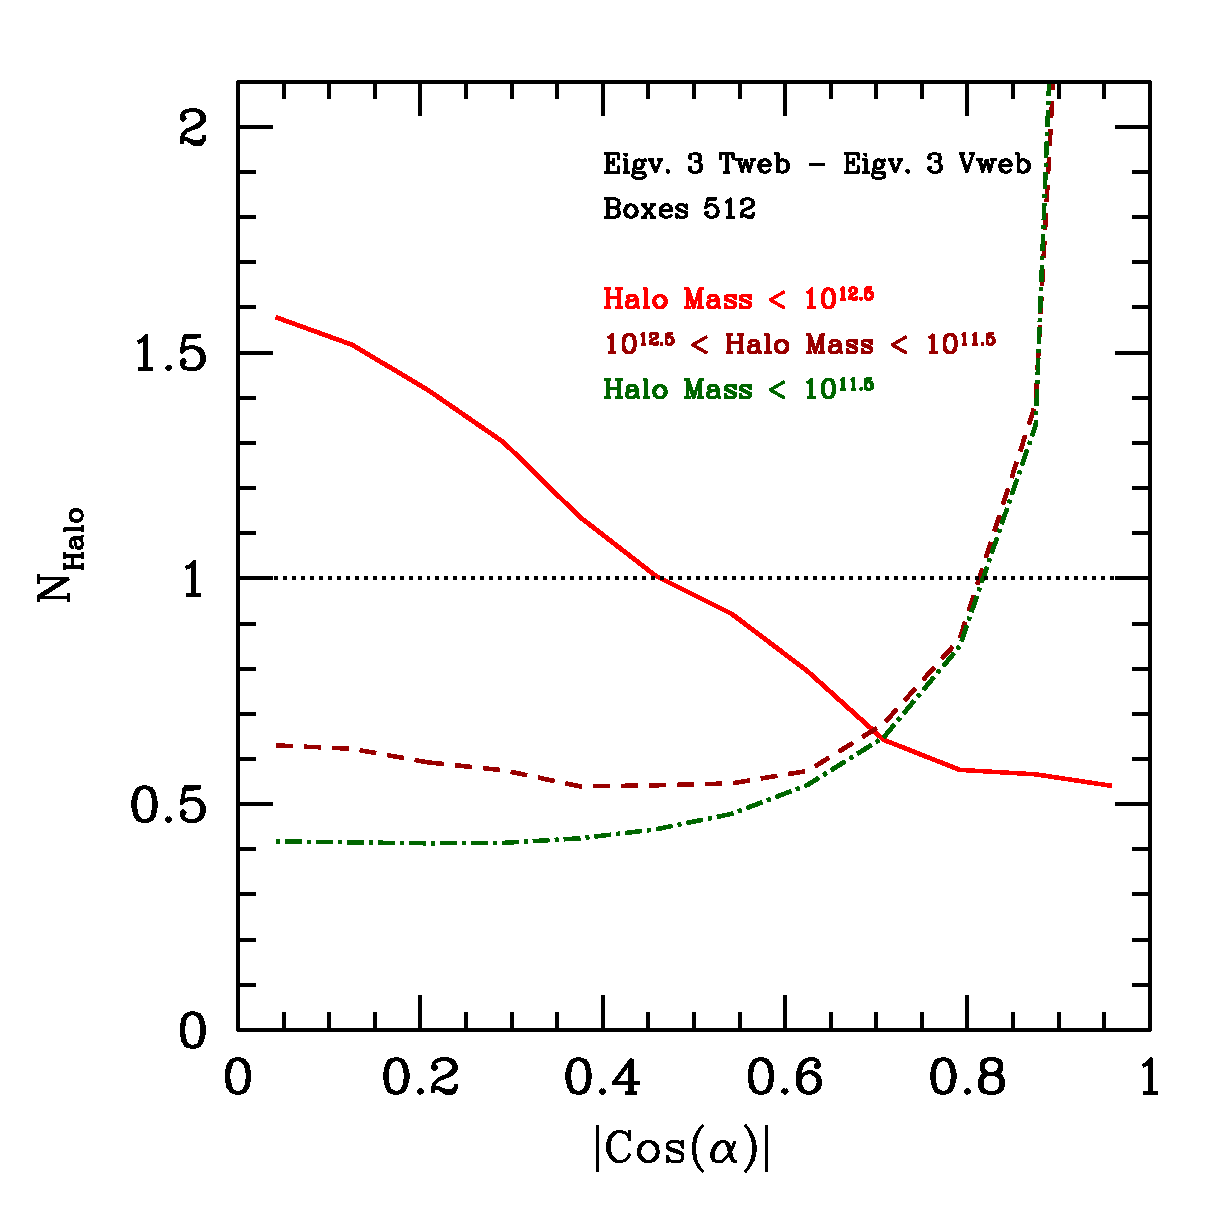
\includegraphics[width=0.30\textwidth]{../plot2/512/512_T3V3.ps}
\caption{Interweb alignment for $512^3$ grid resolution.}
\end{figure*}



\subsection{Shape Alignment}

\begin{figure*}
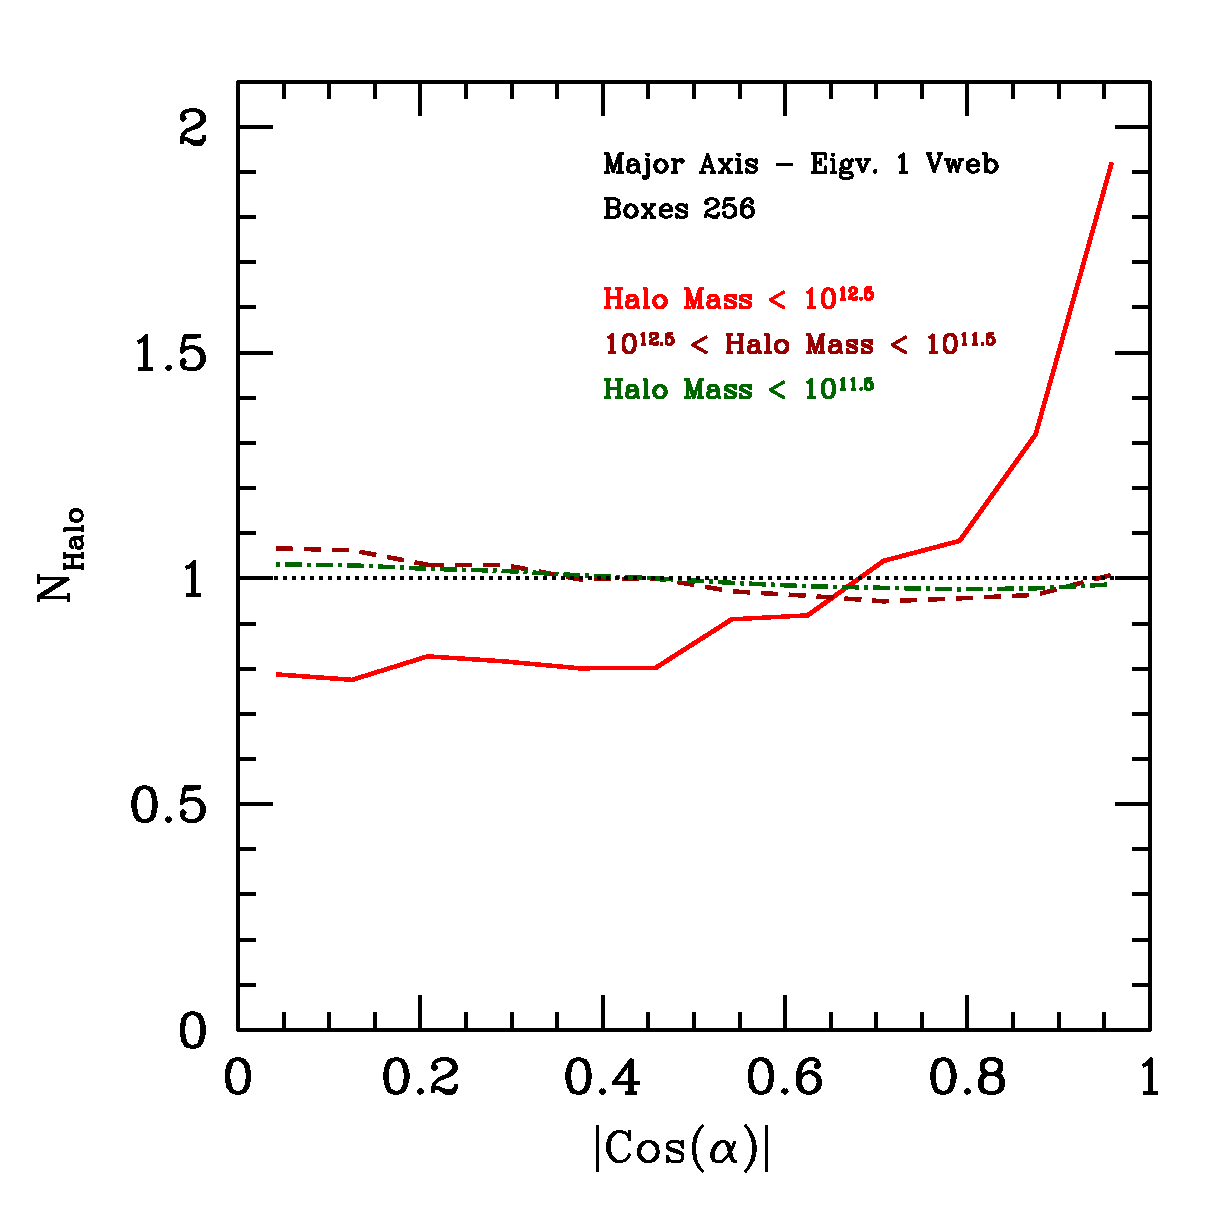
\includegraphics[width=0.30\textwidth]{../plot2/Ax1_VT/256_AX1_V1.ps}
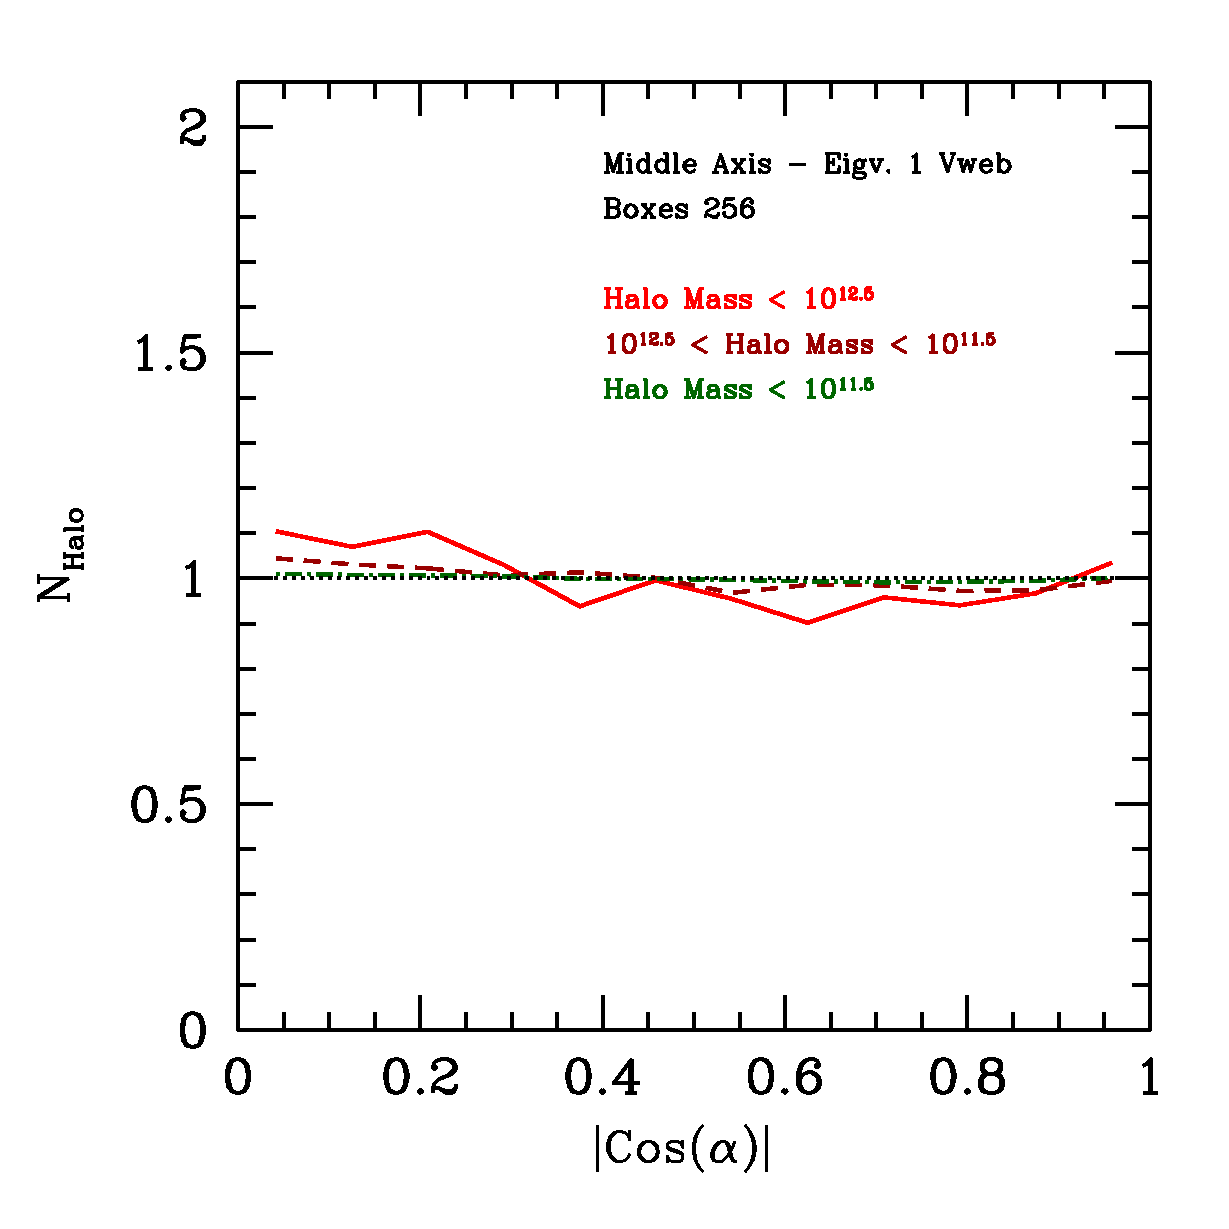
\includegraphics[width=0.30\textwidth]{../plot2/Ax2_VT/256_AX2_V1.ps}
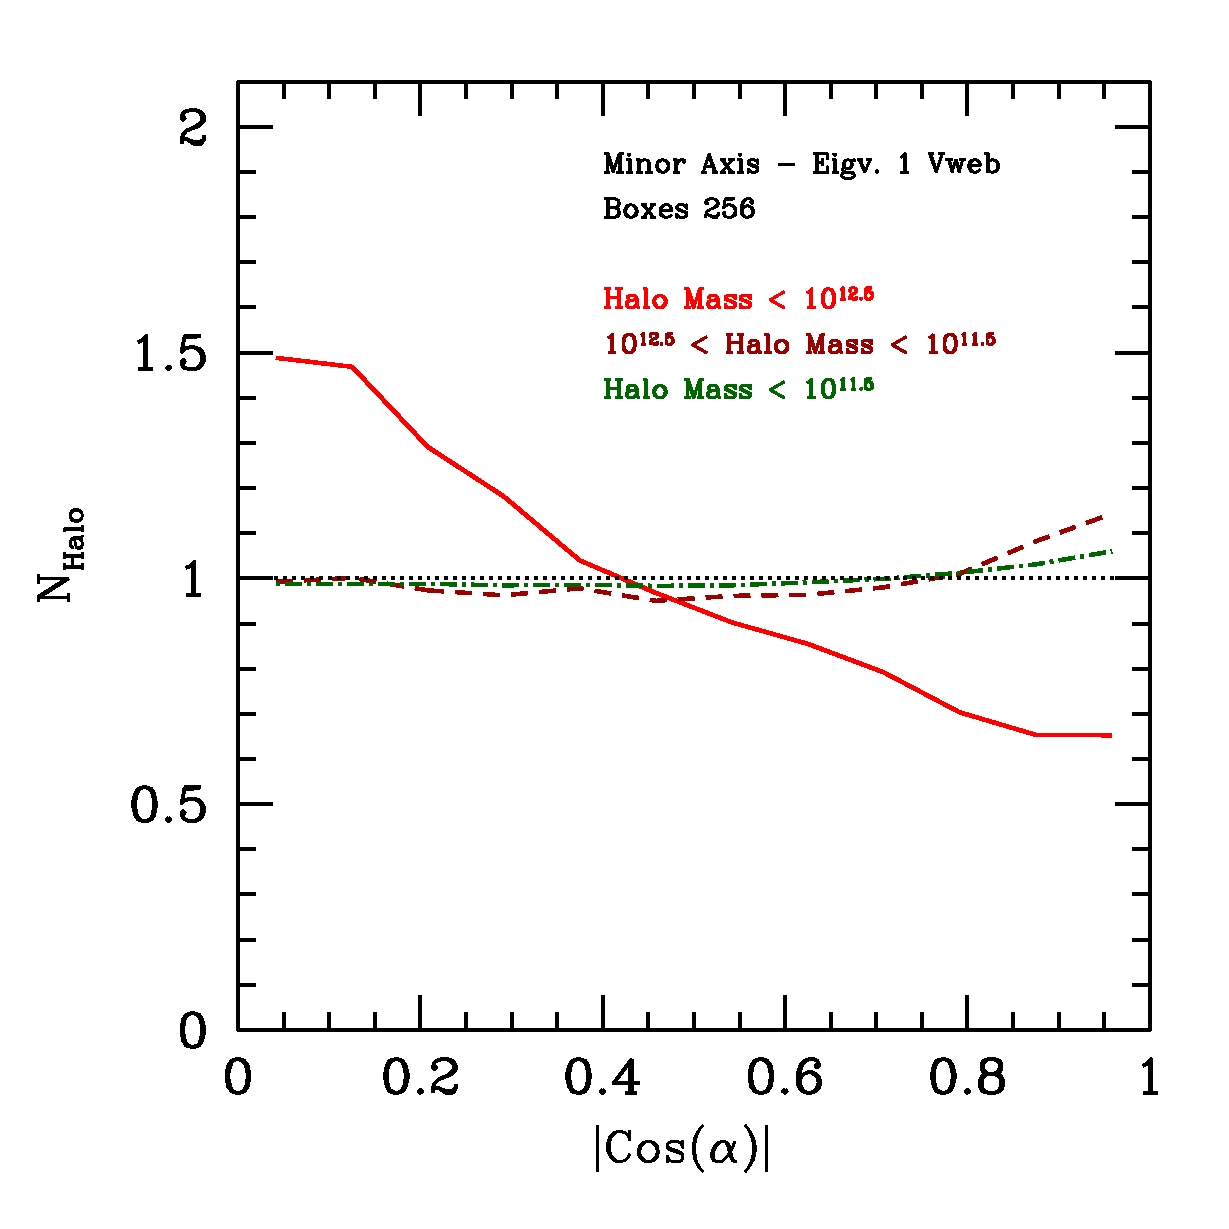
\includegraphics[width=0.30\textwidth]{../plot2/Ax3_VT/256_AX3_V1.ps}
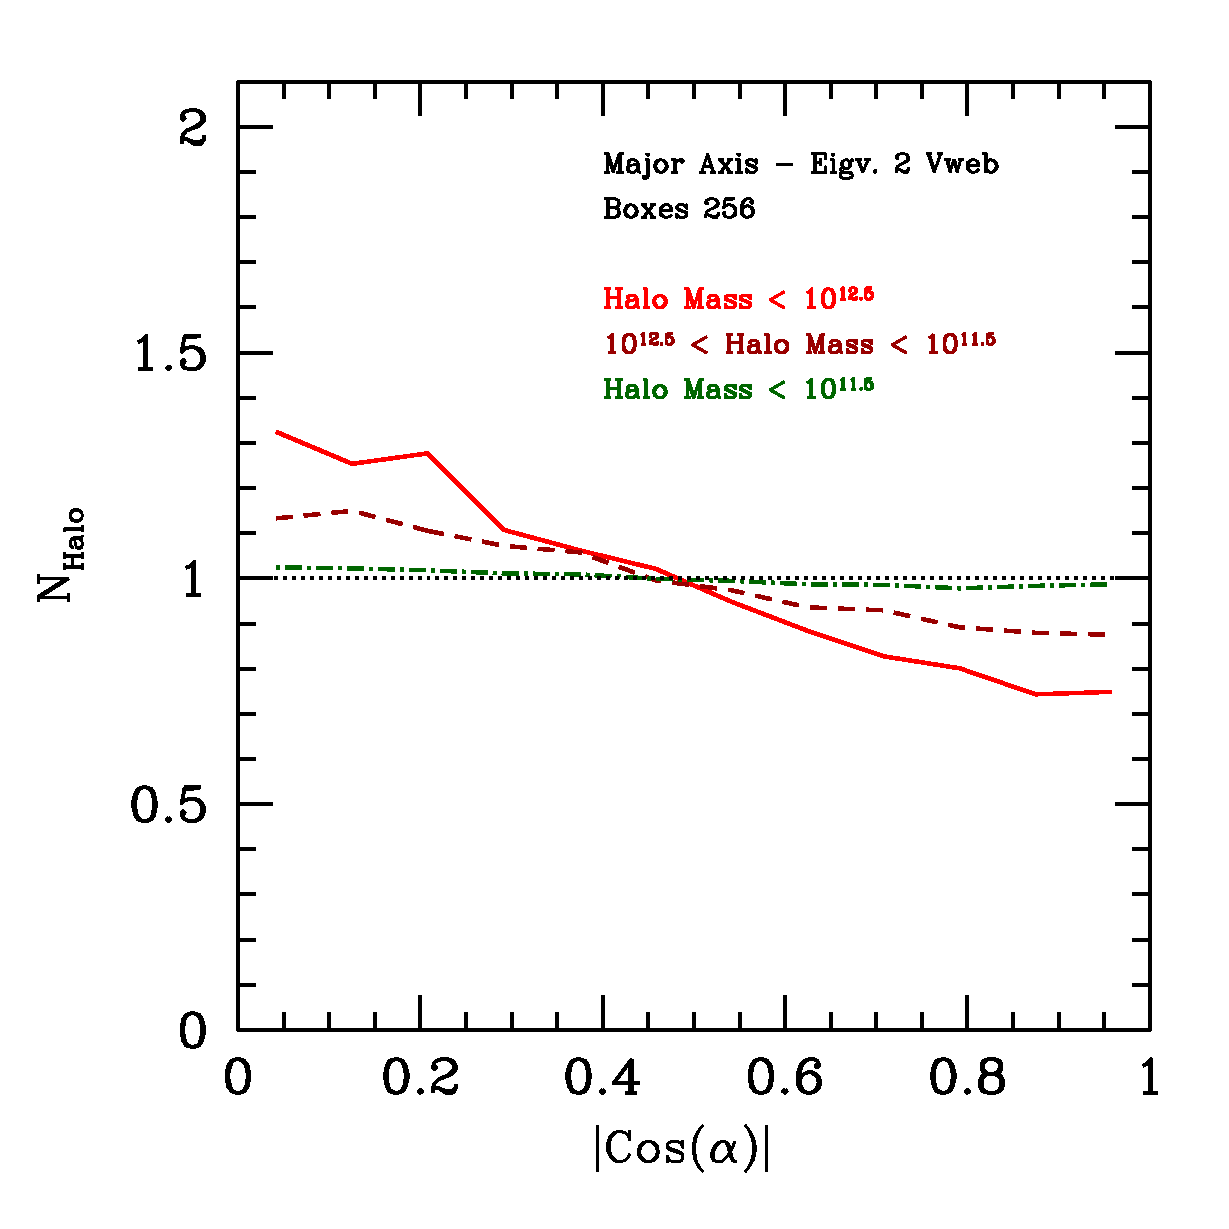
\includegraphics[width=0.30\textwidth]{../plot2/Ax1_VT/256_AX1_V2.ps}
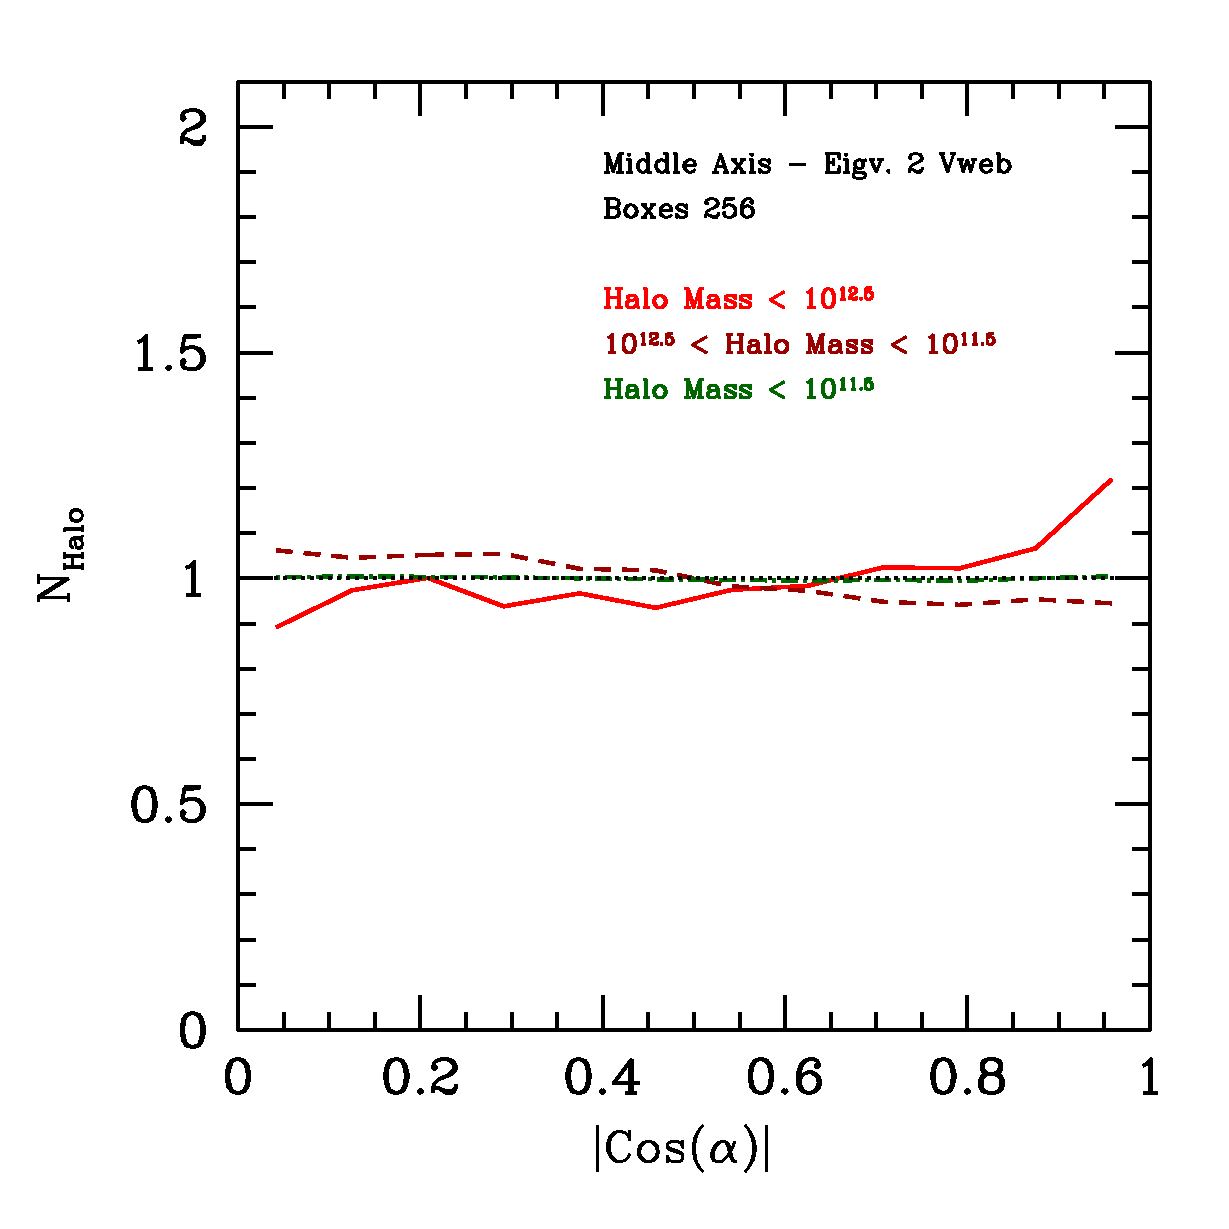
\includegraphics[width=0.30\textwidth]{../plot2/Ax2_VT/256_AX2_V2.ps}
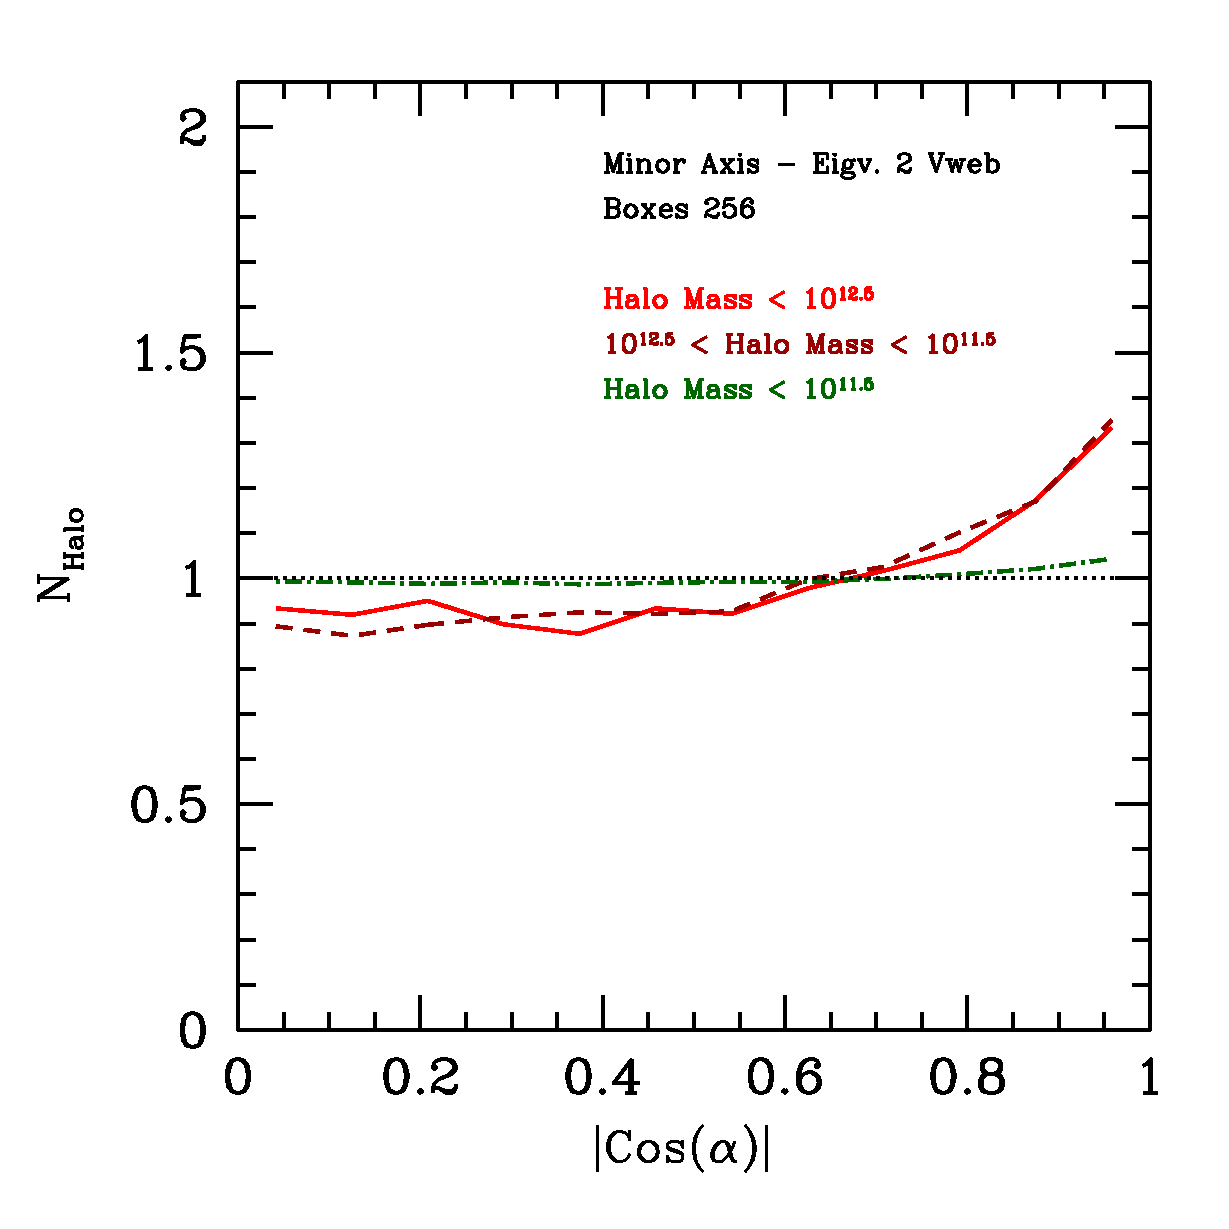
\includegraphics[width=0.30\textwidth]{../plot2/Ax3_VT/256_AX3_V2.ps}
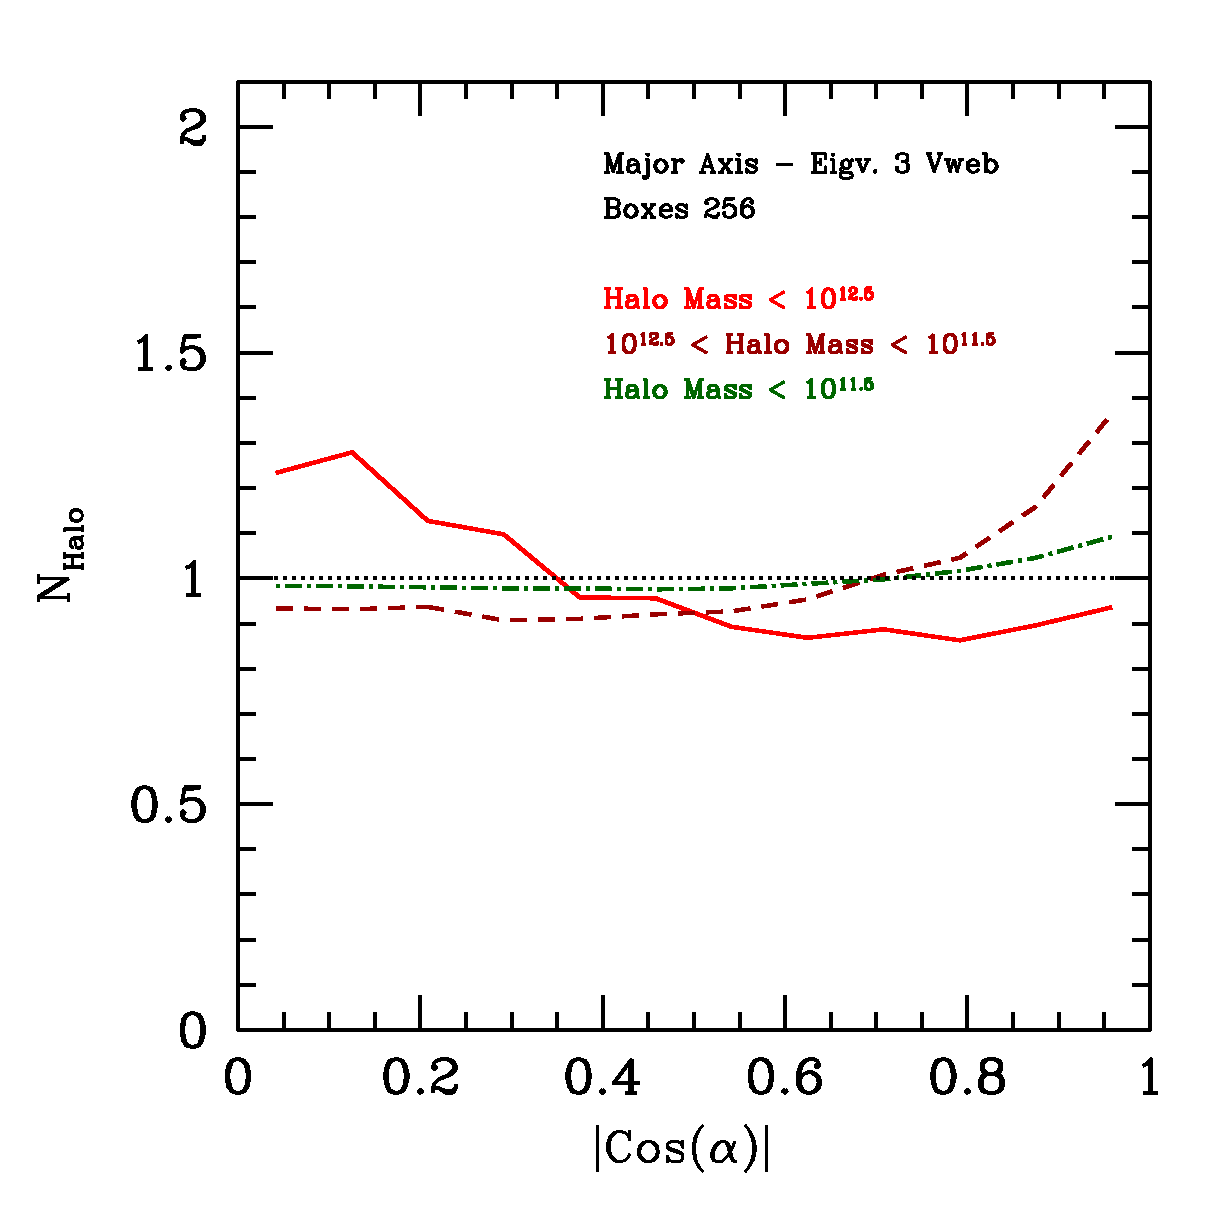
\includegraphics[width=0.30\textwidth]{../plot2/Ax1_VT/256_AX1_V3.ps}
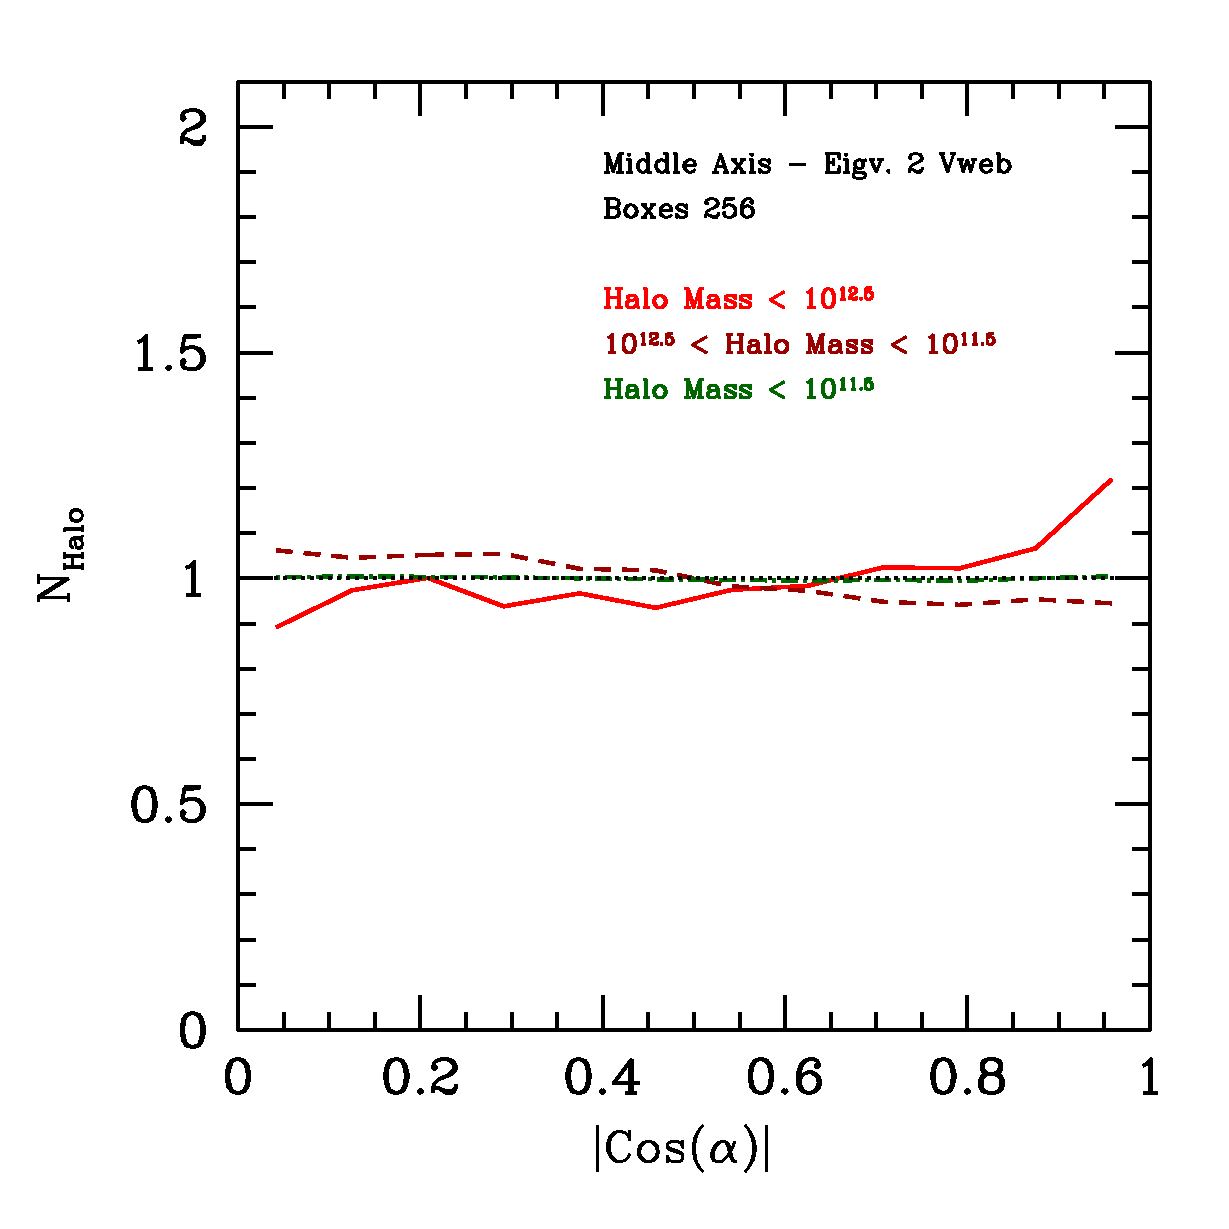
\includegraphics[width=0.30\textwidth]{../plot2/Ax2_VT/256_AX2_V2.ps}
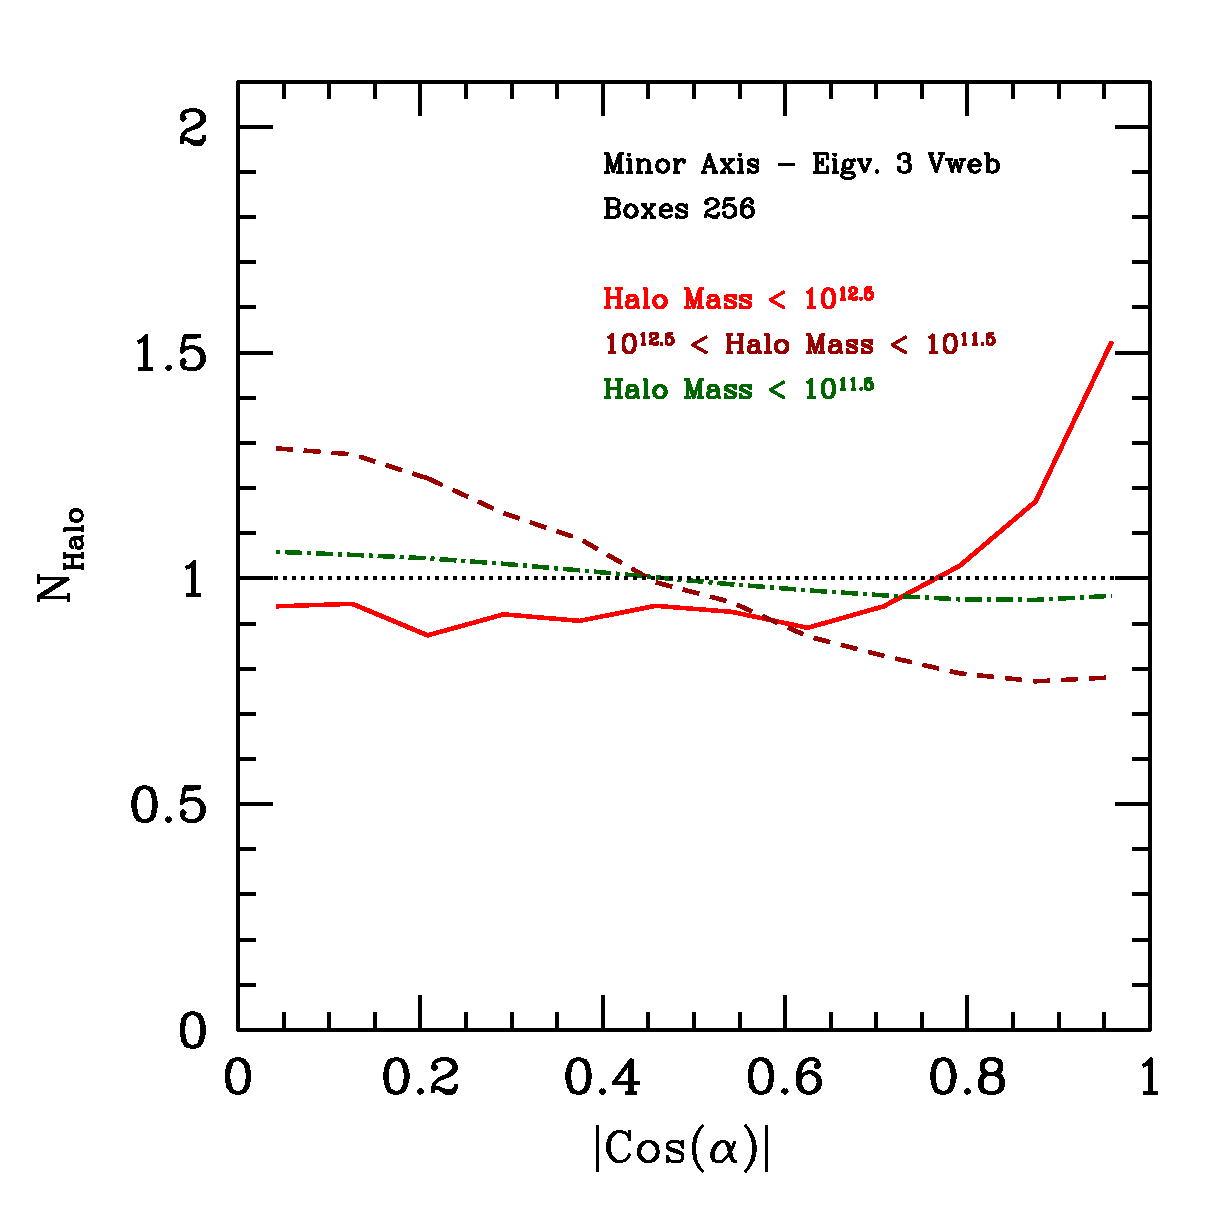
\includegraphics[width=0.30\textwidth]{../plot2/Ax3_VT/256_AX3_V3.ps}
\caption{Shape alignment for the vweb at $256^3$ resolution.}
\end{figure*}

\begin{figure*}
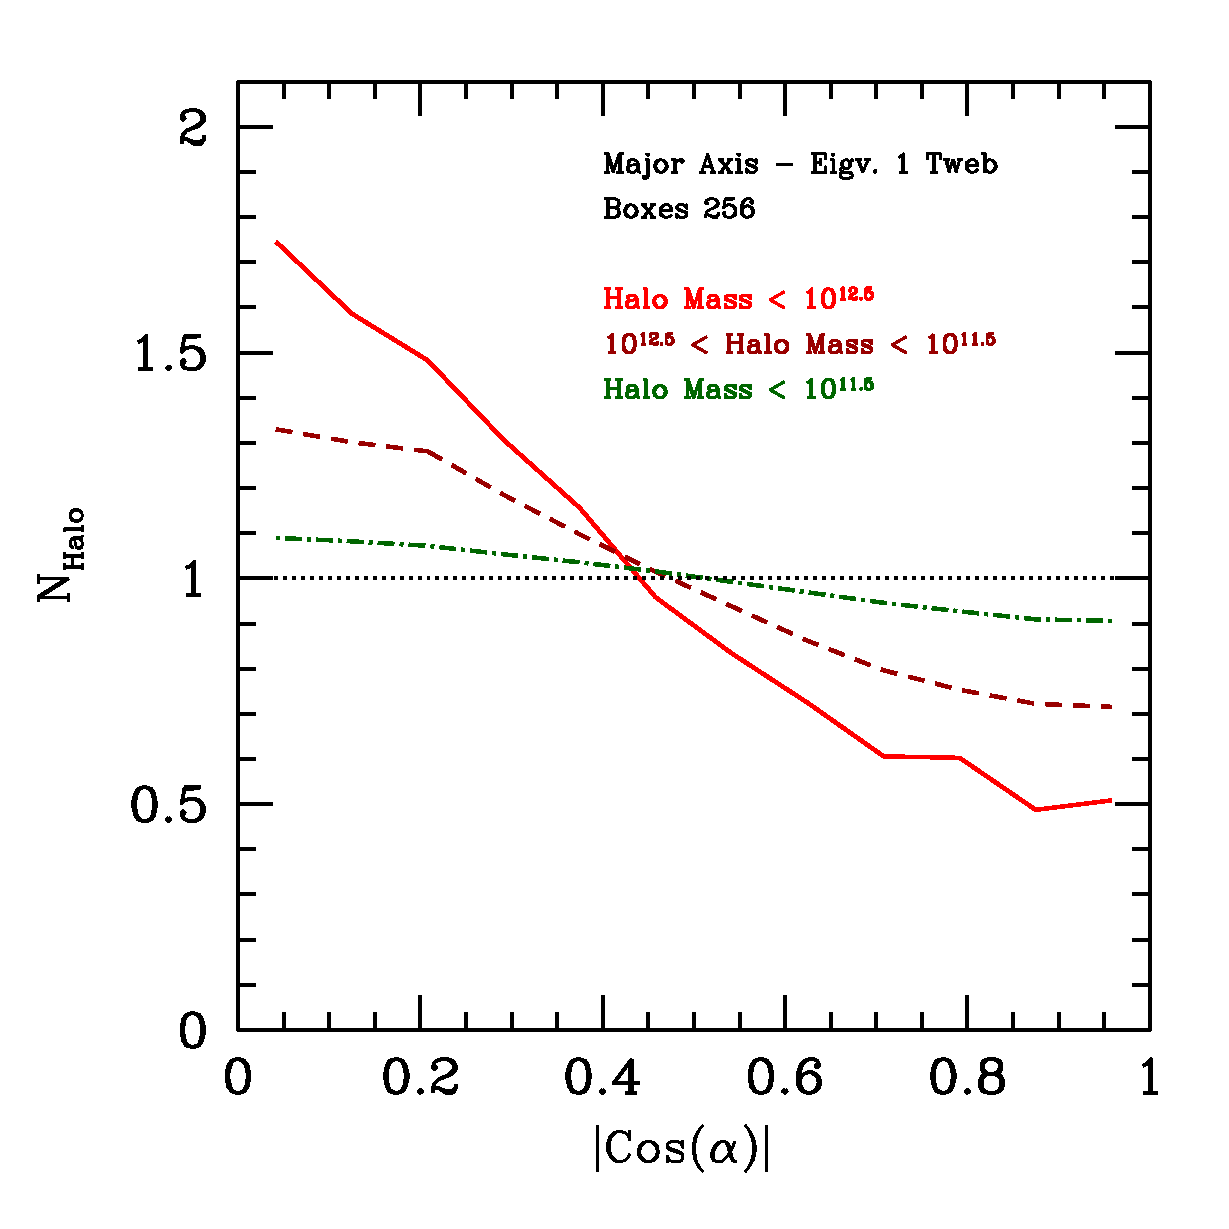
\includegraphics[width=0.30\textwidth]{../plot2/Ax1_VT/256_AX1_T1.ps}
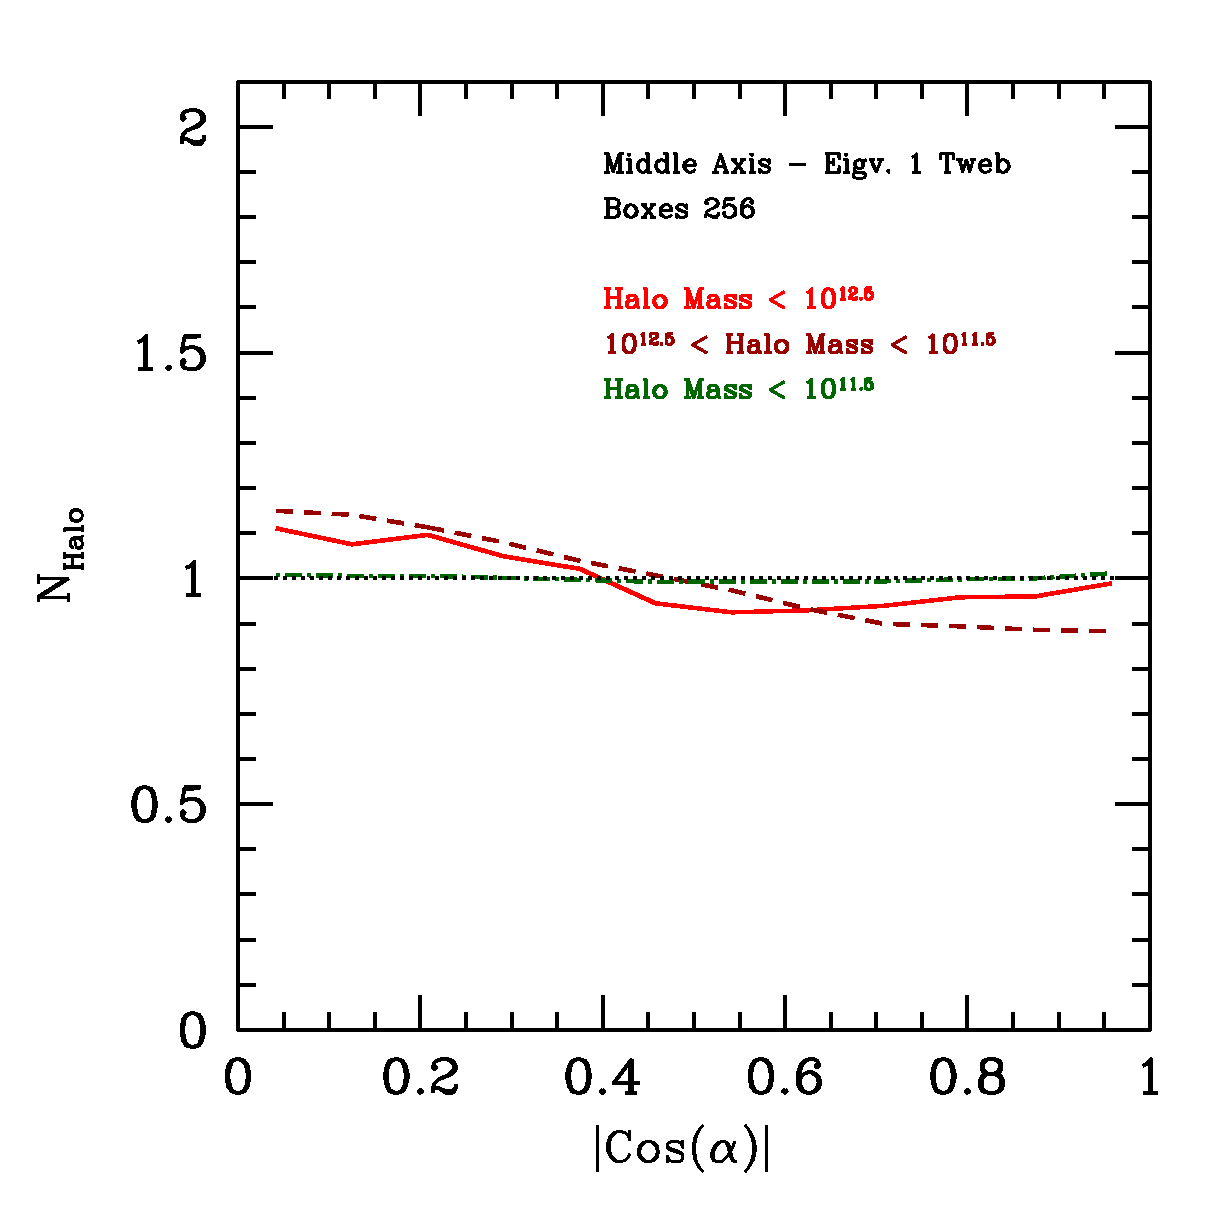
\includegraphics[width=0.30\textwidth]{../plot2/Ax2_VT/256_AX2_T1.ps}
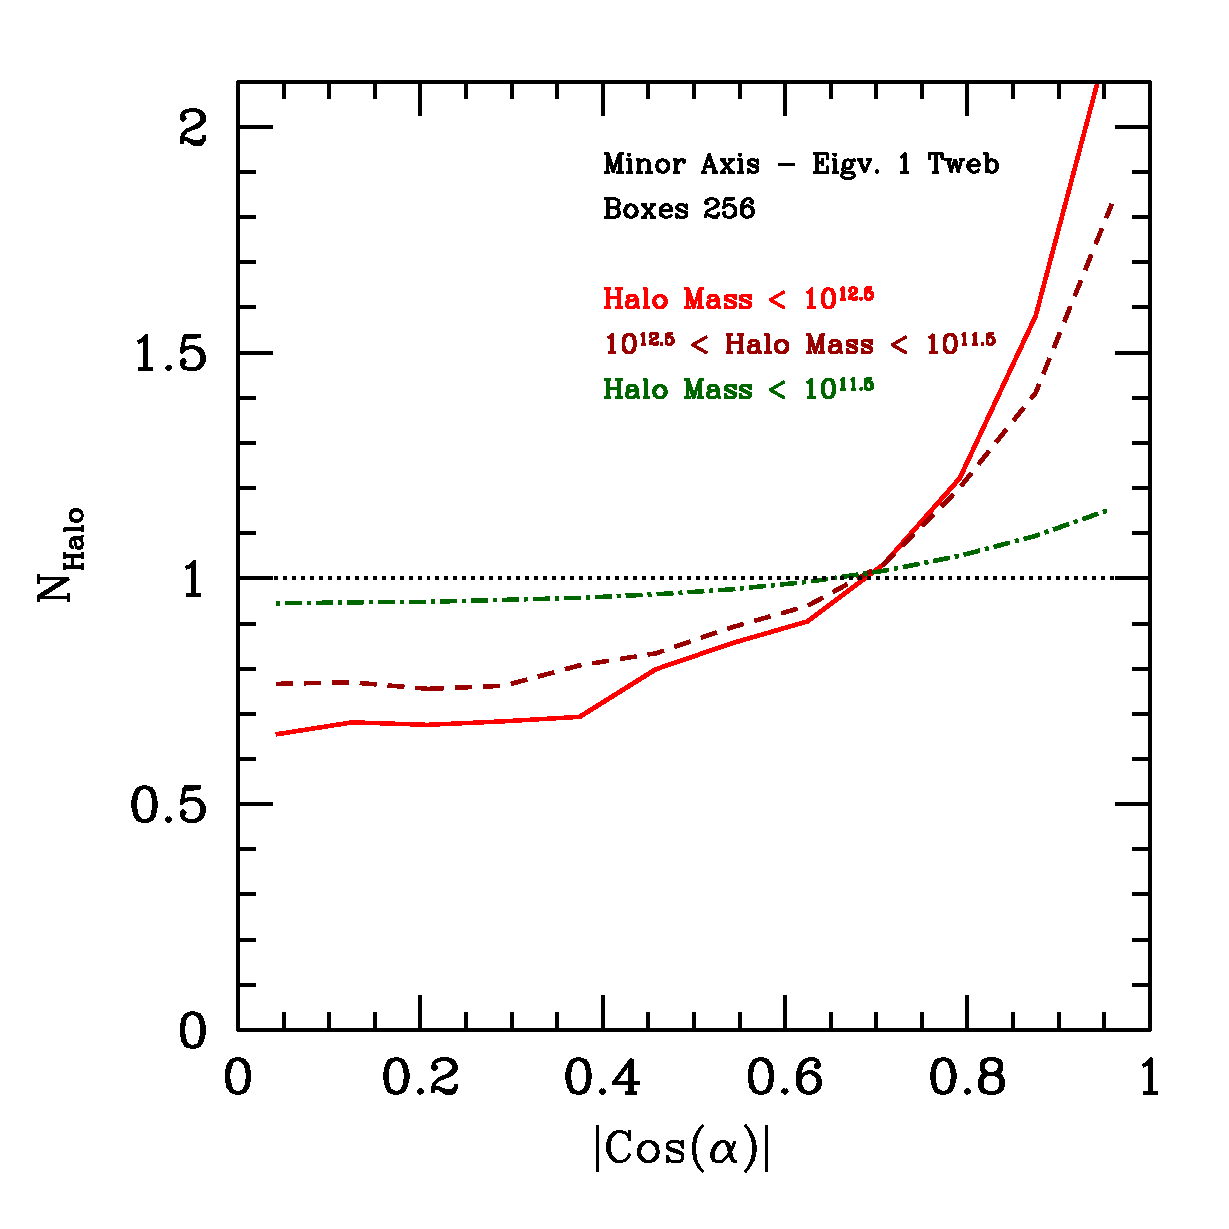
\includegraphics[width=0.30\textwidth]{../plot2/Ax3_VT/256_AX3_T1.ps}
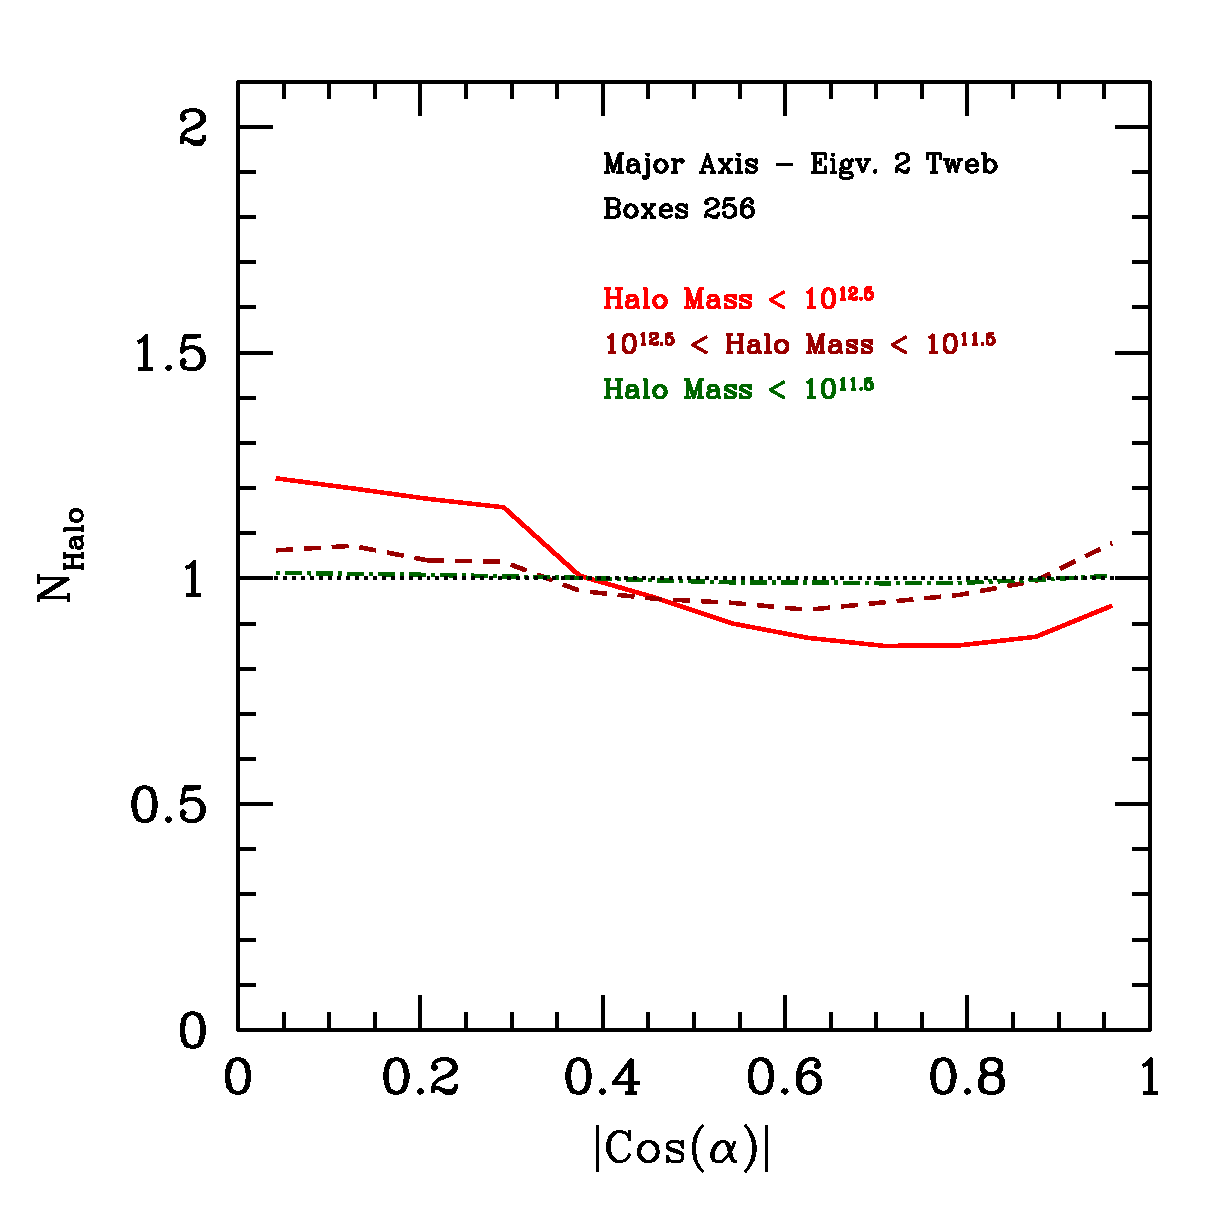
\includegraphics[width=0.30\textwidth]{../plot2/Ax1_VT/256_AX1_T2.ps}
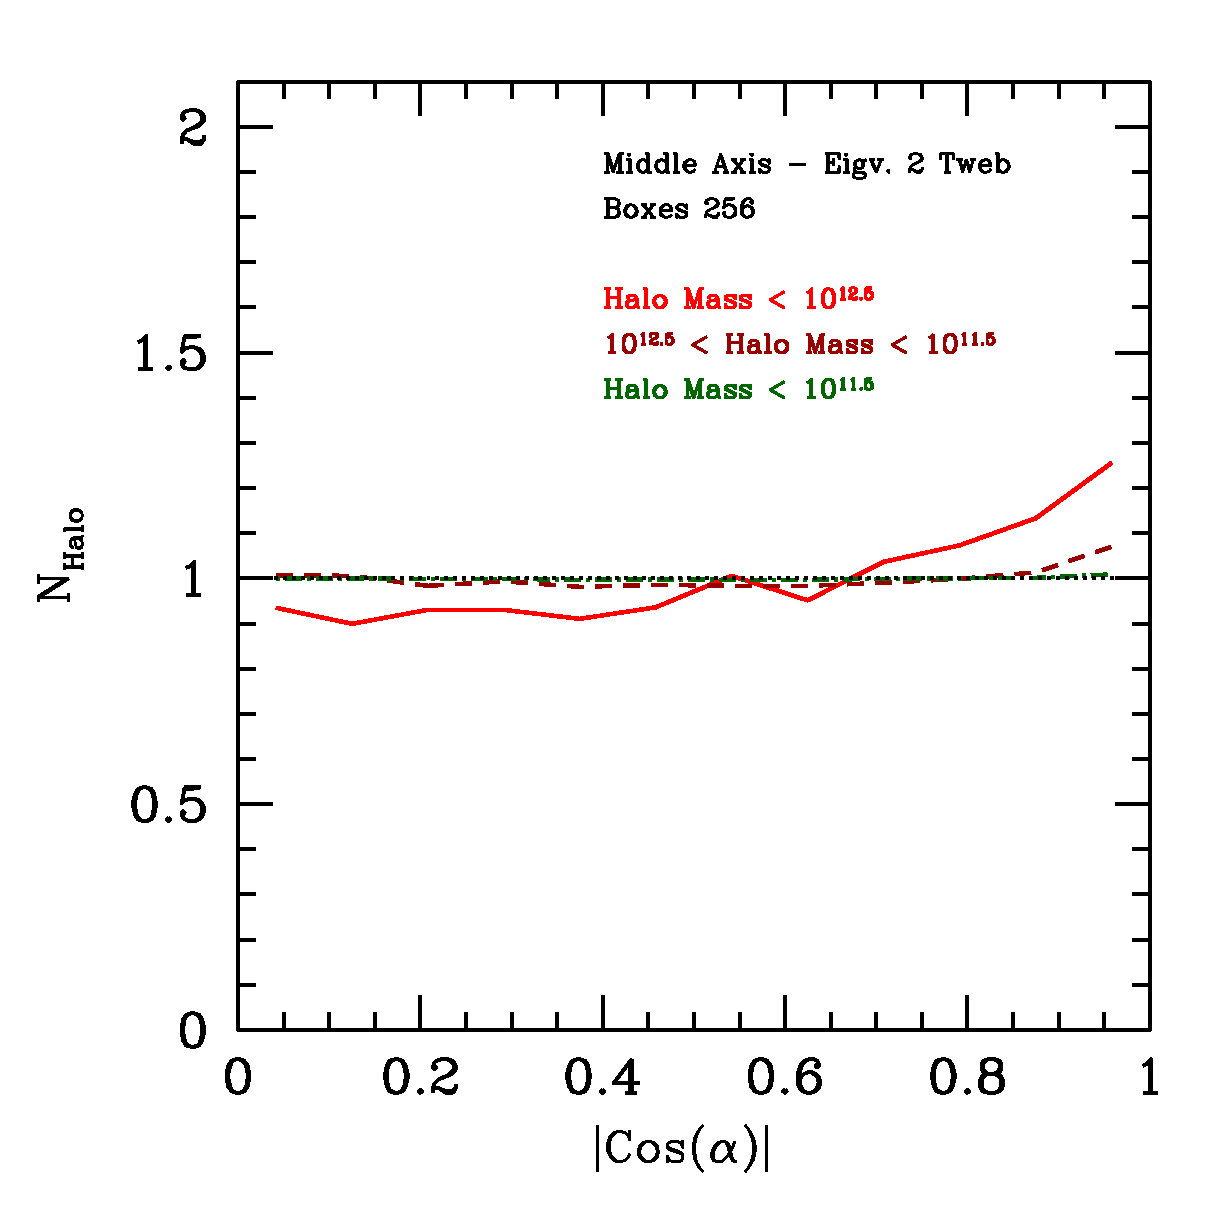
\includegraphics[width=0.30\textwidth]{../plot2/Ax2_VT/256_AX2_T2.ps}
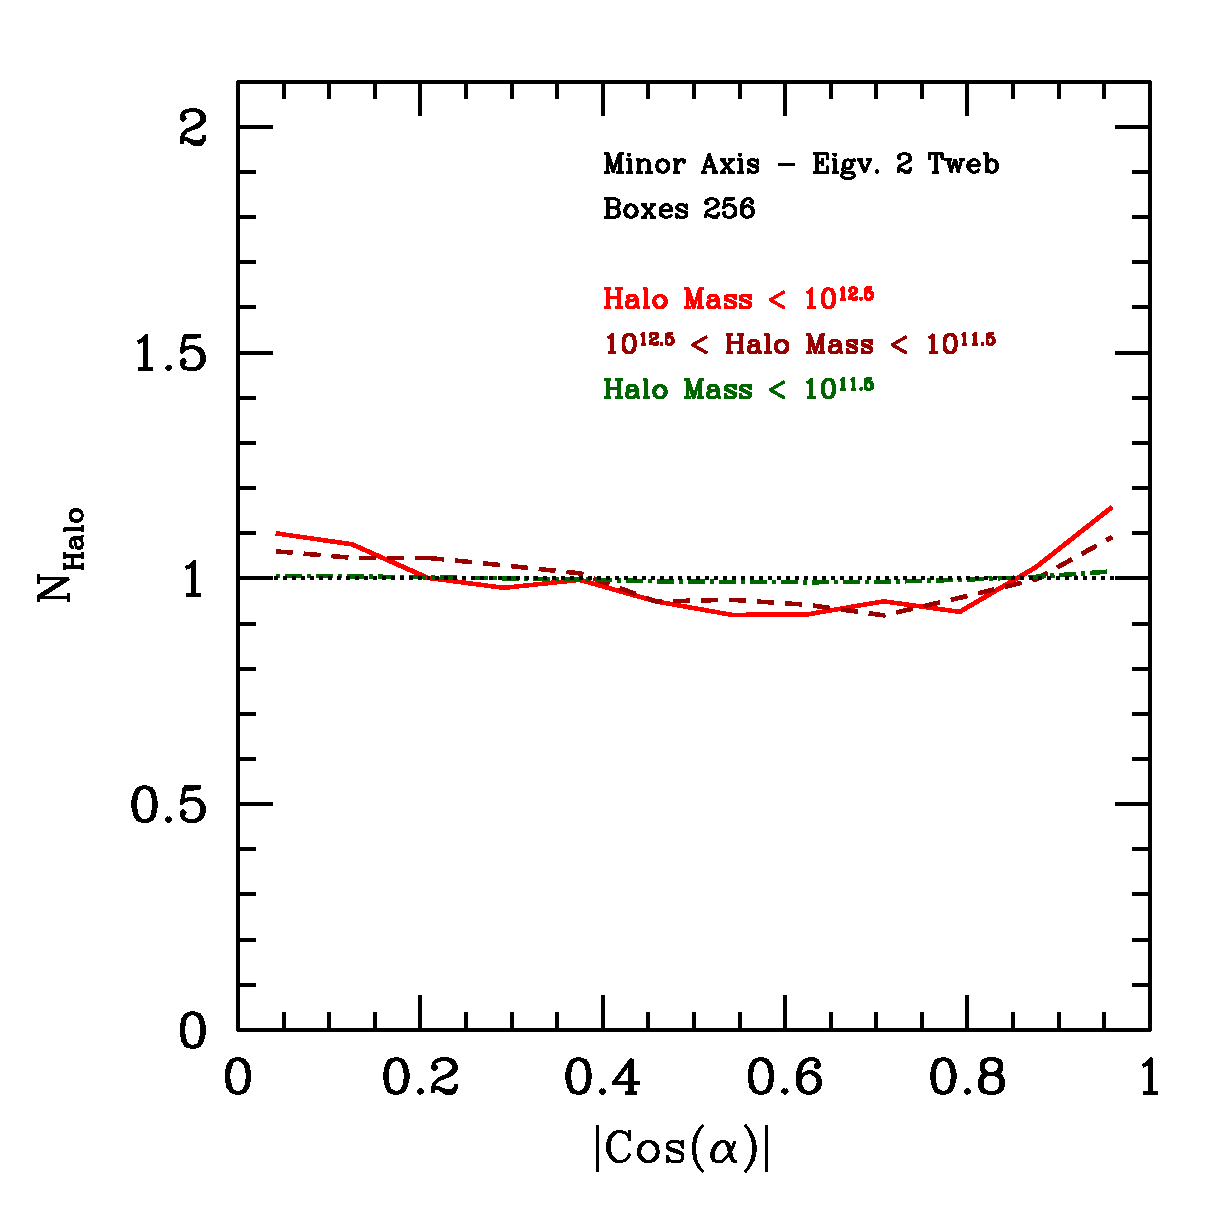
\includegraphics[width=0.30\textwidth]{../plot2/Ax3_VT/256_AX3_T2.ps}
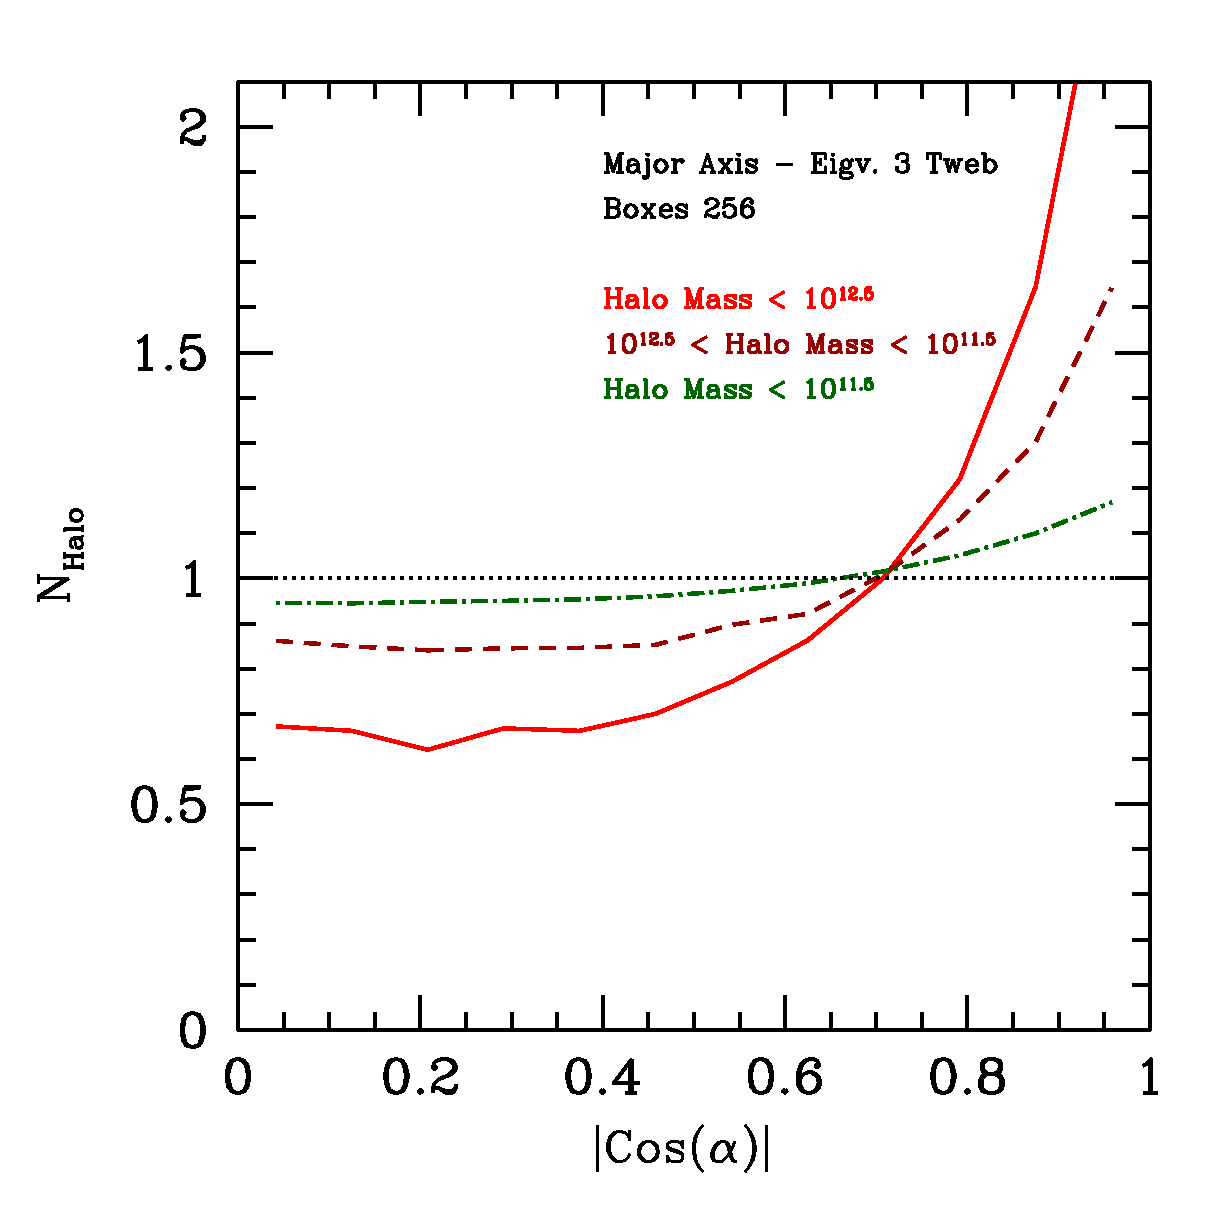
\includegraphics[width=0.30\textwidth]{../plot2/Ax1_VT/256_AX1_T3.ps}
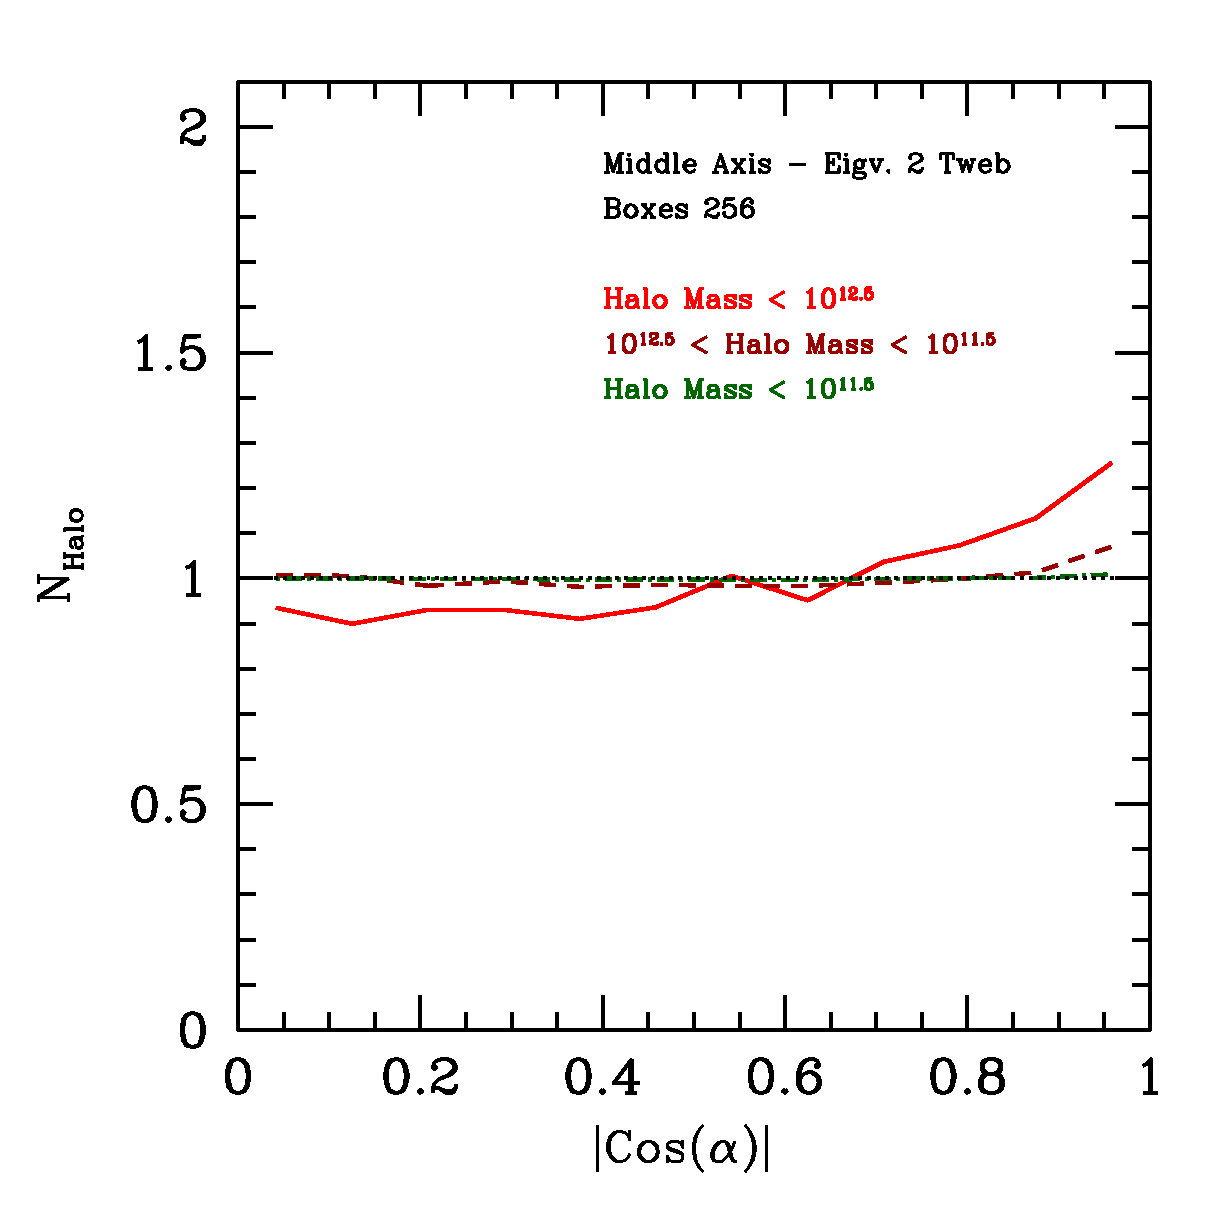
\includegraphics[width=0.30\textwidth]{../plot2/Ax2_VT/256_AX2_T2.ps}
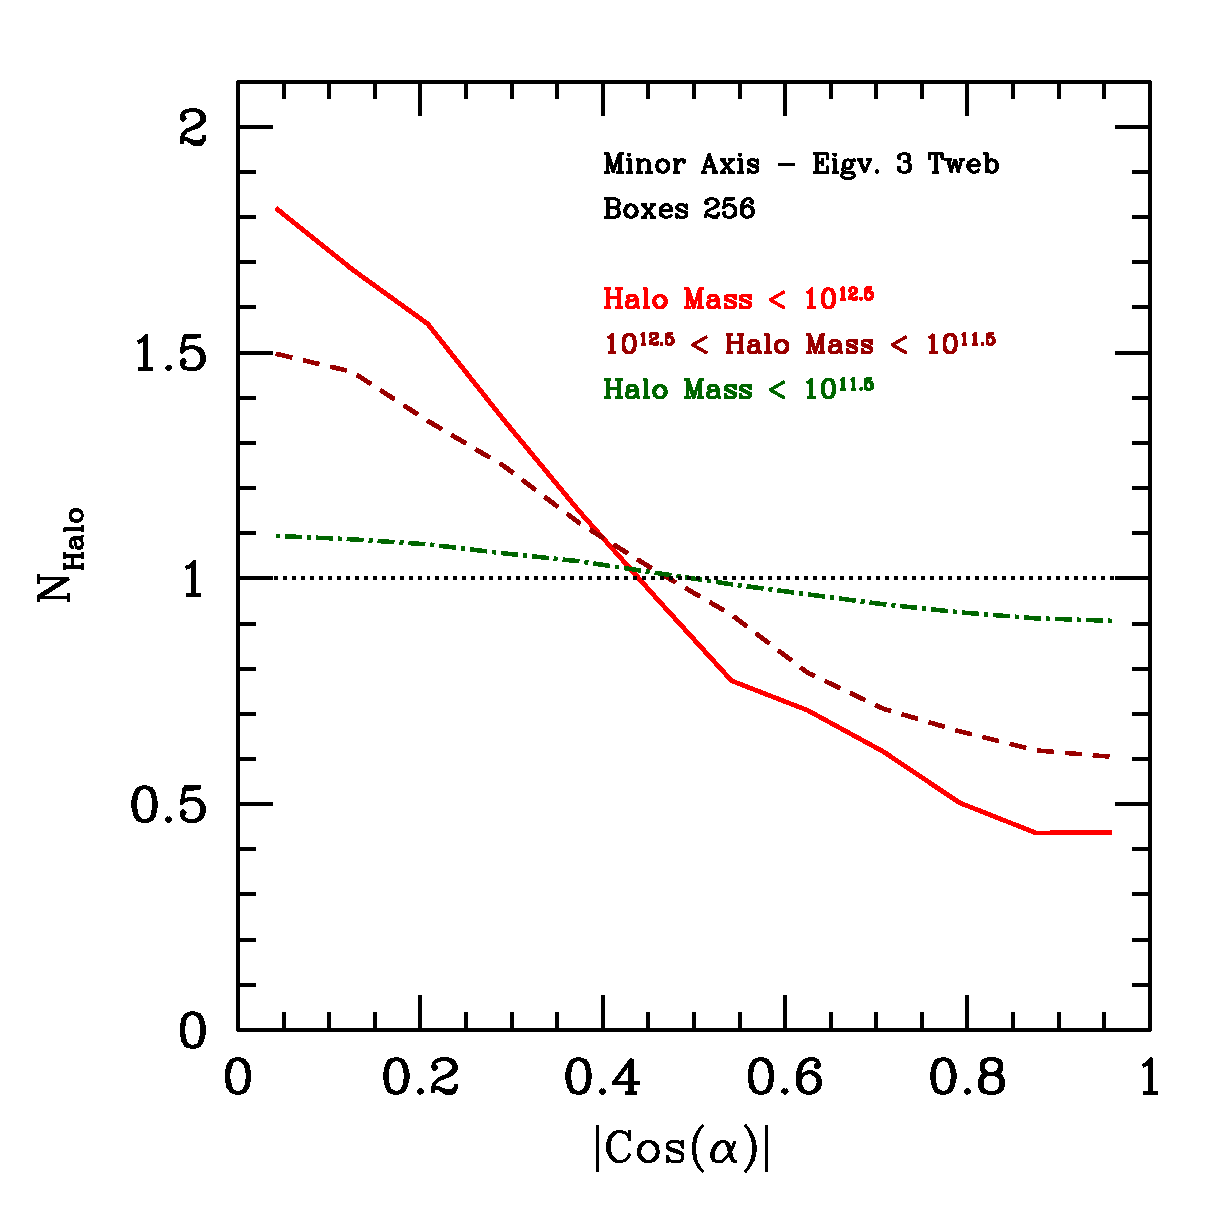
\includegraphics[width=0.30\textwidth]{../plot2/Ax3_VT/256_AX3_T3.ps}
\caption{Shape alignment for the tweb at $256^3$ resolution.}
\end{figure*}


\begin{figure*}
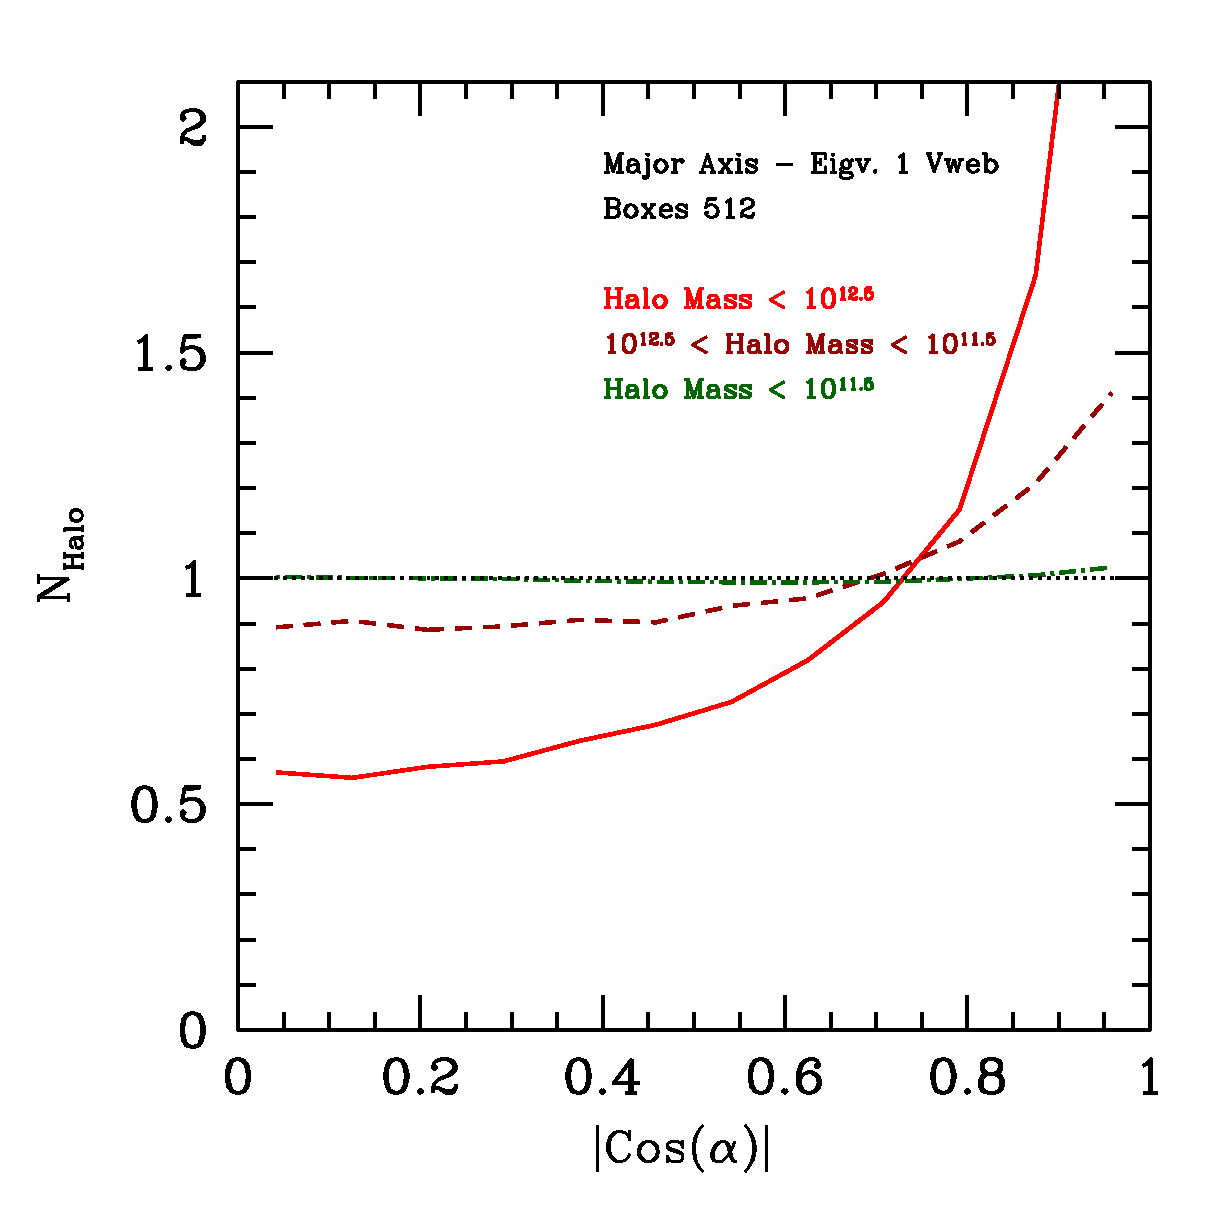
\includegraphics[width=0.30\textwidth]{../plot2/Ax1_VT/512_AX1_V1.ps}
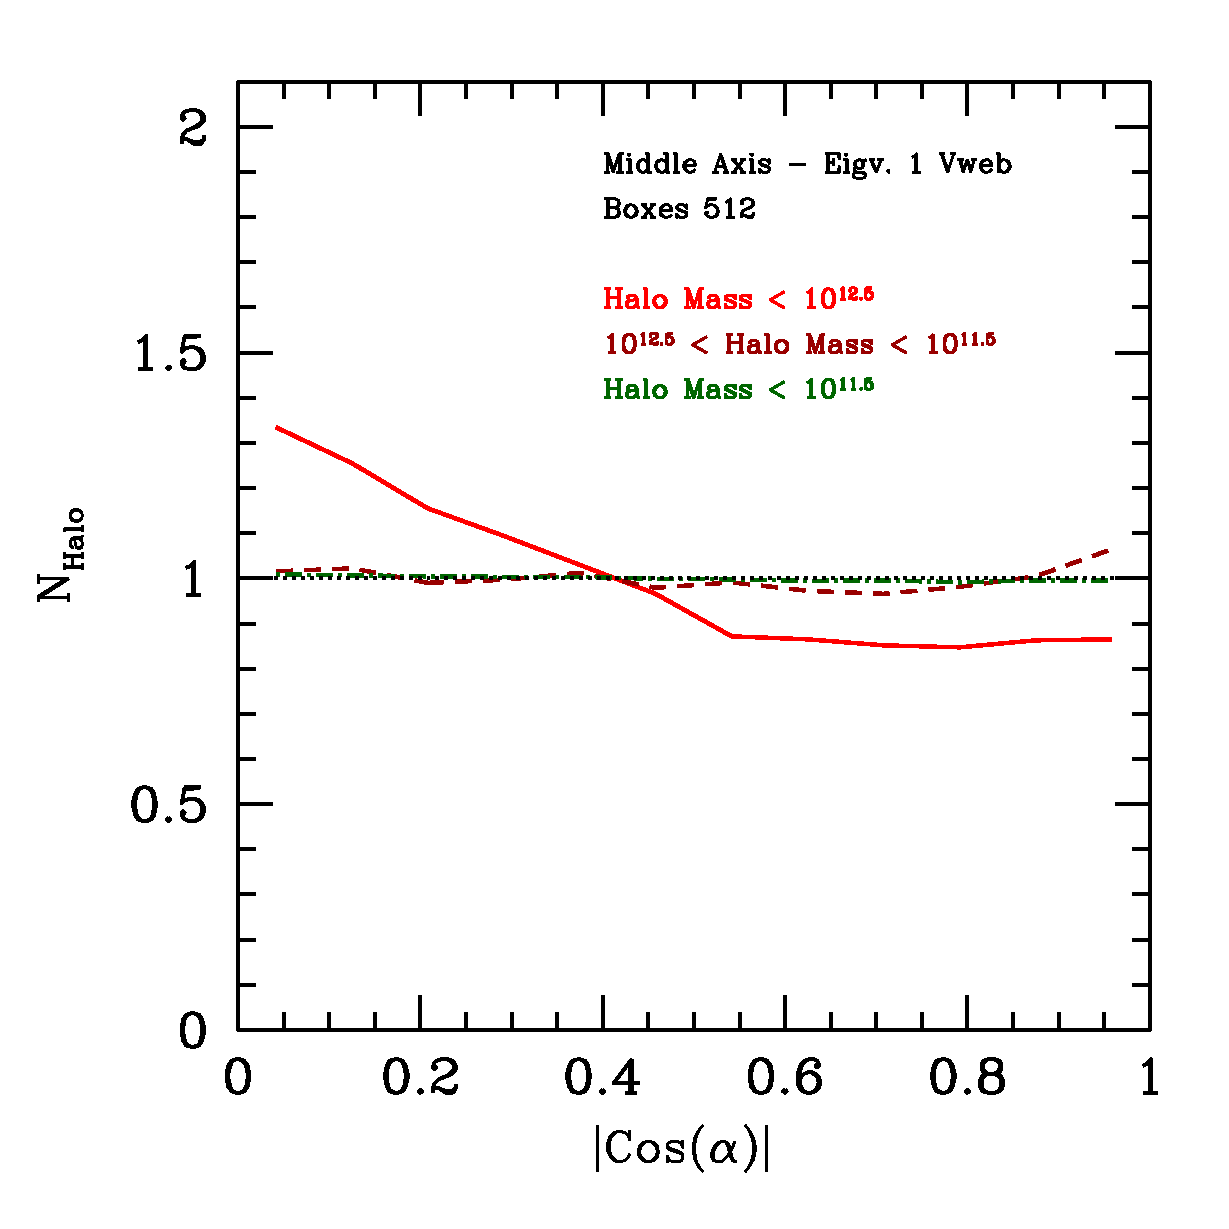
\includegraphics[width=0.30\textwidth]{../plot2/Ax2_VT/512_AX2_V1.ps}
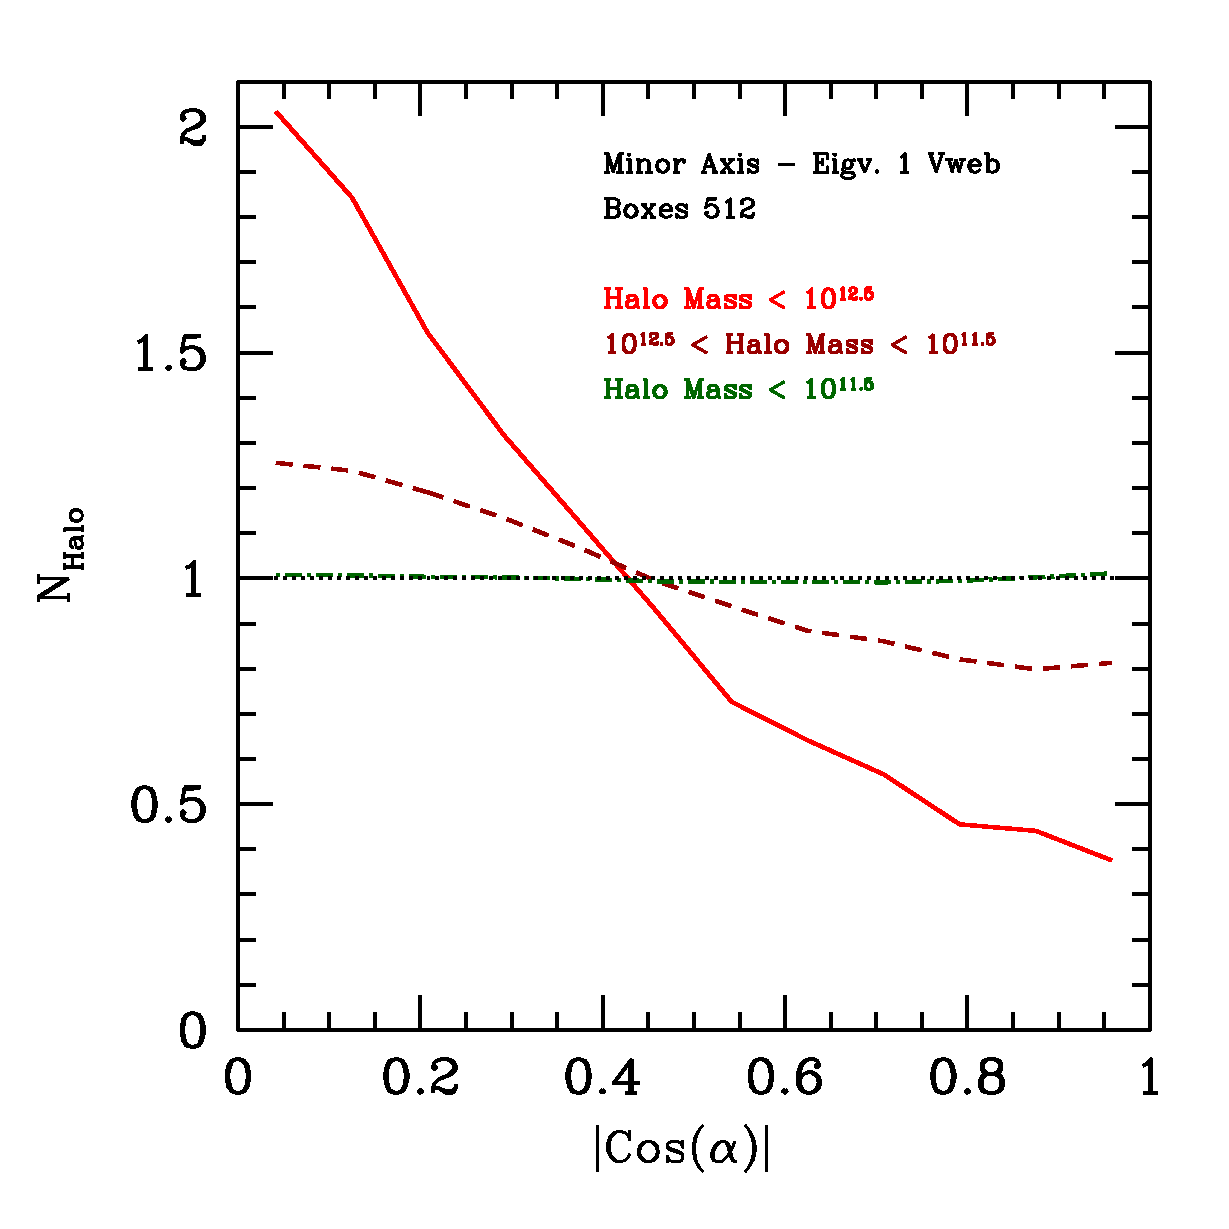
\includegraphics[width=0.30\textwidth]{../plot2/Ax3_VT/512_AX3_V1.ps}
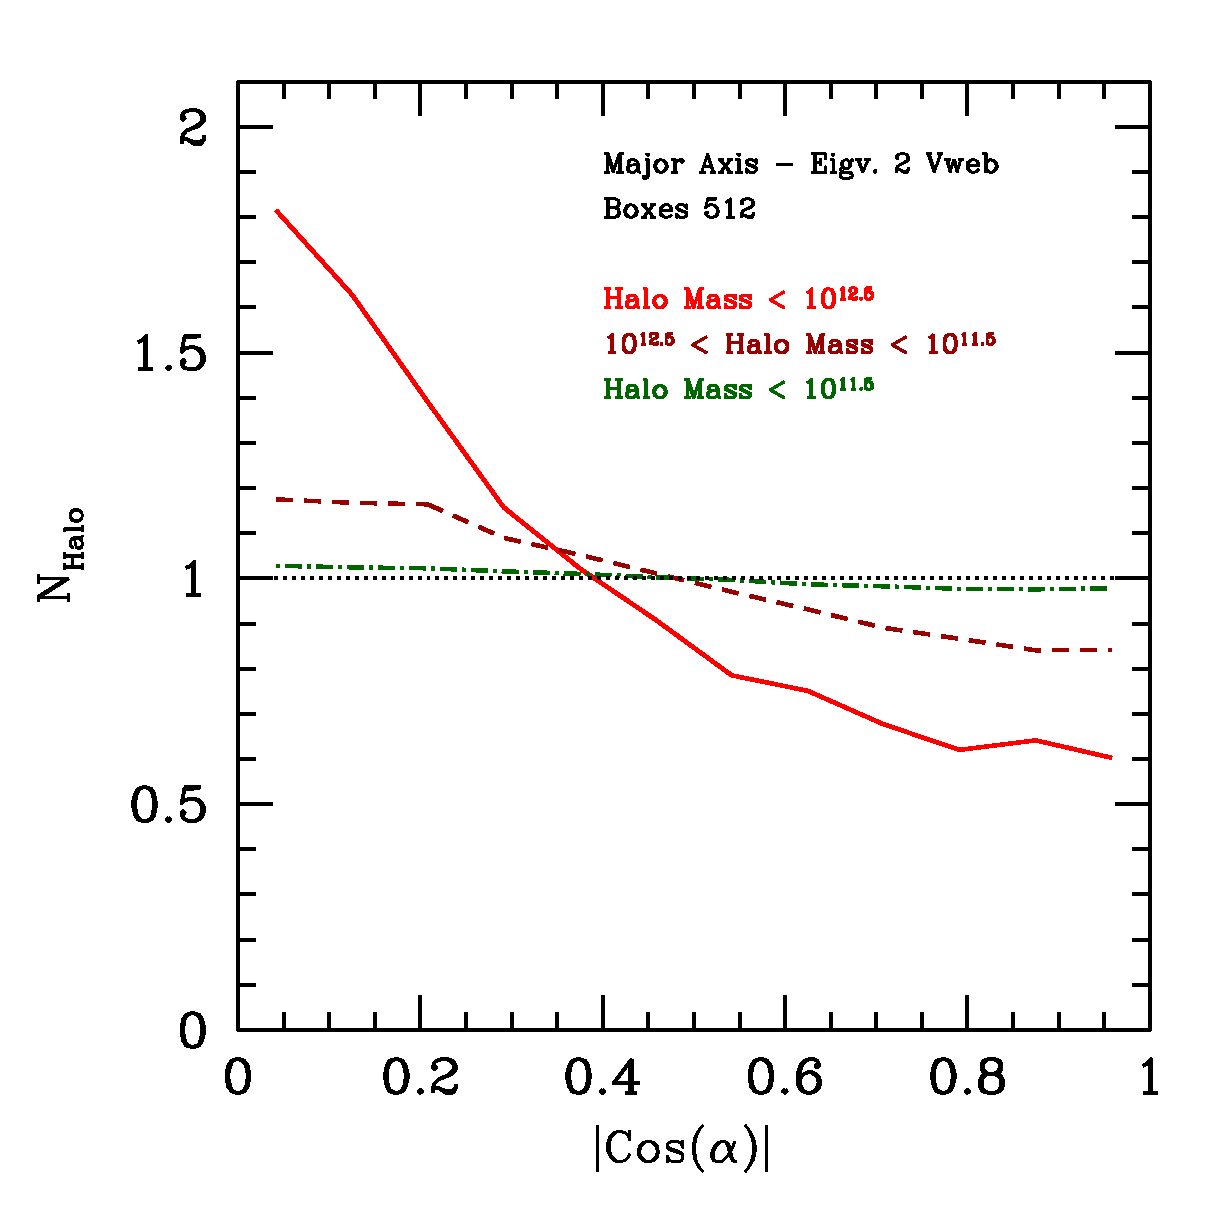
\includegraphics[width=0.30\textwidth]{../plot2/Ax1_VT/512_AX1_V2.ps}
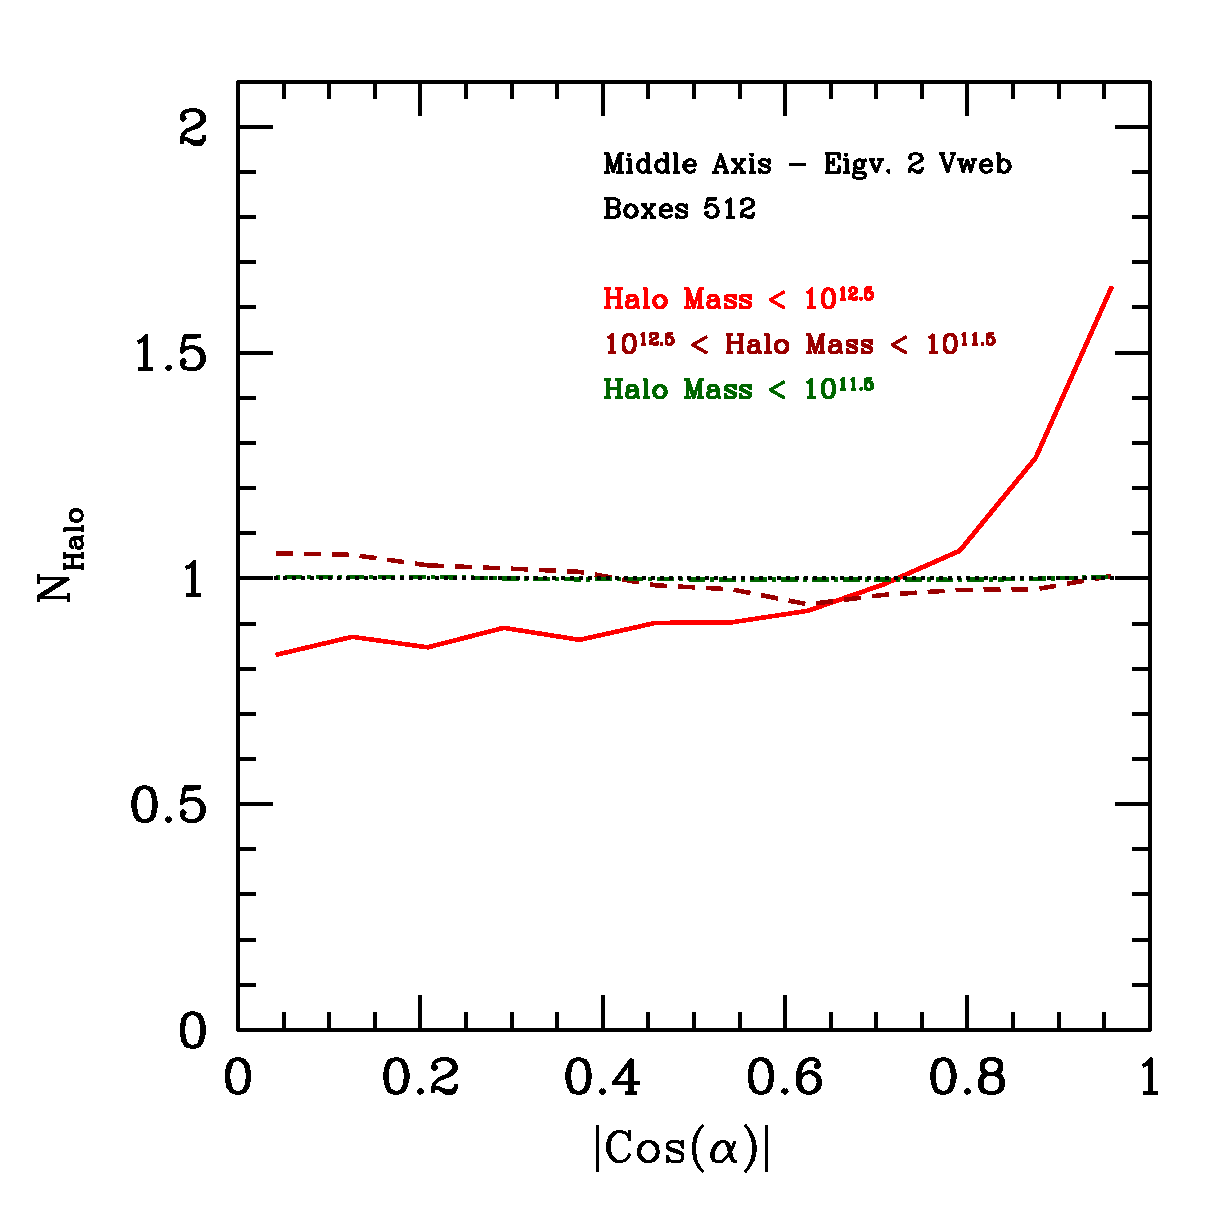
\includegraphics[width=0.30\textwidth]{../plot2/Ax2_VT/512_AX2_V2.ps}
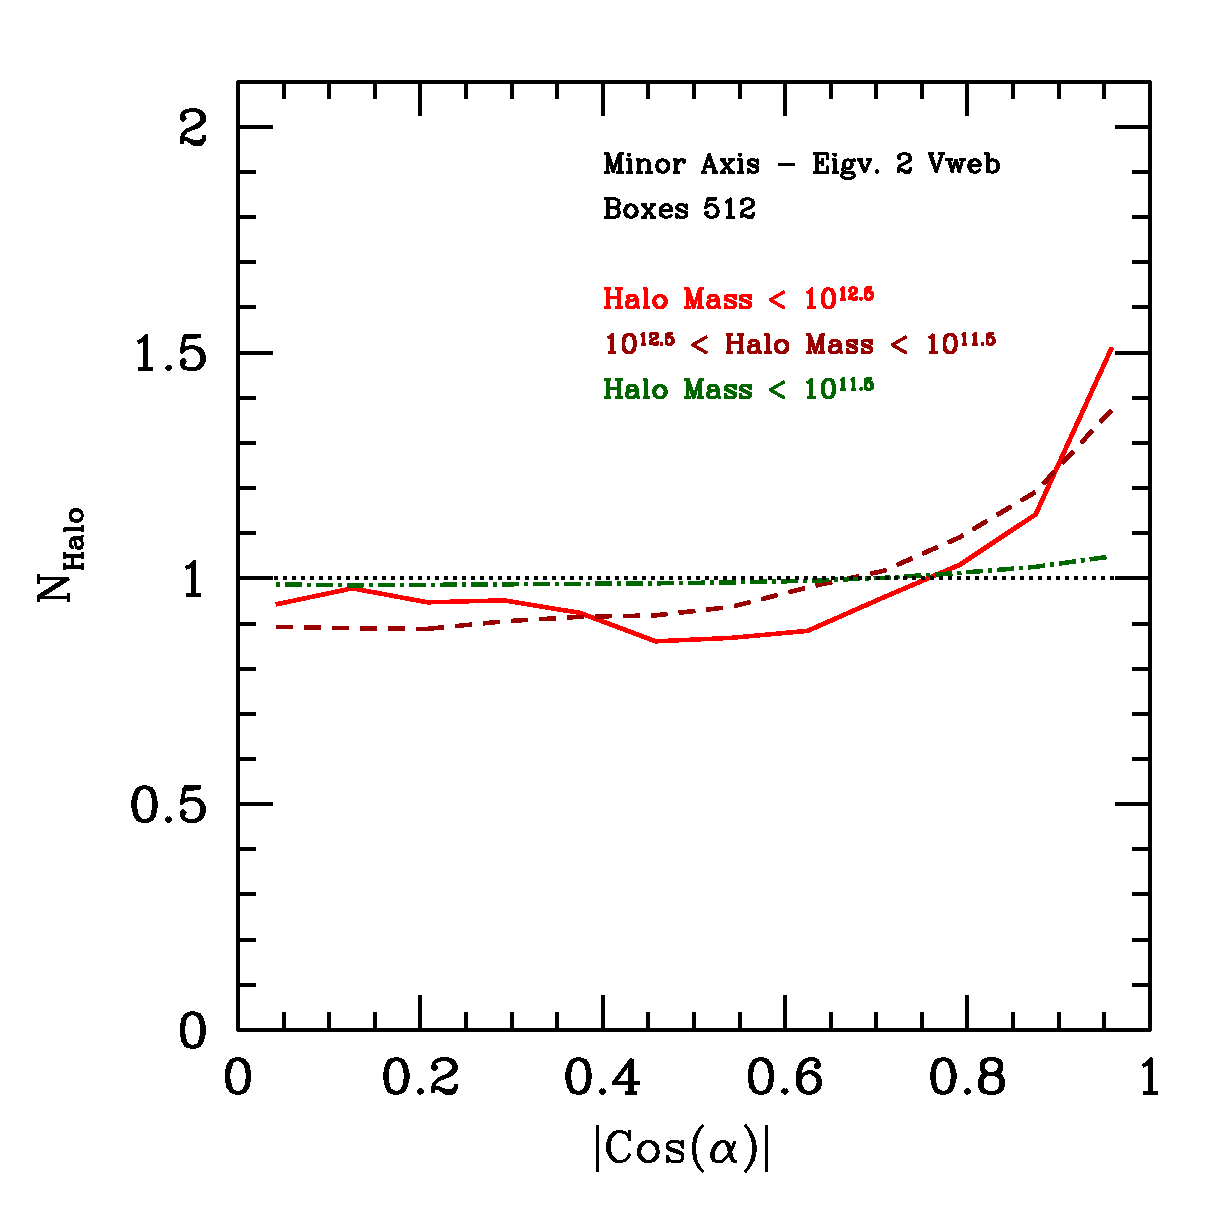
\includegraphics[width=0.30\textwidth]{../plot2/Ax3_VT/512_AX3_V2.ps}
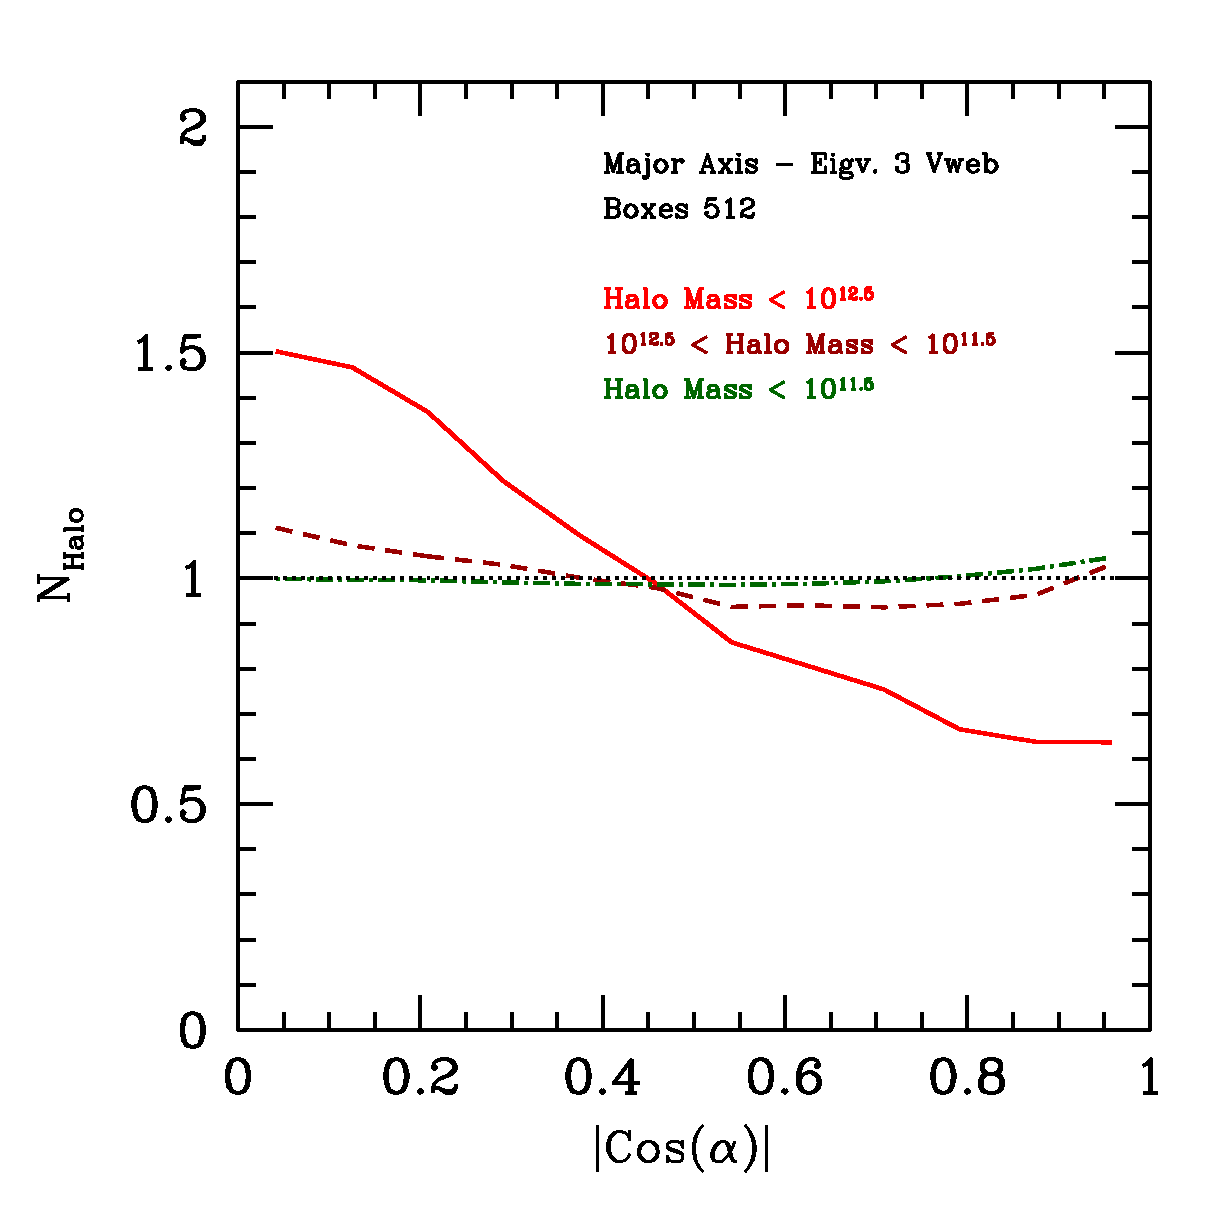
\includegraphics[width=0.30\textwidth]{../plot2/Ax1_VT/512_AX1_V3.ps}
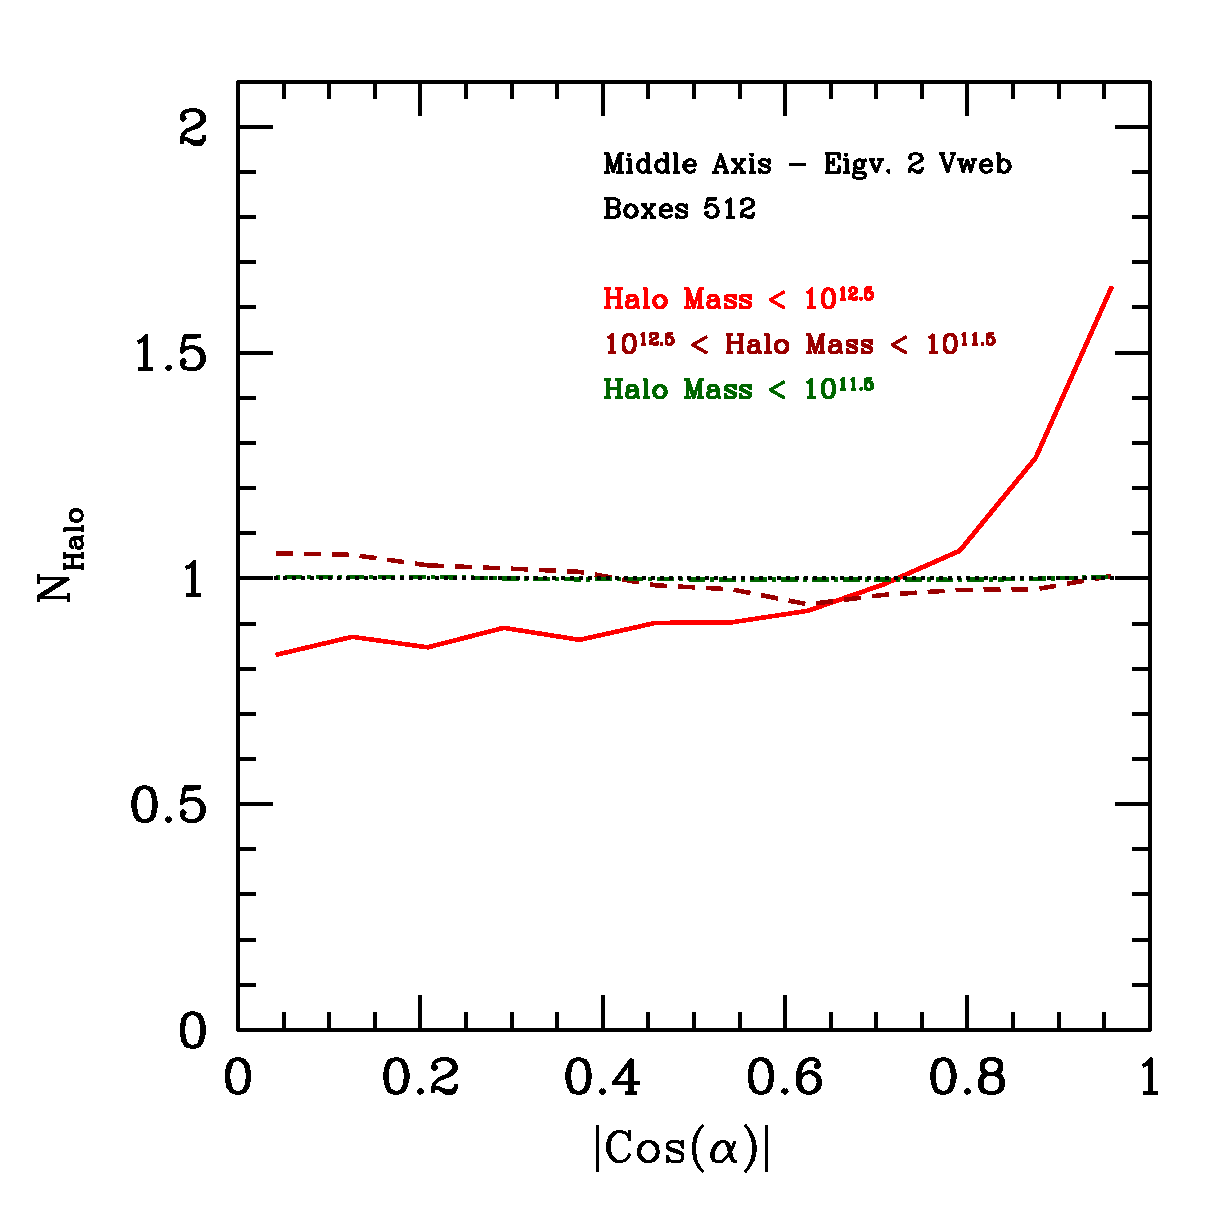
\includegraphics[width=0.30\textwidth]{../plot2/Ax2_VT/512_AX2_V2.ps}
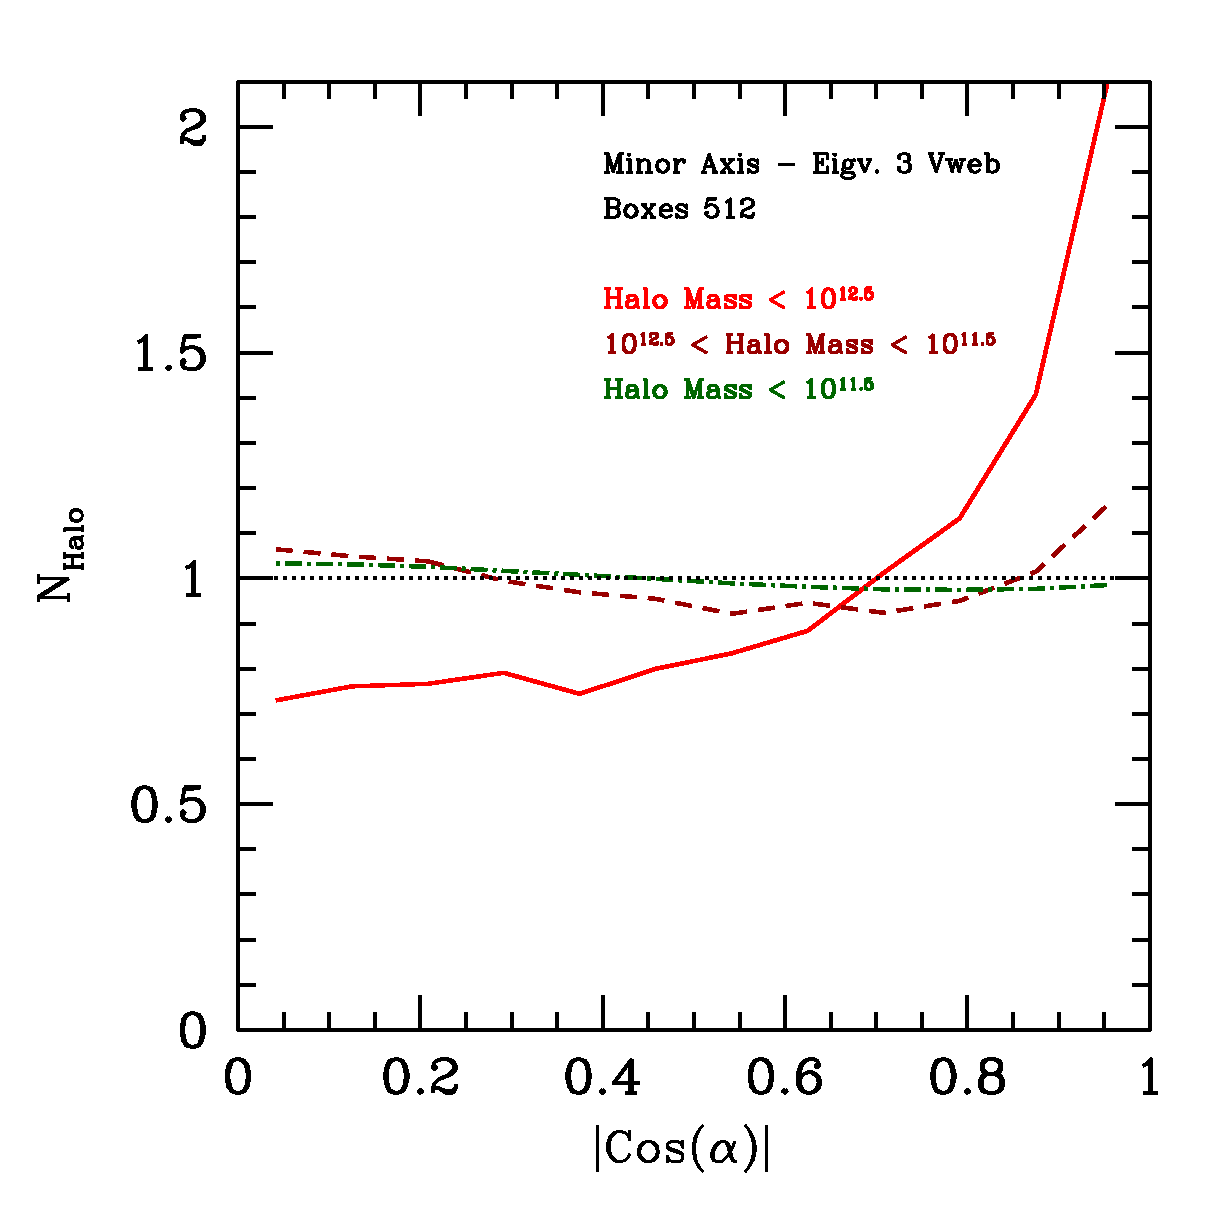
\includegraphics[width=0.30\textwidth]{../plot2/Ax3_VT/512_AX3_V3.ps}
\caption{Shape alignment for the vweb at $512^3$ resolution.}
\end{figure*}

\begin{figure*}
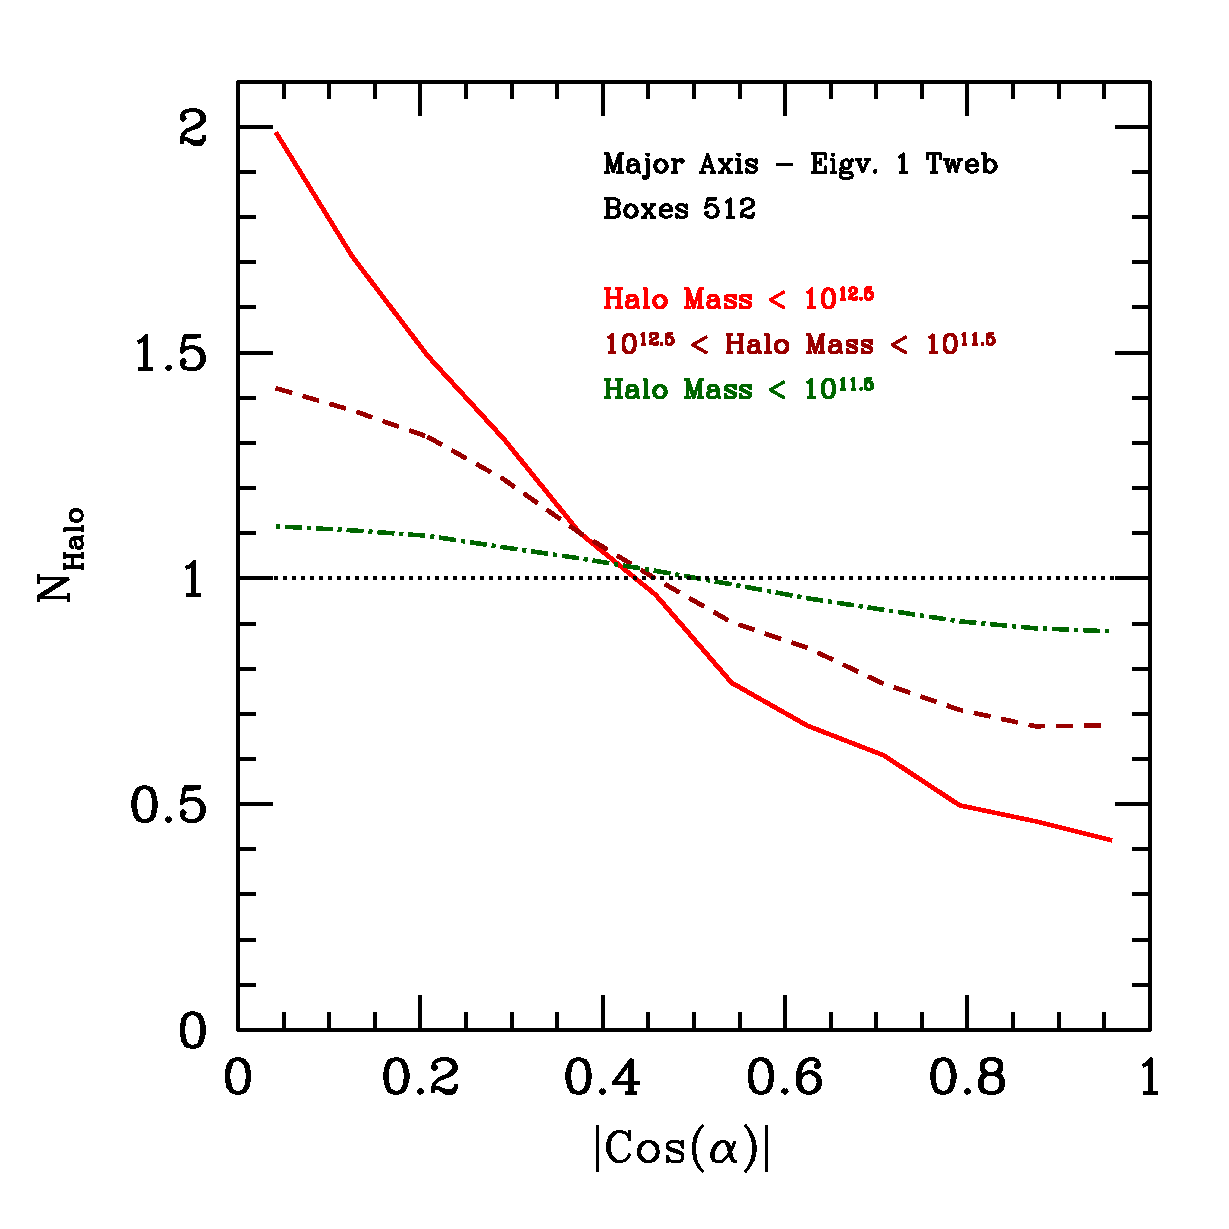
\includegraphics[width=0.30\textwidth]{../plot2/Ax1_VT/512_AX1_T1.ps}
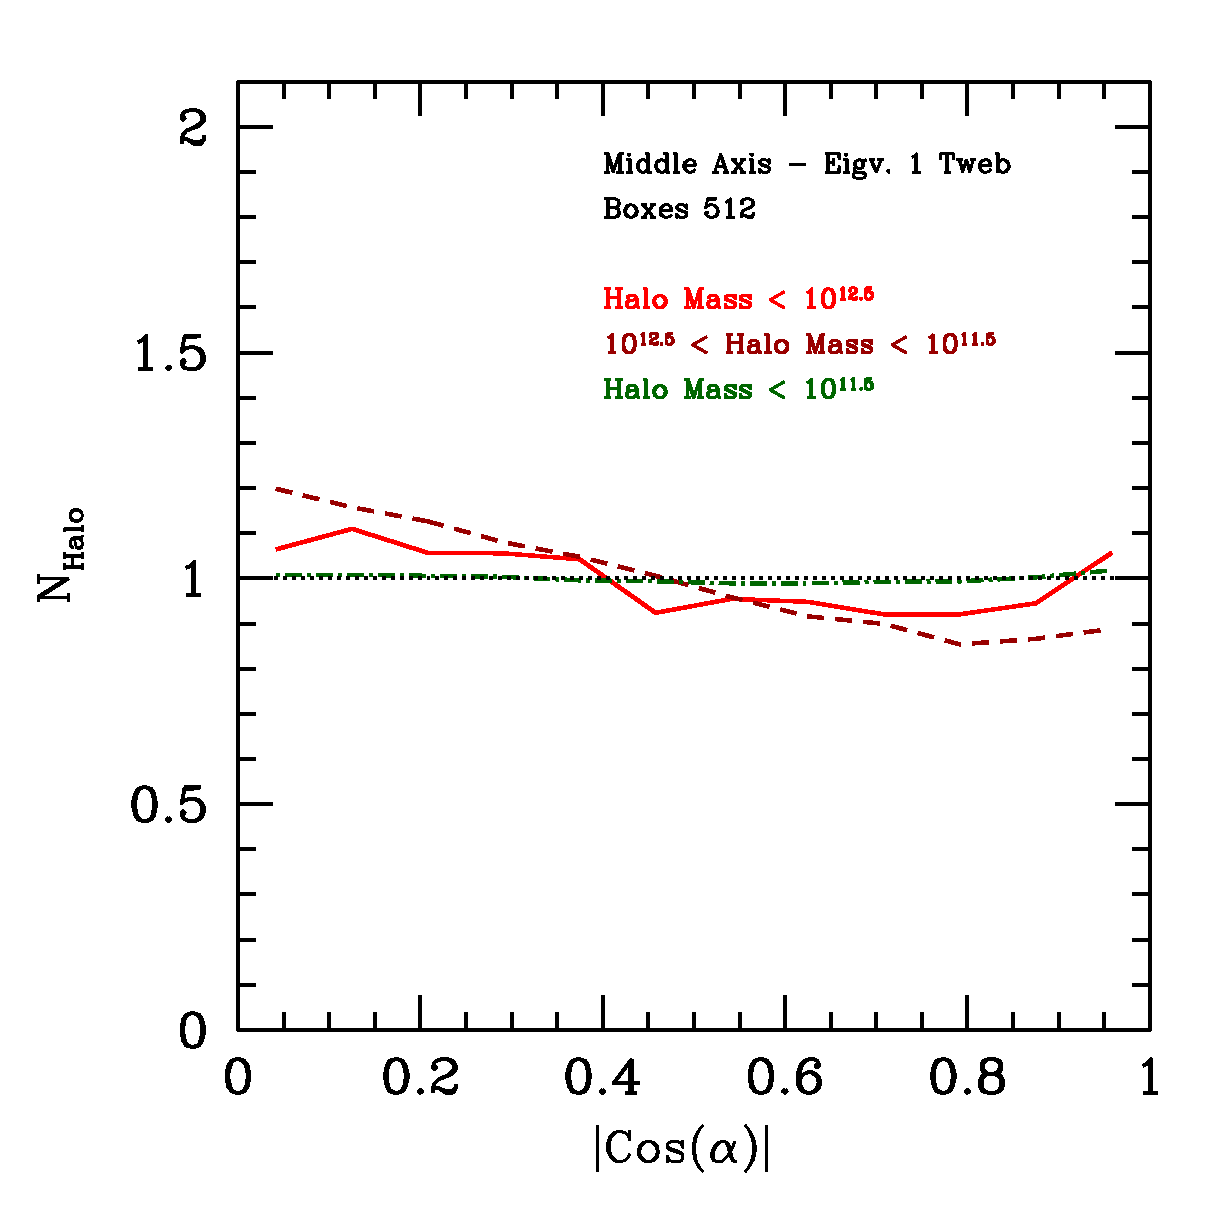
\includegraphics[width=0.30\textwidth]{../plot2/Ax2_VT/512_AX2_T1.ps}
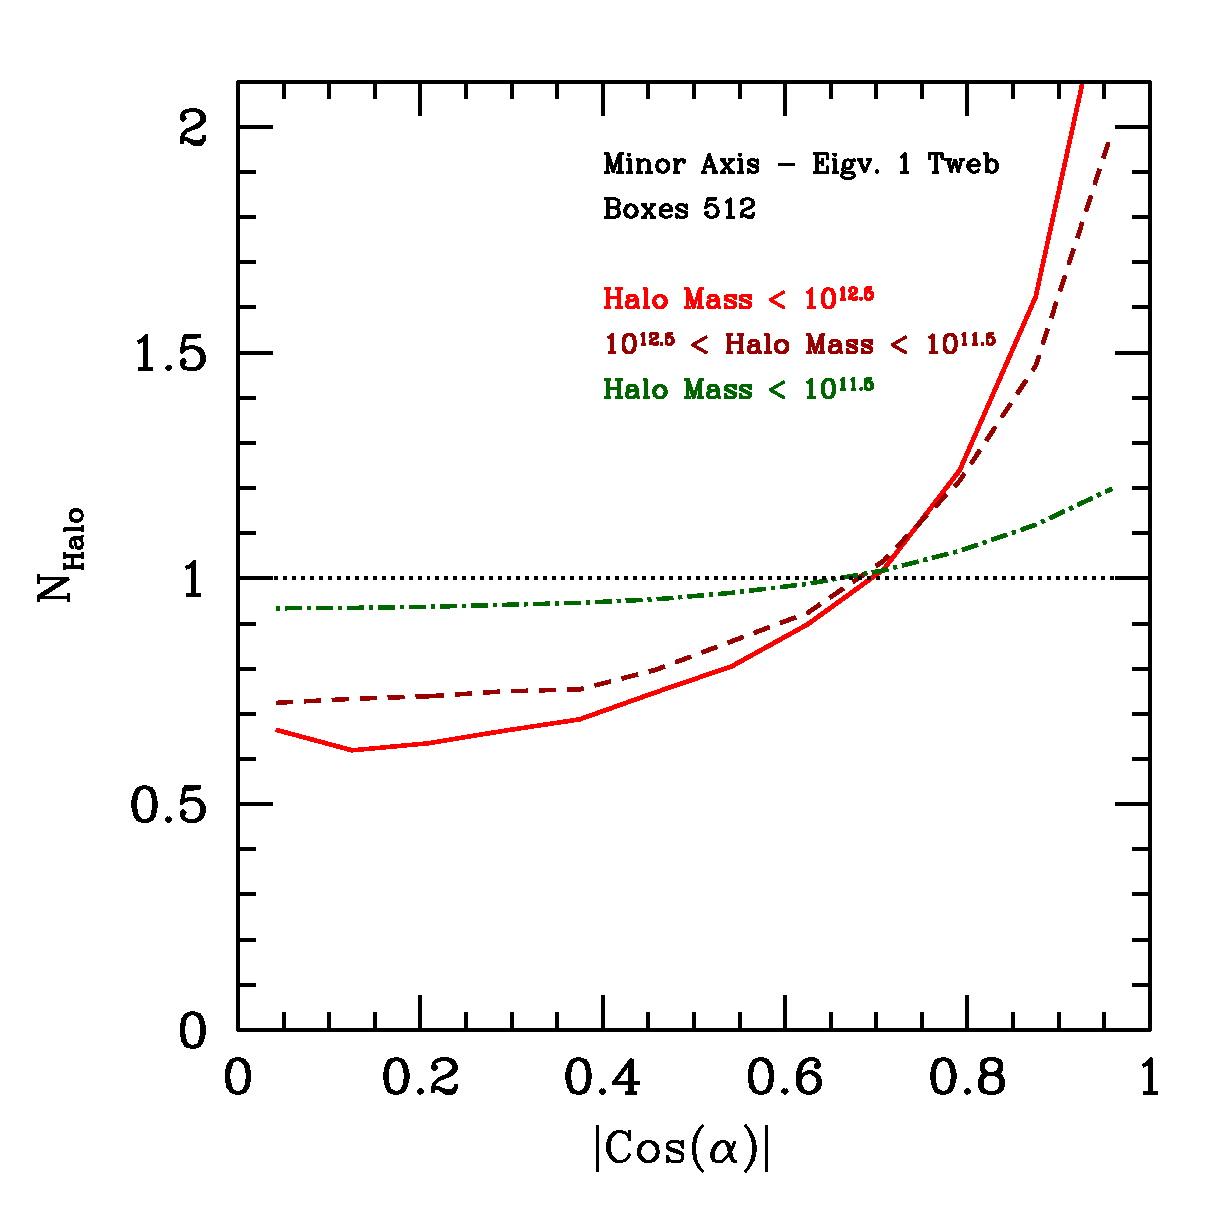
\includegraphics[width=0.30\textwidth]{../plot2/Ax3_VT/512_AX3_T1.ps}
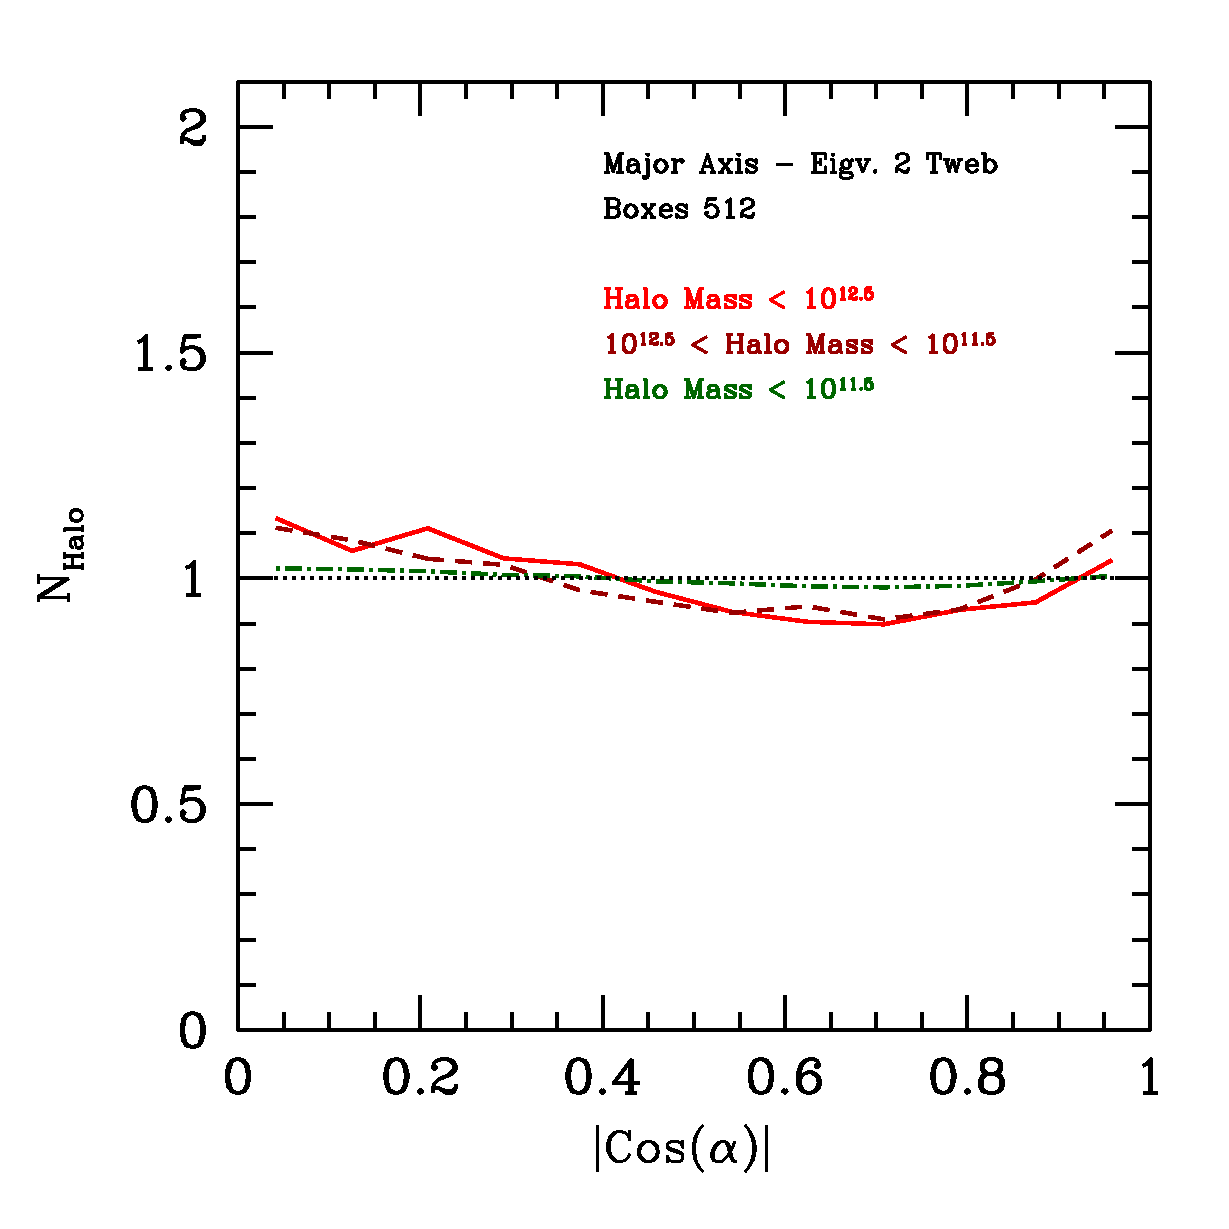
\includegraphics[width=0.30\textwidth]{../plot2/Ax1_VT/512_AX1_T2.ps}
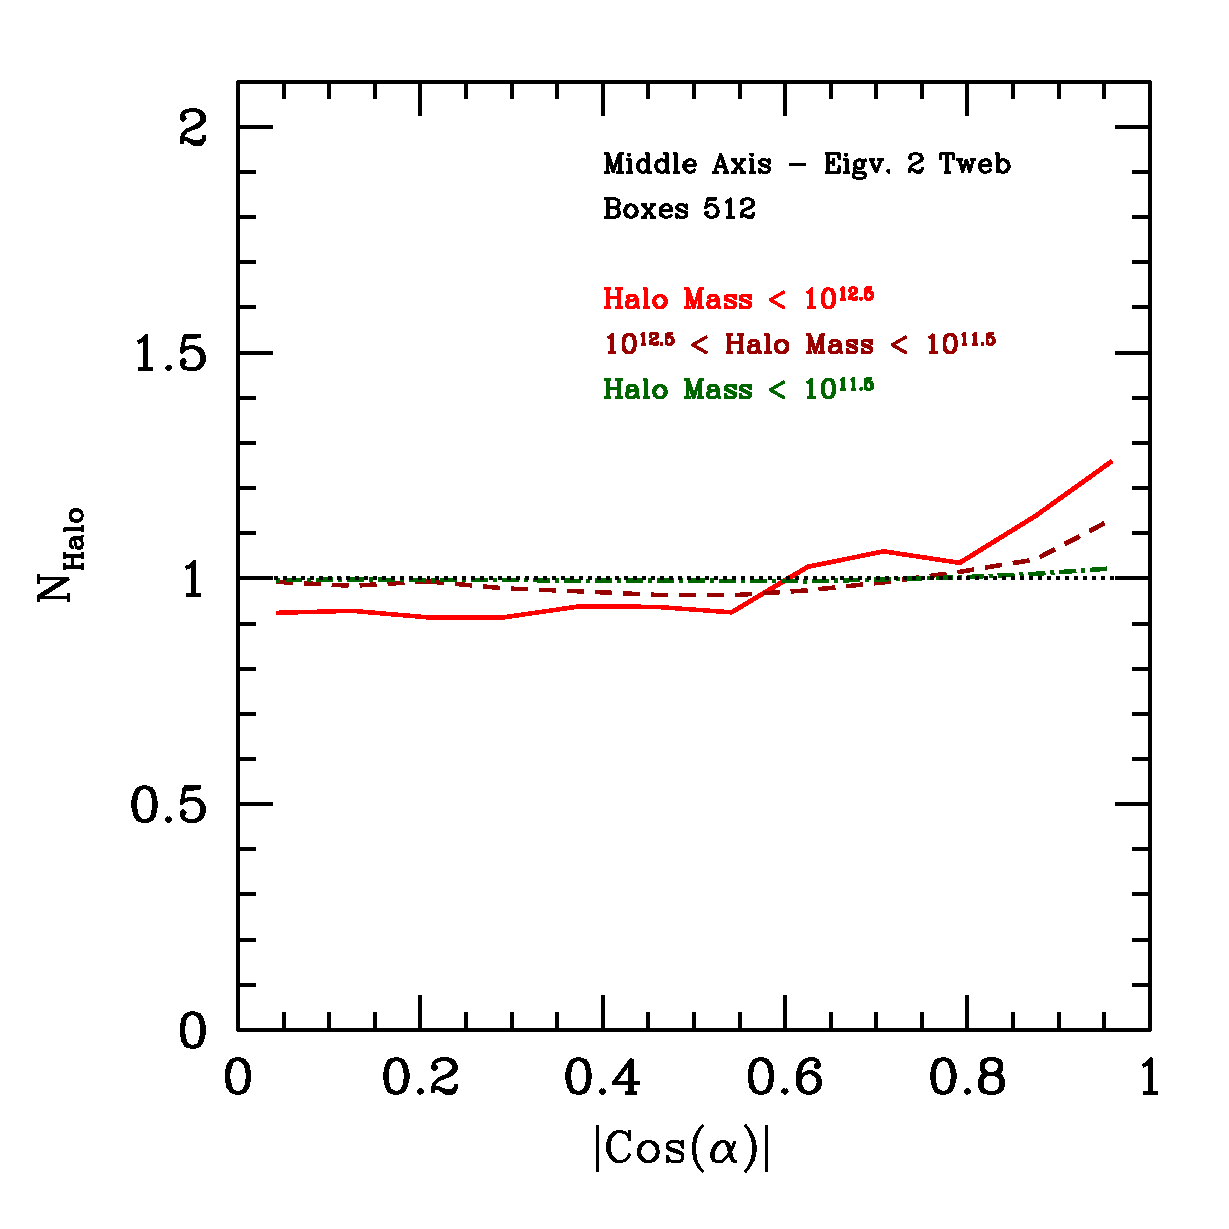
\includegraphics[width=0.30\textwidth]{../plot2/Ax2_VT/512_AX2_T2.ps}
\includegraphics[width=0.30\textwidth]{../plot2/Ax3_VT/512_AX3_T2.ps}
\includegraphics[width=0.30\textwidth]{../plot2/Ax1_VT/512_AX1_T3.ps}
\includegraphics[width=0.30\textwidth]{../plot2/Ax2_VT/512_AX2_T2.ps}
\includegraphics[width=0.30\textwidth]{../plot2/Ax3_VT/512_AX3_T3.ps}
\caption{Shape alignment for the tweb at $512^3$ resolution.}
\end{figure*}




\newpage
\subsection{Angular Momentum Alignment}

\begin{figure*}
\includegraphics[width=0.30\textwidth]{../plot2/J/256_J_V1.ps}
\includegraphics[width=0.30\textwidth]{../plot2/J/256_J_V2.ps}
\includegraphics[width=0.30\textwidth]{../plot2/J/256_J_V3.ps}
\caption{Angular momentum alignment with the Vweb for $256^3$ grid resolution.}
\end{figure*}


\begin{figure*}
\includegraphics[width=0.30\textwidth]{../plot2/J/512_J_V1.ps}
\includegraphics[width=0.30\textwidth]{../plot2/J/512_J_V2.ps}
\includegraphics[width=0.30\textwidth]{../plot2/J/512_J_V3.ps}
\caption{Angular momentum alignment with the Vweb for $512^3$ grid resolution.}
\end{figure*}


\begin{figure*}
\includegraphics[width=0.30\textwidth]{../plot2/J/256_J_T1.ps}
\includegraphics[width=0.30\textwidth]{../plot2/J/256_J_T2.ps}
\includegraphics[width=0.30\textwidth]{../plot2/J/256_J_T3.ps}
\caption{Angular momentum alignment with the Tweb for $256^3$ grid resolution.}
\end{figure*}


\begin{figure*}
\includegraphics[width=0.30\textwidth]{../plot2/J/512_J_T1.ps}
\includegraphics[width=0.30\textwidth]{../plot2/J/512_J_T2.ps}
\includegraphics[width=0.30\textwidth]{../plot2/J/512_J_T3.ps}
\caption{Angular momentum alignment with the Tweb for $512^3$ grid resolution.}
\end{figure*}



\subsection{Peculiar velocity Alignment}

\begin{figure*}
\includegraphics[width=0.30\textwidth]{../plot2/Vel/256_vel_V1.ps}
\includegraphics[width=0.30\textwidth]{../plot2/Vel/256_vel_V2.ps}
\includegraphics[width=0.30\textwidth]{../plot2/Vel/256_vel_V3.ps}
\caption{Peculiar velocity alignment with the Vweb for $256^3$ grid resolution.}
\end{figure*}


\begin{figure*}
\includegraphics[width=0.30\textwidth]{../plot2/Vel/512_vel_V1.ps}
\includegraphics[width=0.30\textwidth]{../plot2/Vel/512_vel_V2.ps}
\includegraphics[width=0.30\textwidth]{../plot2/Vel/512_vel_V3.ps}
\caption{Peculiar velocity alignment with the Vweb for $512^3$ grid resolution.}
\end{figure*}


\begin{figure*}
\includegraphics[width=0.30\textwidth]{../plot2/Vel/256_vel_T1.ps}
\includegraphics[width=0.30\textwidth]{../plot2/Vel/256_vel_T2.ps}
\includegraphics[width=0.30\textwidth]{../plot2/Vel/256_vel_T3.ps}
\caption{Peculiar velocity alignment with the Tweb for $256^3$ grid resolution.}
\end{figure*}


\begin{figure*}
\includegraphics[width=0.30\textwidth]{../plot2/Vel/512_vel_T1.ps}
\includegraphics[width=0.30\textwidth]{../plot2/Vel/512_vel_T2.ps}
\includegraphics[width=0.30\textwidth]{../plot2/Vel/512_vel_T3.ps}
\caption{Peculiar velocity alignment with the Tweb for $512^3$ grid resolution.}
\end{figure*}



\section{Discussion}
\label{sec:discussion}


\section{Conclusions}
\label{sec:conclusions}


\section*{Acknowledgments} 

\bibliographystyle{mn2e}
\bibliography{references} 



\end{document}
